%!TEX root = ../main.tex

%%%%%%%%%%%%%%%%%%%%%%%%%%%%%%%
%%%%%%%%%%%%%%%%%%%%%%%%%%%%%%%
\chapter{Fundamentals}
% Evtl. lieber Basics nennen; Stand der Technik ist es ja nicht wirklich
\label{chap:fundamentals}

\commenting{Input of basic knowledge for system modelling; Maybe supplementary knowledge} \mycomment[MK]{Write Chap Fundamentals}

General sources in terms of standard literature: \autocite{oedingElektrischeKraftwerkeUnd2016,gloverPowerSystemAnalysis2017,kundurPowerSystemStability2022,machowskiPowerSystemDynamics2020}

%%%%%%%%%%%%%%%%%%%%%%%%%%%%%%%
\section{Basics synchronous generators}
\label{sec:basics-sg}
\commenting{
        \begin{itemize}
                \item characteristics of a synchronous generator; structure and types of SG's
                \item mathematical background and description of the behavior -> dynamic modelling
                \item \textbf{Swing equations}
                \item Damping: not interesiting for us
        \end{itemize}
}

The final swing equation system can be derived to following two equations, which have to be solved in every time step to determine the pole angle $\delta$ and the rotor speed $\omega$, respectively the rotor speed change from its base value $\Delta\omega$:
\begin{align}
        \frac{d\delta}{dt}       & =\Delta\omega \label{eq:swing1}                                                         \\[12pt]
        \frac{d\Delta\omega}{dt} & =\frac{1}{2 \cdot H_\mathrm{gen}} \cdot (P_\mathrm{m} - P_\mathrm{e}) \label{eq:swing2}
\end{align}
% where

% \begin{tabularx}{\textwidth}[H]{ll}
%         $\delta$                & power angle \\
%         $\Delta\omega$          & change of rotor angular speed \\
%         $H_\mathrm{gen}$        & inertia constant of the \acs{SG} \\
%         $P_\mathrm{m}$          & mechanical power of the turbine \\
%         $P_\mathrm{e}$          & electrical power demanded transferred out of the \acs{SG}
% \end{tabularx}
% \vspace{12pt}

The generation of a \ac{TDS} for this equation system takes place in \autoref{sec:tds}.

%%%%%%%%%%%%%%%%%%%%%%%%%%%%%%%
\section{System stability esp. transient context}
\commenting{
        \begin{itemize}
                \item What is to be analyzed? And why? -> different stability analysis
                \item rotor angle stability,
                \item \textbf{derivation of EAC,}
                \item basic assessment models (single machine infinite bus, see \autocite{kundurPowerSystemStability2022})
        \end{itemize}
}

With respect to the limitations, that
\begin{enumerate}
        \item the machine is operating under balanced three-phase positive-sequence conditions,
        \item the machine excitation is constant,
        \item the machine losses, saturation, and saliency are neglected,
\end{enumerate}
a simplified \acf{SMIB} model can be considered for transient stability assessment (see \autoref{fig:smib-model}).  The \ac{IBB} is working with a constant voltage $E_\mathrm{ibb}$ and angle $\delta_\mathrm{ibb}$, typically set to $0^\circ$. The real power flowing from the \ac{SG} to the \ac{IBB} is then expressed within the \autoref{eq:p_e} and only dependent on the power angle $\delta$. The reactance $X_\mathrm{res}$ is expressing the simplified reactance from the respective circuit.
\begin{align}
        P_\mathrm{e}=\frac{E_\mathrm{p} \cdot E_\mathrm{ibb}}{X_\mathrm{res}} \cdot sin(\delta) \label{eq:p_e}
\end{align}
The mechanical power of the turbine is assumed constant, due to the short occurance of transient stability problems.

\begin{figure}[H]
        \centering
        \vspace{1cm}
        \begin{circuitikz}[european, scale=.9, smallR/.style={resistor,resistors/scale=.7}]
                \draw (0,0) node[oscillator, anchor=east, name=gen]{} --(.5,0)
                to[L, name=X_g] ++(2,0) coordinate(f1)
                \bushere{1}{$\underline{E}_\mathrm{T}'$}{}
                to[oosourcetrans,prim=delta,sec=wye] ++(2,0)
                \bushere{1.25}{$\underline{E}_\mathrm{T}''$}{} coordinate(b1) ++(0,-.5) -- coordinate(f2) ++(1.5,0)
                to[L, name=X_l2] ++(1,0) -- ++(1.5,0) ++(0,.5)
                \bushere{1.25}{$\underline{E}_\mathrm{ibb}$}{} ++(0,.5) coordinate(b2) ++(0,-.5) -- coordinate(f3) ++(1,0)
                node[gridnode, anchor=left, name=ib]{};
                \draw (b1) ++(0,.5) to[L, name=X_l1] (b2);
                % \draw[line width=2pt] (2.25,1) -- (2.25,-1);
                % \draw[line width=2pt] (4.75,1) -- (4.75,-1);
                % \draw[line width=2pt] (8.25,1) -- (8.25,-1);
                \node[above=6pt] at (X_g) {$X_\mathrm{g}'$};
                \node[above=6pt] at (X_l1) {$X_\mathrm{l}$};
                \node[below=6pt] at (X_l2) {$X_\mathrm{l}$};
                \path[->] (-1.2,.5) edge [bend right] node[left=6pt]{$E_\mathrm{p}~\angle~\delta$} (-1.2,-.5);
                \path[->] (ib) ++(.8,.5) edge [bend left] node[right=6pt]{$E_\mathrm{ibb}~\angle~0^{\circ}$} ++(0,-1);
                \draw[-Stealth, very thick, red] (f1) ++(0,-.5) -- ++(-.15,-.45) -- ++(.3,.2) -- ++(-.2,-.6) coordinate(f1_text);
                \node[below, red] at (f1_text) {\scriptsize fault 1};
                \draw[-Stealth, very thick, red] (f2) ++(0,.3) -- ++(-.15,-.45) -- ++(.3,.2) -- ++(-.2,-.6) coordinate(f2_text);
                \node[below, red] at (f2_text) {\scriptsize fault 2};
                \draw[-Stealth, very thick, red] (f3) ++(0,.3) -- ++(-.15,-.45) -- ++(.3,.2) -- ++(-.2,-.6) coordinate(f3_text);
                \node[below, red] at (f3_text) {\scriptsize fault 3};
        \end{circuitikz}
        \vspace{.5cm}
        \caption[Representative circuit of a \acf{SMIB} model]{Representative circuit of a \acf{SMIB} model with pole wheel voltage $E_\mathrm{p}~\angle~\delta$ and \acf{IBB} voltage $E_\mathrm{ibb}~\angle~0^{\circ}$; positions of considered faults 1 to 3 are marked with red lightning arrows}
        \label{fig:smib-model}
\end{figure}
% where

% \begin{tabularx}{\textwidth}[H]{lX}
%         $\delta$                        & power angle \\
%         $E_\mathrm{p}$                  & pole potential of the \acf{SG} \\
%         $\underline{E}_\mathrm{T}'$     & complex potential on the primary side of the transformer \\
%         $\underline{E}_\mathrm{T}''$    & complex potential on the secondary side of the transformer \\
%         $\underline{E}_\mathrm{ibb}$    & complex pole potential of the \acf{IBB} \\
%         $X_\mathrm{g}'$                 & reactance of the \acf{SG} \\
%         $X_\mathrm{l}$                  & reactance of a single line \\
% \end{tabularx}

%%%%%%%%%%%%%%%%%%%%%%%%%%%%%%%
% \section{Events harming the system stability}
% \commenting{
%         \begin{itemize}
%                 \item \textbf{fault types,}
%                 \item load-changes
%                 \item effects of electrical networks (esp. generator networks) vs. single machine systems -> paper \autocite{batchuComparativeStudyEqual2022}: IBB not that extremely fixed, group of critical and non-critical machines; but more of an outlook and targeting real-time calculation (for system operation)
%         \end{itemize}
% }

% The electrical energy system or network is a balance of power input (generation) and output (use). Changes and dynamics of this balance lead to system answers, which can result in a remaining stable system, or unlikely an unstable system. When specifically the generator is moving into an unstable operation, and can not stay in synchronous and stable speed with the rest of the system, it has to be disconnected from the power grid.

% \begin{figure}[h]
%         \centering
%         \vspace{12pt}
%         \begin{tikzpicture}[sibling distance=30mm, every node/.style={rectangle, draw, align = center, rounded corners=5pt, minimum height=24pt, font=\footnotesize}], %line width = 1, minimum width = 30mm, minimum height = 7mm,}]
%                 \node {Stability harming events}
%                 child {node {short circuit}
%                         child {node {three-phase}
%                                 child {node {complete}}
%                                 child {node {partial}}}
%                         child {node {single-phase}}}
%                 child {node {load change}};
%         \end{tikzpicture}
%         \caption{Overview of events harming the system stability of a power grid}
%         \label{fig:stability-events}
% \end{figure}

% Events that can harm the system stability are sketched in \autoref{fig:stability-events}. This \arbeit~is interested in a three-phase short circuit, in the variants near a generator, far away of a generator and with a partial loss of a connecting overhead line.
\newpage
\section{Analytical calculation of the critical clearing time}
\label{sec:analytical-method}

\mycomment[MK]{make text in image bigger}
\begin{wrapfigure}{r}{.6\textwidth}
        \centering
        % \missingfigure[figwidth=.4\textwidth]{Equal are criterion visualization}
        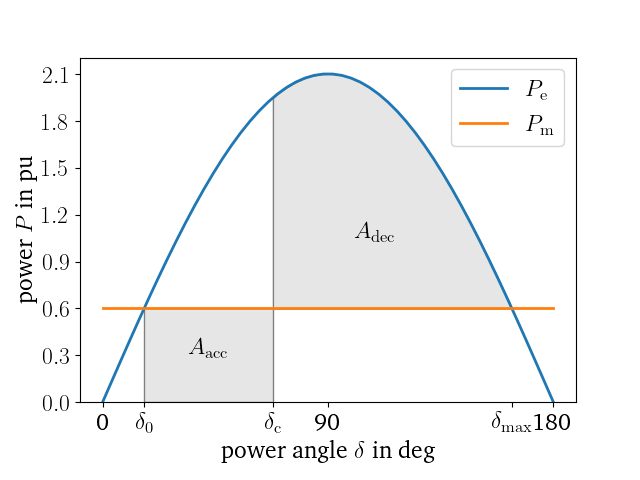
\includegraphics[width=.6\textwidth]{python/plots/eac.png}
        \caption{Illustrated \acf{EAC} in the P-$\delta$-curve}
        \label{fig:eac}
\end{wrapfigure}
For the analytical solution of the swing equation and following the \acs{CCT}, there is the need to find the critical power angle $\delta_\mathrm{cc}$ first. For this, the most common approach is the \acf{EAC}, considering that the amount of stored energy through acceleration (during the short or failure) is equal to the released energy (decelerating the rotor) when synchronizing again. These both energys can be calculated through the area under the curve of the power difference $\Delta P=P_\mathrm{m}-P_\mathrm{e}$, while the accelerating area is between the first stable operating angle $\delta_\mathrm{0}$ and the clearing angle $\delta_\mathrm{c}$, the decelerating area between $\delta_\mathrm{c}$ and the maximum dynamically stable angle $\delta_\mathrm{max}$. \autoref{fig:eac} is illustrating this approach. Following this approach a generalized expression is formed to
\begin{align}
        \int_{\delta_\mathrm{0}}^{\delta_\mathrm{1}}\Delta P~d\delta = 0 \label{eq:gen-eac},
\end{align}
while the more expressive can be achieved through splitting up the integral borders and equalize both areas:
\begin{align}
        % A_\mathrm{acc}=A_\mathrm{dec} \nonumber \\
        \int_{\delta_\mathrm{0}}^{\delta_\mathrm{c}}(P_\mathrm{m}-P_\mathrm{e})~d\delta = \int_{\delta_\mathrm{c}}^{\delta_\mathrm{max}}(P_\mathrm{e}-P_\mathrm{m})~d\delta \label{eq:big-eac}
\end{align}
With consideration of $\delta_\mathrm{max}=\pi-\delta_\mathrm{0}$ and $P_\mathrm{m}=P_\mathrm{max} \cdot sin(\delta_\mathrm{0})$, and some rearrangements, this leads to the final expression of the critical clearing angle:
\begin{align}
        \delta_\mathrm{cc}=arccos\big[~sin(\delta_\mathrm{0}) \cdot (\pi-2 \cdot \delta_\mathrm{0})-cos(\delta_\mathrm{0})~\big] \label{eq:delta-cc}
\end{align}

The second step is the calculation of the \acs{CCT} dependent on the critical clearing angle. Splitting the differentiated variables $d^2\delta$ and $dt$ in the combined swing equation and integrating twice, leads to the equation
\begin{align}
        \delta=\frac{\omega \cdot \Delta P}{4 H_\mathrm{gen}} \cdot t^2 + \delta_\mathrm{0}. \nonumber
\end{align}
Rearranging this gives an expression for calculating the critical clearing time $t_\mathrm{cc}$ (see \autoref{eq:tcc}).
\begin{align}
        t_\mathrm{cc}=\sqrt{\frac{4 H_\mathrm{gen} \cdot (\delta_\mathrm{c}-\delta_\mathrm{0})}{\omega \cdot \Delta P}} \label{eq:tcc}
\end{align}

%%%%%%%%%%%%%%%%%%%%%%%%%%%%%%%
\section{Numerical methods for system modeling}
\commenting{
        \begin{itemize}
                \item \textbf{solving second order ODEs (explicit)}
                \item Differentiation explicit/impolicit, inertial value problems, boundary value problems, ...
        \end{itemize}
}

System dynamics is a method for describing, understand, and discuss complex problems in the context of system theory \textbf{[SOURCE]}. They often can be described through a set of coupled \acfp{ODE}, most resoluted in time dimension. \commenting{How to bridge towards different boundary types, explicit and implicit methods, ...; Different solving methods, ..., Dirichlet-boundaries, von-Neumann-boundaries, ...}

\acsp{ODE} can be solved through numerical integration with different methods. An easy and less complex method is Euler's method. It uses a linear extrapolation to calculate the functions value at the next timestep, so following the iterable function
\begin{align}
        f_\mathrm{t+1}=f_\mathrm{t}+\left(\frac{df}{dt}\right)_\mathrm{t} \cdot \Delta t \label{eq:euler},
\end{align}
with $t$ being the time and $f$ an on $t$ dependent function. Generally a system of second order \acsp{ODE} can be rewritten as two first order equations. This often simplifies the calculation or the use of numerical methods. The presented swing equation of a \acs{SG} in \autoref{eq:swing1} and \autoref{eq:swing2} has been split up by that principle.

%%%%%%%%%%%%%%%%%%%%%%%%%%%%%%%
%%%%%%%%%%%%%%%%%%%%%%%%%%%%%%%
\chapter{Numerical modelling}
\label{chap:methods}

Following chapter will describe the implementation of Python Code for solving the derived \acs{ODE} system (see \autoref{sec:basics-sg}). For this the Python version 3.9 was used, in combination with the packages scipy, numpy, and matplotlib.\footnote{documentation and manual can be found on \href{https://scipy.org/}{\itshape https://scipy.org/} \autocite{virtanenSciPyFundamentalAlgorithms2020}, similiar for \href{https://matplotlib.org/}{\itshape matplotlib}, and \href{https://numpy.org/}{\itshape numpy} packages} The complete code is included in the \autoref{app:code}. \mycomment[MK]{Write Chap Methods}

%%%%%%%%%%%%%%%%%%%%%%%%%%%%%%%
\section{Structure of the \acs{CCT} assessment}
\commenting{
        Program plan for determination / algorithm structure, containing:
        \begin{itemize}
                \item Pre questions:
                      \begin{enumerate}
                              \item What do I want to know from the algorithm?
                              \item What do I want to see?
                      \end{enumerate}
                \item Answers / Hints for the algorithm:
                      \begin{enumerate}
                              \item What are needed inputs?
                              \item What are needed functions?
                              \item How do partial results interact with each other / puzzle together to the superior question?
                      \end{enumerate}
        \end{itemize}
}

\begin{figure}[H]
        \centering
        \begin{tikzpicture}[node distance = 1.5cm, auto]
                % Place nodes
                \node [papStart] (Start1){Start};
                \node [papProcess, below of = Start1,label={[shift={(2.7,-0.6)}]\footnotesize\textit{label 1}}] (pro1){Prozess};
                \node [papProcess, below of = pro1,label={[shift={(3,-0.6)}]\footnotesize\textit{label 2}}](pro2){Prozess};
                \node [papDecision, below of = pro2, yshift= -9mm](dec1){Entscheidung};
                \node [papPredProc,  right of = dec1, xshift=25mm](predproc1){\nodepart{two}\shortstack{vordefinierter\\Prozess}};
                \node [papProcess, below of = predproc1,label={[shift={(2.3,-0.6)}]\footnotesize\textit{label 3}}](pro3){Prozess};
                \node [papEnd, below of = dec1, yshift= -20mm] (End) {Ende};

                % Place joins
                \coordinate [below of = dec1, yshift= -10mm] (join1);

                % Draw edges
                \path [papLine] (Start1) -- (pro1);
                \path [papLine] (pro1) -- (pro2);
                \path [papLine] (pro2) -- (dec1);
                \path [papLine] (dec1) -- node [right] {\papYes} (End);
                \path [papLine] (dec1) -- node [above] {\papNo} (predproc1);
                \path [papLine] (predproc1) -- (pro3);
                \path [papLine] (pro3) |- (join1);
        \end{tikzpicture}
        \caption{Program plan for determining the \acf{CCT}}
        \label{fig:program-plan}
\end{figure}

%%%%%%%%%%%%%%%%%%%%%%%%%%%%%%%
\section{Electrical simplifications and scenario setting}
\label{sec:scenario}
\commenting{
        \begin{itemize}
                \item Simplification of all the components in SMIB network to a simple network
                \item Transforming into symmetrical components (for determination of shorts -> e.g. transformer)
        \end{itemize}
}

\subsection{Electric networks}
\missingfigure{Simplified networks, which are in interest and shall be simulated with the algorithm; ideally solved with subfigures}

\subsection{Simulation cases and boundaries}
\label{sec:sim-boundaries}

The boundaries of the single cases, which are simulated, are given with a Python dictionary. Therefore the values of the variables have to be predefined and documented. Considering fault cases, there are three differences in the interest:
\begin{enumerate}
        \item A full line fault, meaning the complete electrical power is disconnected. The \acs{CCT} of the fault has to be determined, a \acs{TDS} with fault clearing shortly before and after the critical clearing is carried out and displayed as {\itshape stable} and {\itshape unstable};
        \item A partial line fault, meaning just a defined percentage of the electrical power is disconnected. The further evaluation is carried out like in scenario 1.;
        \item A partial line fault, meaning just a defined percentage of the electrical power is disconnected. But with consideration, that the fault condition is stable at a new operation point. This point is calculated in the time domain.
\end{enumerate}
Further of interest is a parameter variation of both influences $H_\mathrm{gen}$ and $\Delta P$. This last parameter is not meant to describe the absolute power difference, which is inserted into the swing equation, but more the power difference relative to the maximum electrical power output of the generator. Due to the relation between the maximum power output and the disconnected electrical power in the acceleration and deceleration of the rotor, it seems more significant to use this as a relative parameter. The \acs{CCT} in dependency of these two influences shall be elaborated.

Lastly, a comparison between calculating with the algebraic equation system of the network and the calculation solely with the power flowing dependent on both (fixed) bus voltages, the reactance and the power angle takes place.

\subsection{Initial value calculation}
\commenting{
        \begin{itemize}
                \item Load flow analysis
                \item Calculation of $E_\mathrm{i}$, $I_\mathrm{i}$, $P_\mathrm{i}$, $\delta_\mathrm{i}$, ..., as well for IBB
        \end{itemize}
}

%%%%%%%%%%%%%%%%%%%%%%%%%%%%%%%
\section{Implementation of the time domain solution}
\label{sec:tds}

\commenting{
        \begin{itemize}
                \item Different levels of TDS; With/without solving of algebraic equations at each timestep; With/without calculation of turbine momentum at each timestep (dependent on omega)
                \item Utilization as a function: calculation with clearing and without clearing: for determination of CCT needed
        \end{itemize}
}

%%%%%%%%%%%%%%%%%%%%%%%%%%%%%%%
\section{Implementation of the equal area criterion}

\commenting{
        \begin{itemize}
                \item Iterative process needed? Due to omega and delta dependencies of $P_e$ and $P_m$
                \item Different methods of CCT calculation: P-$\delta$-curve; P-t-curves
        \end{itemize}
}


%%%%%%%%%%%%%%%%%%%%%%%%%%%%%%%
%%%%%%%%%%%%%%%%%%%%%%%%%%%%%%%
\chapter{Results}
\label{chap:results}

\mycomment[MK]{Write Chap Results}

%%%%%%%%%%%%%%%%%%%%%%%%%%%%%%%
\section{Analytical results}
\label{sec:analytical-results}

The analytical calculation follows the equations from \autoref{sec:analytical-method}. Therefore the base values for the three input scenarios are used. The results of this calculation are shown in \autoref{tab:res-analytical}.

\begin{table}[H]
        \small
        \centering
        \caption[Analytical results for the three fault-scenarios]{Analytical results for the three fault-scenarios; considering $\delta_\mathrm{cc}$ and $t_\mathrm{cc}$}
        \label{tab:res-analytical}
        \vspace{12pt}
        \begin{tabular}{|l|r|r|}
                \hline
                \rowcolor{lightgray} & $\delta_\mathrm{cc}$ in $\mathrm{deg}$ & $t_\mathrm{cc}$ in $\mathrm{s}$ \\ \hline \hline
                Fault 1              &                                        &                                 \\ \hline
        \end{tabular}
\end{table}

%%%%%%%%%%%%%%%%%%%%%%%%%%%%%%%
\section{Numerical results}

\autoref{tab:numerical-solutions} is summarizing the results for the \acs{CCT}-calculation of the different set scenarios in \autoref{sec:scenario}. The single scenarios are further described in the following.

\begin{table}[!htb]
        \small
        \centering
        \caption[Numerical results for \acs{CCT}-calculations]{Results ($CCT$ and $\delta_\mathrm{cc}$) for numerical solving the faults 1, 2, and 3}
        \label{tab:numerical-solutions}
        \vspace{12pt}
        \begin{tabular}{|l|r|r|}
                \hline
                \rowcolor{lightgray} Scenario & \acs{CCT} & $\delta_\mathrm{cc}$ \\ \hline \hline
                Fault 1                       &           &                      \\ \hline
                Fault 2                       &           &                      \\ \hline
                Fault 3                       &           &                      \\ \hline
        \end{tabular}
\end{table}

\subsection{Simulated faults}

\begin{figure}[H]
        \centering
        % \begin{subfigure}[b]{0.4\textwidth}
        % \centering
        %% Creator: Matplotlib, PGF backend
%%
%% To include the figure in your LaTeX document, write
%%   \input{<filename>.pgf}
%%
%% Make sure the required packages are loaded in your preamble
%%   \usepackage{pgf}
%%
%% Also ensure that all the required font packages are loaded; for instance,
%% the lmodern package is sometimes necessary when using math font.
%%   \usepackage{lmodern}
%%
%% Figures using additional raster images can only be included by \input if
%% they are in the same directory as the main LaTeX file. For loading figures
%% from other directories you can use the `import` package
%%   \usepackage{import}
%%
%% and then include the figures with
%%   \import{<path to file>}{<filename>.pgf}
%%
%% Matplotlib used the following preamble
%%   
%%   \usepackage{fontspec}
%%   \setmainfont{Charter.ttc}[Path=\detokenize{/System/Library/Fonts/Supplemental/}]
%%   \setsansfont{DejaVuSans.ttf}[Path=\detokenize{/opt/homebrew/lib/python3.10/site-packages/matplotlib/mpl-data/fonts/ttf/}]
%%   \setmonofont{DejaVuSansMono.ttf}[Path=\detokenize{/opt/homebrew/lib/python3.10/site-packages/matplotlib/mpl-data/fonts/ttf/}]
%%   \makeatletter\@ifpackageloaded{underscore}{}{\usepackage[strings]{underscore}}\makeatother
%%
\begingroup%
\makeatletter%
\begin{pgfpicture}%
\pgfpathrectangle{\pgfpointorigin}{\pgfqpoint{6.000000in}{8.000000in}}%
\pgfusepath{use as bounding box, clip}%
\begin{pgfscope}%
\pgfsetbuttcap%
\pgfsetmiterjoin%
\definecolor{currentfill}{rgb}{1.000000,1.000000,1.000000}%
\pgfsetfillcolor{currentfill}%
\pgfsetlinewidth{0.000000pt}%
\definecolor{currentstroke}{rgb}{1.000000,1.000000,1.000000}%
\pgfsetstrokecolor{currentstroke}%
\pgfsetdash{}{0pt}%
\pgfpathmoveto{\pgfqpoint{0.000000in}{0.000000in}}%
\pgfpathlineto{\pgfqpoint{6.000000in}{0.000000in}}%
\pgfpathlineto{\pgfqpoint{6.000000in}{8.000000in}}%
\pgfpathlineto{\pgfqpoint{0.000000in}{8.000000in}}%
\pgfpathlineto{\pgfqpoint{0.000000in}{0.000000in}}%
\pgfpathclose%
\pgfusepath{fill}%
\end{pgfscope}%
\begin{pgfscope}%
\pgfsetbuttcap%
\pgfsetmiterjoin%
\definecolor{currentfill}{rgb}{1.000000,1.000000,1.000000}%
\pgfsetfillcolor{currentfill}%
\pgfsetlinewidth{0.000000pt}%
\definecolor{currentstroke}{rgb}{0.000000,0.000000,0.000000}%
\pgfsetstrokecolor{currentstroke}%
\pgfsetstrokeopacity{0.000000}%
\pgfsetdash{}{0pt}%
\pgfpathmoveto{\pgfqpoint{0.750000in}{3.960000in}}%
\pgfpathlineto{\pgfqpoint{5.400000in}{3.960000in}}%
\pgfpathlineto{\pgfqpoint{5.400000in}{7.040000in}}%
\pgfpathlineto{\pgfqpoint{0.750000in}{7.040000in}}%
\pgfpathlineto{\pgfqpoint{0.750000in}{3.960000in}}%
\pgfpathclose%
\pgfusepath{fill}%
\end{pgfscope}%
\begin{pgfscope}%
\pgfpathrectangle{\pgfqpoint{0.750000in}{3.960000in}}{\pgfqpoint{4.650000in}{3.080000in}}%
\pgfusepath{clip}%
\pgfsetbuttcap%
\pgfsetroundjoin%
\definecolor{currentfill}{rgb}{0.900000,0.900000,0.900000}%
\pgfsetfillcolor{currentfill}%
\pgfsetlinewidth{1.003750pt}%
\definecolor{currentstroke}{rgb}{0.500000,0.500000,0.500000}%
\pgfsetstrokecolor{currentstroke}%
\pgfsetdash{}{0pt}%
\pgfsys@defobject{currentmarker}{\pgfqpoint{2.005500in}{3.960087in}}{\pgfqpoint{2.452054in}{6.161131in}}{%
\pgfpathmoveto{\pgfqpoint{2.005500in}{6.161131in}}%
\pgfpathlineto{\pgfqpoint{2.005500in}{3.960092in}}%
\pgfpathlineto{\pgfqpoint{2.014613in}{3.960092in}}%
\pgfpathlineto{\pgfqpoint{2.023727in}{3.960092in}}%
\pgfpathlineto{\pgfqpoint{2.032840in}{3.960091in}}%
\pgfpathlineto{\pgfqpoint{2.041953in}{3.960091in}}%
\pgfpathlineto{\pgfqpoint{2.051067in}{3.960091in}}%
\pgfpathlineto{\pgfqpoint{2.060180in}{3.960091in}}%
\pgfpathlineto{\pgfqpoint{2.069293in}{3.960091in}}%
\pgfpathlineto{\pgfqpoint{2.078407in}{3.960091in}}%
\pgfpathlineto{\pgfqpoint{2.087520in}{3.960091in}}%
\pgfpathlineto{\pgfqpoint{2.096634in}{3.960091in}}%
\pgfpathlineto{\pgfqpoint{2.105747in}{3.960091in}}%
\pgfpathlineto{\pgfqpoint{2.114860in}{3.960091in}}%
\pgfpathlineto{\pgfqpoint{2.123974in}{3.960091in}}%
\pgfpathlineto{\pgfqpoint{2.133087in}{3.960091in}}%
\pgfpathlineto{\pgfqpoint{2.142200in}{3.960090in}}%
\pgfpathlineto{\pgfqpoint{2.151314in}{3.960090in}}%
\pgfpathlineto{\pgfqpoint{2.160427in}{3.960090in}}%
\pgfpathlineto{\pgfqpoint{2.169540in}{3.960090in}}%
\pgfpathlineto{\pgfqpoint{2.178654in}{3.960090in}}%
\pgfpathlineto{\pgfqpoint{2.187767in}{3.960090in}}%
\pgfpathlineto{\pgfqpoint{2.196880in}{3.960090in}}%
\pgfpathlineto{\pgfqpoint{2.205994in}{3.960090in}}%
\pgfpathlineto{\pgfqpoint{2.215107in}{3.960090in}}%
\pgfpathlineto{\pgfqpoint{2.224221in}{3.960090in}}%
\pgfpathlineto{\pgfqpoint{2.233334in}{3.960089in}}%
\pgfpathlineto{\pgfqpoint{2.242447in}{3.960089in}}%
\pgfpathlineto{\pgfqpoint{2.251561in}{3.960089in}}%
\pgfpathlineto{\pgfqpoint{2.260674in}{3.960089in}}%
\pgfpathlineto{\pgfqpoint{2.269787in}{3.960089in}}%
\pgfpathlineto{\pgfqpoint{2.278901in}{3.960089in}}%
\pgfpathlineto{\pgfqpoint{2.288014in}{3.960089in}}%
\pgfpathlineto{\pgfqpoint{2.297127in}{3.960089in}}%
\pgfpathlineto{\pgfqpoint{2.306241in}{3.960089in}}%
\pgfpathlineto{\pgfqpoint{2.315354in}{3.960089in}}%
\pgfpathlineto{\pgfqpoint{2.324467in}{3.960088in}}%
\pgfpathlineto{\pgfqpoint{2.333581in}{3.960088in}}%
\pgfpathlineto{\pgfqpoint{2.342694in}{3.960088in}}%
\pgfpathlineto{\pgfqpoint{2.351807in}{3.960088in}}%
\pgfpathlineto{\pgfqpoint{2.360921in}{3.960088in}}%
\pgfpathlineto{\pgfqpoint{2.370034in}{3.960088in}}%
\pgfpathlineto{\pgfqpoint{2.379148in}{3.960088in}}%
\pgfpathlineto{\pgfqpoint{2.388261in}{3.960088in}}%
\pgfpathlineto{\pgfqpoint{2.397374in}{3.960088in}}%
\pgfpathlineto{\pgfqpoint{2.406488in}{3.960088in}}%
\pgfpathlineto{\pgfqpoint{2.415601in}{3.960087in}}%
\pgfpathlineto{\pgfqpoint{2.424714in}{3.960087in}}%
\pgfpathlineto{\pgfqpoint{2.433828in}{3.960087in}}%
\pgfpathlineto{\pgfqpoint{2.442941in}{3.960087in}}%
\pgfpathlineto{\pgfqpoint{2.452054in}{3.960087in}}%
\pgfpathlineto{\pgfqpoint{2.452054in}{6.161131in}}%
\pgfpathlineto{\pgfqpoint{2.452054in}{6.161131in}}%
\pgfpathlineto{\pgfqpoint{2.442941in}{6.161131in}}%
\pgfpathlineto{\pgfqpoint{2.433828in}{6.161131in}}%
\pgfpathlineto{\pgfqpoint{2.424714in}{6.161131in}}%
\pgfpathlineto{\pgfqpoint{2.415601in}{6.161131in}}%
\pgfpathlineto{\pgfqpoint{2.406488in}{6.161131in}}%
\pgfpathlineto{\pgfqpoint{2.397374in}{6.161131in}}%
\pgfpathlineto{\pgfqpoint{2.388261in}{6.161131in}}%
\pgfpathlineto{\pgfqpoint{2.379148in}{6.161131in}}%
\pgfpathlineto{\pgfqpoint{2.370034in}{6.161131in}}%
\pgfpathlineto{\pgfqpoint{2.360921in}{6.161131in}}%
\pgfpathlineto{\pgfqpoint{2.351807in}{6.161131in}}%
\pgfpathlineto{\pgfqpoint{2.342694in}{6.161131in}}%
\pgfpathlineto{\pgfqpoint{2.333581in}{6.161131in}}%
\pgfpathlineto{\pgfqpoint{2.324467in}{6.161131in}}%
\pgfpathlineto{\pgfqpoint{2.315354in}{6.161131in}}%
\pgfpathlineto{\pgfqpoint{2.306241in}{6.161131in}}%
\pgfpathlineto{\pgfqpoint{2.297127in}{6.161131in}}%
\pgfpathlineto{\pgfqpoint{2.288014in}{6.161131in}}%
\pgfpathlineto{\pgfqpoint{2.278901in}{6.161131in}}%
\pgfpathlineto{\pgfqpoint{2.269787in}{6.161131in}}%
\pgfpathlineto{\pgfqpoint{2.260674in}{6.161131in}}%
\pgfpathlineto{\pgfqpoint{2.251561in}{6.161131in}}%
\pgfpathlineto{\pgfqpoint{2.242447in}{6.161131in}}%
\pgfpathlineto{\pgfqpoint{2.233334in}{6.161131in}}%
\pgfpathlineto{\pgfqpoint{2.224221in}{6.161131in}}%
\pgfpathlineto{\pgfqpoint{2.215107in}{6.161131in}}%
\pgfpathlineto{\pgfqpoint{2.205994in}{6.161131in}}%
\pgfpathlineto{\pgfqpoint{2.196880in}{6.161131in}}%
\pgfpathlineto{\pgfqpoint{2.187767in}{6.161131in}}%
\pgfpathlineto{\pgfqpoint{2.178654in}{6.161131in}}%
\pgfpathlineto{\pgfqpoint{2.169540in}{6.161131in}}%
\pgfpathlineto{\pgfqpoint{2.160427in}{6.161131in}}%
\pgfpathlineto{\pgfqpoint{2.151314in}{6.161131in}}%
\pgfpathlineto{\pgfqpoint{2.142200in}{6.161131in}}%
\pgfpathlineto{\pgfqpoint{2.133087in}{6.161131in}}%
\pgfpathlineto{\pgfqpoint{2.123974in}{6.161131in}}%
\pgfpathlineto{\pgfqpoint{2.114860in}{6.161131in}}%
\pgfpathlineto{\pgfqpoint{2.105747in}{6.161131in}}%
\pgfpathlineto{\pgfqpoint{2.096634in}{6.161131in}}%
\pgfpathlineto{\pgfqpoint{2.087520in}{6.161131in}}%
\pgfpathlineto{\pgfqpoint{2.078407in}{6.161131in}}%
\pgfpathlineto{\pgfqpoint{2.069293in}{6.161131in}}%
\pgfpathlineto{\pgfqpoint{2.060180in}{6.161131in}}%
\pgfpathlineto{\pgfqpoint{2.051067in}{6.161131in}}%
\pgfpathlineto{\pgfqpoint{2.041953in}{6.161131in}}%
\pgfpathlineto{\pgfqpoint{2.032840in}{6.161131in}}%
\pgfpathlineto{\pgfqpoint{2.023727in}{6.161131in}}%
\pgfpathlineto{\pgfqpoint{2.014613in}{6.161131in}}%
\pgfpathlineto{\pgfqpoint{2.005500in}{6.161131in}}%
\pgfpathlineto{\pgfqpoint{2.005500in}{6.161131in}}%
\pgfpathclose%
\pgfusepath{stroke,fill}%
}%
\begin{pgfscope}%
\pgfsys@transformshift{0.000000in}{0.000000in}%
\pgfsys@useobject{currentmarker}{}%
\end{pgfscope}%
\end{pgfscope}%
\begin{pgfscope}%
\pgfpathrectangle{\pgfqpoint{0.750000in}{3.960000in}}{\pgfqpoint{4.650000in}{3.080000in}}%
\pgfusepath{clip}%
\pgfsetbuttcap%
\pgfsetroundjoin%
\definecolor{currentfill}{rgb}{0.900000,0.900000,0.900000}%
\pgfsetfillcolor{currentfill}%
\pgfsetlinewidth{1.003750pt}%
\definecolor{currentstroke}{rgb}{0.500000,0.500000,0.500000}%
\pgfsetstrokecolor{currentstroke}%
\pgfsetdash{}{0pt}%
\pgfsys@defobject{currentmarker}{\pgfqpoint{2.452054in}{6.161131in}}{\pgfqpoint{4.144500in}{6.894840in}}{%
\pgfpathmoveto{\pgfqpoint{2.452054in}{6.161131in}}%
\pgfpathlineto{\pgfqpoint{2.452054in}{6.638730in}}%
\pgfpathlineto{\pgfqpoint{2.486594in}{6.665978in}}%
\pgfpathlineto{\pgfqpoint{2.521134in}{6.691753in}}%
\pgfpathlineto{\pgfqpoint{2.555674in}{6.716040in}}%
\pgfpathlineto{\pgfqpoint{2.590213in}{6.738827in}}%
\pgfpathlineto{\pgfqpoint{2.624753in}{6.760101in}}%
\pgfpathlineto{\pgfqpoint{2.659293in}{6.779849in}}%
\pgfpathlineto{\pgfqpoint{2.693832in}{6.798063in}}%
\pgfpathlineto{\pgfqpoint{2.728372in}{6.814731in}}%
\pgfpathlineto{\pgfqpoint{2.762912in}{6.829844in}}%
\pgfpathlineto{\pgfqpoint{2.797451in}{6.843395in}}%
\pgfpathlineto{\pgfqpoint{2.831991in}{6.855376in}}%
\pgfpathlineto{\pgfqpoint{2.866531in}{6.865780in}}%
\pgfpathlineto{\pgfqpoint{2.901071in}{6.874602in}}%
\pgfpathlineto{\pgfqpoint{2.935610in}{6.881837in}}%
\pgfpathlineto{\pgfqpoint{2.970150in}{6.887481in}}%
\pgfpathlineto{\pgfqpoint{3.004690in}{6.891531in}}%
\pgfpathlineto{\pgfqpoint{3.039229in}{6.893984in}}%
\pgfpathlineto{\pgfqpoint{3.073769in}{6.894840in}}%
\pgfpathlineto{\pgfqpoint{3.108309in}{6.894098in}}%
\pgfpathlineto{\pgfqpoint{3.142849in}{6.891758in}}%
\pgfpathlineto{\pgfqpoint{3.177388in}{6.887822in}}%
\pgfpathlineto{\pgfqpoint{3.211928in}{6.882292in}}%
\pgfpathlineto{\pgfqpoint{3.246468in}{6.875170in}}%
\pgfpathlineto{\pgfqpoint{3.281007in}{6.866461in}}%
\pgfpathlineto{\pgfqpoint{3.315547in}{6.856170in}}%
\pgfpathlineto{\pgfqpoint{3.350087in}{6.844301in}}%
\pgfpathlineto{\pgfqpoint{3.384626in}{6.830862in}}%
\pgfpathlineto{\pgfqpoint{3.419166in}{6.815859in}}%
\pgfpathlineto{\pgfqpoint{3.453706in}{6.799302in}}%
\pgfpathlineto{\pgfqpoint{3.488246in}{6.781198in}}%
\pgfpathlineto{\pgfqpoint{3.522785in}{6.761559in}}%
\pgfpathlineto{\pgfqpoint{3.557325in}{6.740393in}}%
\pgfpathlineto{\pgfqpoint{3.591865in}{6.717714in}}%
\pgfpathlineto{\pgfqpoint{3.626404in}{6.693534in}}%
\pgfpathlineto{\pgfqpoint{3.660944in}{6.667864in}}%
\pgfpathlineto{\pgfqpoint{3.695484in}{6.640721in}}%
\pgfpathlineto{\pgfqpoint{3.730024in}{6.612117in}}%
\pgfpathlineto{\pgfqpoint{3.764563in}{6.582070in}}%
\pgfpathlineto{\pgfqpoint{3.799103in}{6.550594in}}%
\pgfpathlineto{\pgfqpoint{3.833643in}{6.517708in}}%
\pgfpathlineto{\pgfqpoint{3.868182in}{6.483430in}}%
\pgfpathlineto{\pgfqpoint{3.902722in}{6.447777in}}%
\pgfpathlineto{\pgfqpoint{3.937262in}{6.410770in}}%
\pgfpathlineto{\pgfqpoint{3.971801in}{6.372428in}}%
\pgfpathlineto{\pgfqpoint{4.006341in}{6.332772in}}%
\pgfpathlineto{\pgfqpoint{4.040881in}{6.291825in}}%
\pgfpathlineto{\pgfqpoint{4.075421in}{6.249608in}}%
\pgfpathlineto{\pgfqpoint{4.109960in}{6.206144in}}%
\pgfpathlineto{\pgfqpoint{4.144500in}{6.161457in}}%
\pgfpathlineto{\pgfqpoint{4.144500in}{6.161131in}}%
\pgfpathlineto{\pgfqpoint{4.144500in}{6.161131in}}%
\pgfpathlineto{\pgfqpoint{4.109960in}{6.161131in}}%
\pgfpathlineto{\pgfqpoint{4.075421in}{6.161131in}}%
\pgfpathlineto{\pgfqpoint{4.040881in}{6.161131in}}%
\pgfpathlineto{\pgfqpoint{4.006341in}{6.161131in}}%
\pgfpathlineto{\pgfqpoint{3.971801in}{6.161131in}}%
\pgfpathlineto{\pgfqpoint{3.937262in}{6.161131in}}%
\pgfpathlineto{\pgfqpoint{3.902722in}{6.161131in}}%
\pgfpathlineto{\pgfqpoint{3.868182in}{6.161131in}}%
\pgfpathlineto{\pgfqpoint{3.833643in}{6.161131in}}%
\pgfpathlineto{\pgfqpoint{3.799103in}{6.161131in}}%
\pgfpathlineto{\pgfqpoint{3.764563in}{6.161131in}}%
\pgfpathlineto{\pgfqpoint{3.730024in}{6.161131in}}%
\pgfpathlineto{\pgfqpoint{3.695484in}{6.161131in}}%
\pgfpathlineto{\pgfqpoint{3.660944in}{6.161131in}}%
\pgfpathlineto{\pgfqpoint{3.626404in}{6.161131in}}%
\pgfpathlineto{\pgfqpoint{3.591865in}{6.161131in}}%
\pgfpathlineto{\pgfqpoint{3.557325in}{6.161131in}}%
\pgfpathlineto{\pgfqpoint{3.522785in}{6.161131in}}%
\pgfpathlineto{\pgfqpoint{3.488246in}{6.161131in}}%
\pgfpathlineto{\pgfqpoint{3.453706in}{6.161131in}}%
\pgfpathlineto{\pgfqpoint{3.419166in}{6.161131in}}%
\pgfpathlineto{\pgfqpoint{3.384626in}{6.161131in}}%
\pgfpathlineto{\pgfqpoint{3.350087in}{6.161131in}}%
\pgfpathlineto{\pgfqpoint{3.315547in}{6.161131in}}%
\pgfpathlineto{\pgfqpoint{3.281007in}{6.161131in}}%
\pgfpathlineto{\pgfqpoint{3.246468in}{6.161131in}}%
\pgfpathlineto{\pgfqpoint{3.211928in}{6.161131in}}%
\pgfpathlineto{\pgfqpoint{3.177388in}{6.161131in}}%
\pgfpathlineto{\pgfqpoint{3.142849in}{6.161131in}}%
\pgfpathlineto{\pgfqpoint{3.108309in}{6.161131in}}%
\pgfpathlineto{\pgfqpoint{3.073769in}{6.161131in}}%
\pgfpathlineto{\pgfqpoint{3.039229in}{6.161131in}}%
\pgfpathlineto{\pgfqpoint{3.004690in}{6.161131in}}%
\pgfpathlineto{\pgfqpoint{2.970150in}{6.161131in}}%
\pgfpathlineto{\pgfqpoint{2.935610in}{6.161131in}}%
\pgfpathlineto{\pgfqpoint{2.901071in}{6.161131in}}%
\pgfpathlineto{\pgfqpoint{2.866531in}{6.161131in}}%
\pgfpathlineto{\pgfqpoint{2.831991in}{6.161131in}}%
\pgfpathlineto{\pgfqpoint{2.797451in}{6.161131in}}%
\pgfpathlineto{\pgfqpoint{2.762912in}{6.161131in}}%
\pgfpathlineto{\pgfqpoint{2.728372in}{6.161131in}}%
\pgfpathlineto{\pgfqpoint{2.693832in}{6.161131in}}%
\pgfpathlineto{\pgfqpoint{2.659293in}{6.161131in}}%
\pgfpathlineto{\pgfqpoint{2.624753in}{6.161131in}}%
\pgfpathlineto{\pgfqpoint{2.590213in}{6.161131in}}%
\pgfpathlineto{\pgfqpoint{2.555674in}{6.161131in}}%
\pgfpathlineto{\pgfqpoint{2.521134in}{6.161131in}}%
\pgfpathlineto{\pgfqpoint{2.486594in}{6.161131in}}%
\pgfpathlineto{\pgfqpoint{2.452054in}{6.161131in}}%
\pgfpathlineto{\pgfqpoint{2.452054in}{6.161131in}}%
\pgfpathclose%
\pgfusepath{stroke,fill}%
}%
\begin{pgfscope}%
\pgfsys@transformshift{0.000000in}{0.000000in}%
\pgfsys@useobject{currentmarker}{}%
\end{pgfscope}%
\end{pgfscope}%
\begin{pgfscope}%
\pgfpathrectangle{\pgfqpoint{0.750000in}{3.960000in}}{\pgfqpoint{4.650000in}{3.080000in}}%
\pgfusepath{clip}%
\pgfsetrectcap%
\pgfsetroundjoin%
\pgfsetlinewidth{0.803000pt}%
\definecolor{currentstroke}{rgb}{0.690196,0.690196,0.690196}%
\pgfsetstrokecolor{currentstroke}%
\pgfsetdash{}{0pt}%
\pgfpathmoveto{\pgfqpoint{0.750000in}{3.960000in}}%
\pgfpathlineto{\pgfqpoint{0.750000in}{7.040000in}}%
\pgfusepath{stroke}%
\end{pgfscope}%
\begin{pgfscope}%
\pgfsetbuttcap%
\pgfsetroundjoin%
\definecolor{currentfill}{rgb}{0.000000,0.000000,0.000000}%
\pgfsetfillcolor{currentfill}%
\pgfsetlinewidth{0.803000pt}%
\definecolor{currentstroke}{rgb}{0.000000,0.000000,0.000000}%
\pgfsetstrokecolor{currentstroke}%
\pgfsetdash{}{0pt}%
\pgfsys@defobject{currentmarker}{\pgfqpoint{0.000000in}{-0.048611in}}{\pgfqpoint{0.000000in}{0.000000in}}{%
\pgfpathmoveto{\pgfqpoint{0.000000in}{0.000000in}}%
\pgfpathlineto{\pgfqpoint{0.000000in}{-0.048611in}}%
\pgfusepath{stroke,fill}%
}%
\begin{pgfscope}%
\pgfsys@transformshift{0.750000in}{3.960000in}%
\pgfsys@useobject{currentmarker}{}%
\end{pgfscope}%
\end{pgfscope}%
\begin{pgfscope}%
\pgfpathrectangle{\pgfqpoint{0.750000in}{3.960000in}}{\pgfqpoint{4.650000in}{3.080000in}}%
\pgfusepath{clip}%
\pgfsetrectcap%
\pgfsetroundjoin%
\pgfsetlinewidth{0.803000pt}%
\definecolor{currentstroke}{rgb}{0.690196,0.690196,0.690196}%
\pgfsetstrokecolor{currentstroke}%
\pgfsetdash{}{0pt}%
\pgfpathmoveto{\pgfqpoint{1.266667in}{3.960000in}}%
\pgfpathlineto{\pgfqpoint{1.266667in}{7.040000in}}%
\pgfusepath{stroke}%
\end{pgfscope}%
\begin{pgfscope}%
\pgfsetbuttcap%
\pgfsetroundjoin%
\definecolor{currentfill}{rgb}{0.000000,0.000000,0.000000}%
\pgfsetfillcolor{currentfill}%
\pgfsetlinewidth{0.803000pt}%
\definecolor{currentstroke}{rgb}{0.000000,0.000000,0.000000}%
\pgfsetstrokecolor{currentstroke}%
\pgfsetdash{}{0pt}%
\pgfsys@defobject{currentmarker}{\pgfqpoint{0.000000in}{-0.048611in}}{\pgfqpoint{0.000000in}{0.000000in}}{%
\pgfpathmoveto{\pgfqpoint{0.000000in}{0.000000in}}%
\pgfpathlineto{\pgfqpoint{0.000000in}{-0.048611in}}%
\pgfusepath{stroke,fill}%
}%
\begin{pgfscope}%
\pgfsys@transformshift{1.266667in}{3.960000in}%
\pgfsys@useobject{currentmarker}{}%
\end{pgfscope}%
\end{pgfscope}%
\begin{pgfscope}%
\pgfpathrectangle{\pgfqpoint{0.750000in}{3.960000in}}{\pgfqpoint{4.650000in}{3.080000in}}%
\pgfusepath{clip}%
\pgfsetrectcap%
\pgfsetroundjoin%
\pgfsetlinewidth{0.803000pt}%
\definecolor{currentstroke}{rgb}{0.690196,0.690196,0.690196}%
\pgfsetstrokecolor{currentstroke}%
\pgfsetdash{}{0pt}%
\pgfpathmoveto{\pgfqpoint{1.783333in}{3.960000in}}%
\pgfpathlineto{\pgfqpoint{1.783333in}{7.040000in}}%
\pgfusepath{stroke}%
\end{pgfscope}%
\begin{pgfscope}%
\pgfsetbuttcap%
\pgfsetroundjoin%
\definecolor{currentfill}{rgb}{0.000000,0.000000,0.000000}%
\pgfsetfillcolor{currentfill}%
\pgfsetlinewidth{0.803000pt}%
\definecolor{currentstroke}{rgb}{0.000000,0.000000,0.000000}%
\pgfsetstrokecolor{currentstroke}%
\pgfsetdash{}{0pt}%
\pgfsys@defobject{currentmarker}{\pgfqpoint{0.000000in}{-0.048611in}}{\pgfqpoint{0.000000in}{0.000000in}}{%
\pgfpathmoveto{\pgfqpoint{0.000000in}{0.000000in}}%
\pgfpathlineto{\pgfqpoint{0.000000in}{-0.048611in}}%
\pgfusepath{stroke,fill}%
}%
\begin{pgfscope}%
\pgfsys@transformshift{1.783333in}{3.960000in}%
\pgfsys@useobject{currentmarker}{}%
\end{pgfscope}%
\end{pgfscope}%
\begin{pgfscope}%
\pgfpathrectangle{\pgfqpoint{0.750000in}{3.960000in}}{\pgfqpoint{4.650000in}{3.080000in}}%
\pgfusepath{clip}%
\pgfsetrectcap%
\pgfsetroundjoin%
\pgfsetlinewidth{0.803000pt}%
\definecolor{currentstroke}{rgb}{0.690196,0.690196,0.690196}%
\pgfsetstrokecolor{currentstroke}%
\pgfsetdash{}{0pt}%
\pgfpathmoveto{\pgfqpoint{2.300000in}{3.960000in}}%
\pgfpathlineto{\pgfqpoint{2.300000in}{7.040000in}}%
\pgfusepath{stroke}%
\end{pgfscope}%
\begin{pgfscope}%
\pgfsetbuttcap%
\pgfsetroundjoin%
\definecolor{currentfill}{rgb}{0.000000,0.000000,0.000000}%
\pgfsetfillcolor{currentfill}%
\pgfsetlinewidth{0.803000pt}%
\definecolor{currentstroke}{rgb}{0.000000,0.000000,0.000000}%
\pgfsetstrokecolor{currentstroke}%
\pgfsetdash{}{0pt}%
\pgfsys@defobject{currentmarker}{\pgfqpoint{0.000000in}{-0.048611in}}{\pgfqpoint{0.000000in}{0.000000in}}{%
\pgfpathmoveto{\pgfqpoint{0.000000in}{0.000000in}}%
\pgfpathlineto{\pgfqpoint{0.000000in}{-0.048611in}}%
\pgfusepath{stroke,fill}%
}%
\begin{pgfscope}%
\pgfsys@transformshift{2.300000in}{3.960000in}%
\pgfsys@useobject{currentmarker}{}%
\end{pgfscope}%
\end{pgfscope}%
\begin{pgfscope}%
\pgfpathrectangle{\pgfqpoint{0.750000in}{3.960000in}}{\pgfqpoint{4.650000in}{3.080000in}}%
\pgfusepath{clip}%
\pgfsetrectcap%
\pgfsetroundjoin%
\pgfsetlinewidth{0.803000pt}%
\definecolor{currentstroke}{rgb}{0.690196,0.690196,0.690196}%
\pgfsetstrokecolor{currentstroke}%
\pgfsetdash{}{0pt}%
\pgfpathmoveto{\pgfqpoint{2.816667in}{3.960000in}}%
\pgfpathlineto{\pgfqpoint{2.816667in}{7.040000in}}%
\pgfusepath{stroke}%
\end{pgfscope}%
\begin{pgfscope}%
\pgfsetbuttcap%
\pgfsetroundjoin%
\definecolor{currentfill}{rgb}{0.000000,0.000000,0.000000}%
\pgfsetfillcolor{currentfill}%
\pgfsetlinewidth{0.803000pt}%
\definecolor{currentstroke}{rgb}{0.000000,0.000000,0.000000}%
\pgfsetstrokecolor{currentstroke}%
\pgfsetdash{}{0pt}%
\pgfsys@defobject{currentmarker}{\pgfqpoint{0.000000in}{-0.048611in}}{\pgfqpoint{0.000000in}{0.000000in}}{%
\pgfpathmoveto{\pgfqpoint{0.000000in}{0.000000in}}%
\pgfpathlineto{\pgfqpoint{0.000000in}{-0.048611in}}%
\pgfusepath{stroke,fill}%
}%
\begin{pgfscope}%
\pgfsys@transformshift{2.816667in}{3.960000in}%
\pgfsys@useobject{currentmarker}{}%
\end{pgfscope}%
\end{pgfscope}%
\begin{pgfscope}%
\pgfpathrectangle{\pgfqpoint{0.750000in}{3.960000in}}{\pgfqpoint{4.650000in}{3.080000in}}%
\pgfusepath{clip}%
\pgfsetrectcap%
\pgfsetroundjoin%
\pgfsetlinewidth{0.803000pt}%
\definecolor{currentstroke}{rgb}{0.690196,0.690196,0.690196}%
\pgfsetstrokecolor{currentstroke}%
\pgfsetdash{}{0pt}%
\pgfpathmoveto{\pgfqpoint{3.333333in}{3.960000in}}%
\pgfpathlineto{\pgfqpoint{3.333333in}{7.040000in}}%
\pgfusepath{stroke}%
\end{pgfscope}%
\begin{pgfscope}%
\pgfsetbuttcap%
\pgfsetroundjoin%
\definecolor{currentfill}{rgb}{0.000000,0.000000,0.000000}%
\pgfsetfillcolor{currentfill}%
\pgfsetlinewidth{0.803000pt}%
\definecolor{currentstroke}{rgb}{0.000000,0.000000,0.000000}%
\pgfsetstrokecolor{currentstroke}%
\pgfsetdash{}{0pt}%
\pgfsys@defobject{currentmarker}{\pgfqpoint{0.000000in}{-0.048611in}}{\pgfqpoint{0.000000in}{0.000000in}}{%
\pgfpathmoveto{\pgfqpoint{0.000000in}{0.000000in}}%
\pgfpathlineto{\pgfqpoint{0.000000in}{-0.048611in}}%
\pgfusepath{stroke,fill}%
}%
\begin{pgfscope}%
\pgfsys@transformshift{3.333333in}{3.960000in}%
\pgfsys@useobject{currentmarker}{}%
\end{pgfscope}%
\end{pgfscope}%
\begin{pgfscope}%
\pgfpathrectangle{\pgfqpoint{0.750000in}{3.960000in}}{\pgfqpoint{4.650000in}{3.080000in}}%
\pgfusepath{clip}%
\pgfsetrectcap%
\pgfsetroundjoin%
\pgfsetlinewidth{0.803000pt}%
\definecolor{currentstroke}{rgb}{0.690196,0.690196,0.690196}%
\pgfsetstrokecolor{currentstroke}%
\pgfsetdash{}{0pt}%
\pgfpathmoveto{\pgfqpoint{3.850000in}{3.960000in}}%
\pgfpathlineto{\pgfqpoint{3.850000in}{7.040000in}}%
\pgfusepath{stroke}%
\end{pgfscope}%
\begin{pgfscope}%
\pgfsetbuttcap%
\pgfsetroundjoin%
\definecolor{currentfill}{rgb}{0.000000,0.000000,0.000000}%
\pgfsetfillcolor{currentfill}%
\pgfsetlinewidth{0.803000pt}%
\definecolor{currentstroke}{rgb}{0.000000,0.000000,0.000000}%
\pgfsetstrokecolor{currentstroke}%
\pgfsetdash{}{0pt}%
\pgfsys@defobject{currentmarker}{\pgfqpoint{0.000000in}{-0.048611in}}{\pgfqpoint{0.000000in}{0.000000in}}{%
\pgfpathmoveto{\pgfqpoint{0.000000in}{0.000000in}}%
\pgfpathlineto{\pgfqpoint{0.000000in}{-0.048611in}}%
\pgfusepath{stroke,fill}%
}%
\begin{pgfscope}%
\pgfsys@transformshift{3.850000in}{3.960000in}%
\pgfsys@useobject{currentmarker}{}%
\end{pgfscope}%
\end{pgfscope}%
\begin{pgfscope}%
\pgfpathrectangle{\pgfqpoint{0.750000in}{3.960000in}}{\pgfqpoint{4.650000in}{3.080000in}}%
\pgfusepath{clip}%
\pgfsetrectcap%
\pgfsetroundjoin%
\pgfsetlinewidth{0.803000pt}%
\definecolor{currentstroke}{rgb}{0.690196,0.690196,0.690196}%
\pgfsetstrokecolor{currentstroke}%
\pgfsetdash{}{0pt}%
\pgfpathmoveto{\pgfqpoint{4.366667in}{3.960000in}}%
\pgfpathlineto{\pgfqpoint{4.366667in}{7.040000in}}%
\pgfusepath{stroke}%
\end{pgfscope}%
\begin{pgfscope}%
\pgfsetbuttcap%
\pgfsetroundjoin%
\definecolor{currentfill}{rgb}{0.000000,0.000000,0.000000}%
\pgfsetfillcolor{currentfill}%
\pgfsetlinewidth{0.803000pt}%
\definecolor{currentstroke}{rgb}{0.000000,0.000000,0.000000}%
\pgfsetstrokecolor{currentstroke}%
\pgfsetdash{}{0pt}%
\pgfsys@defobject{currentmarker}{\pgfqpoint{0.000000in}{-0.048611in}}{\pgfqpoint{0.000000in}{0.000000in}}{%
\pgfpathmoveto{\pgfqpoint{0.000000in}{0.000000in}}%
\pgfpathlineto{\pgfqpoint{0.000000in}{-0.048611in}}%
\pgfusepath{stroke,fill}%
}%
\begin{pgfscope}%
\pgfsys@transformshift{4.366667in}{3.960000in}%
\pgfsys@useobject{currentmarker}{}%
\end{pgfscope}%
\end{pgfscope}%
\begin{pgfscope}%
\pgfpathrectangle{\pgfqpoint{0.750000in}{3.960000in}}{\pgfqpoint{4.650000in}{3.080000in}}%
\pgfusepath{clip}%
\pgfsetrectcap%
\pgfsetroundjoin%
\pgfsetlinewidth{0.803000pt}%
\definecolor{currentstroke}{rgb}{0.690196,0.690196,0.690196}%
\pgfsetstrokecolor{currentstroke}%
\pgfsetdash{}{0pt}%
\pgfpathmoveto{\pgfqpoint{4.883333in}{3.960000in}}%
\pgfpathlineto{\pgfqpoint{4.883333in}{7.040000in}}%
\pgfusepath{stroke}%
\end{pgfscope}%
\begin{pgfscope}%
\pgfsetbuttcap%
\pgfsetroundjoin%
\definecolor{currentfill}{rgb}{0.000000,0.000000,0.000000}%
\pgfsetfillcolor{currentfill}%
\pgfsetlinewidth{0.803000pt}%
\definecolor{currentstroke}{rgb}{0.000000,0.000000,0.000000}%
\pgfsetstrokecolor{currentstroke}%
\pgfsetdash{}{0pt}%
\pgfsys@defobject{currentmarker}{\pgfqpoint{0.000000in}{-0.048611in}}{\pgfqpoint{0.000000in}{0.000000in}}{%
\pgfpathmoveto{\pgfqpoint{0.000000in}{0.000000in}}%
\pgfpathlineto{\pgfqpoint{0.000000in}{-0.048611in}}%
\pgfusepath{stroke,fill}%
}%
\begin{pgfscope}%
\pgfsys@transformshift{4.883333in}{3.960000in}%
\pgfsys@useobject{currentmarker}{}%
\end{pgfscope}%
\end{pgfscope}%
\begin{pgfscope}%
\pgfpathrectangle{\pgfqpoint{0.750000in}{3.960000in}}{\pgfqpoint{4.650000in}{3.080000in}}%
\pgfusepath{clip}%
\pgfsetrectcap%
\pgfsetroundjoin%
\pgfsetlinewidth{0.803000pt}%
\definecolor{currentstroke}{rgb}{0.690196,0.690196,0.690196}%
\pgfsetstrokecolor{currentstroke}%
\pgfsetdash{}{0pt}%
\pgfpathmoveto{\pgfqpoint{5.400000in}{3.960000in}}%
\pgfpathlineto{\pgfqpoint{5.400000in}{7.040000in}}%
\pgfusepath{stroke}%
\end{pgfscope}%
\begin{pgfscope}%
\pgfsetbuttcap%
\pgfsetroundjoin%
\definecolor{currentfill}{rgb}{0.000000,0.000000,0.000000}%
\pgfsetfillcolor{currentfill}%
\pgfsetlinewidth{0.803000pt}%
\definecolor{currentstroke}{rgb}{0.000000,0.000000,0.000000}%
\pgfsetstrokecolor{currentstroke}%
\pgfsetdash{}{0pt}%
\pgfsys@defobject{currentmarker}{\pgfqpoint{0.000000in}{-0.048611in}}{\pgfqpoint{0.000000in}{0.000000in}}{%
\pgfpathmoveto{\pgfqpoint{0.000000in}{0.000000in}}%
\pgfpathlineto{\pgfqpoint{0.000000in}{-0.048611in}}%
\pgfusepath{stroke,fill}%
}%
\begin{pgfscope}%
\pgfsys@transformshift{5.400000in}{3.960000in}%
\pgfsys@useobject{currentmarker}{}%
\end{pgfscope}%
\end{pgfscope}%
\begin{pgfscope}%
\pgfpathrectangle{\pgfqpoint{0.750000in}{3.960000in}}{\pgfqpoint{4.650000in}{3.080000in}}%
\pgfusepath{clip}%
\pgfsetrectcap%
\pgfsetroundjoin%
\pgfsetlinewidth{0.803000pt}%
\definecolor{currentstroke}{rgb}{0.690196,0.690196,0.690196}%
\pgfsetstrokecolor{currentstroke}%
\pgfsetdash{}{0pt}%
\pgfpathmoveto{\pgfqpoint{0.750000in}{3.960000in}}%
\pgfpathlineto{\pgfqpoint{5.400000in}{3.960000in}}%
\pgfusepath{stroke}%
\end{pgfscope}%
\begin{pgfscope}%
\pgfsetbuttcap%
\pgfsetroundjoin%
\definecolor{currentfill}{rgb}{0.000000,0.000000,0.000000}%
\pgfsetfillcolor{currentfill}%
\pgfsetlinewidth{0.803000pt}%
\definecolor{currentstroke}{rgb}{0.000000,0.000000,0.000000}%
\pgfsetstrokecolor{currentstroke}%
\pgfsetdash{}{0pt}%
\pgfsys@defobject{currentmarker}{\pgfqpoint{-0.048611in}{0.000000in}}{\pgfqpoint{-0.000000in}{0.000000in}}{%
\pgfpathmoveto{\pgfqpoint{-0.000000in}{0.000000in}}%
\pgfpathlineto{\pgfqpoint{-0.048611in}{0.000000in}}%
\pgfusepath{stroke,fill}%
}%
\begin{pgfscope}%
\pgfsys@transformshift{0.750000in}{3.960000in}%
\pgfsys@useobject{currentmarker}{}%
\end{pgfscope}%
\end{pgfscope}%
\begin{pgfscope}%
\definecolor{textcolor}{rgb}{0.000000,0.000000,0.000000}%
\pgfsetstrokecolor{textcolor}%
\pgfsetfillcolor{textcolor}%
\pgftext[x=0.475308in, y=3.908900in, left, base]{\color{textcolor}\rmfamily\fontsize{10.000000}{12.000000}\selectfont \(\displaystyle {0.0}\)}%
\end{pgfscope}%
\begin{pgfscope}%
\pgfpathrectangle{\pgfqpoint{0.750000in}{3.960000in}}{\pgfqpoint{4.650000in}{3.080000in}}%
\pgfusepath{clip}%
\pgfsetrectcap%
\pgfsetroundjoin%
\pgfsetlinewidth{0.803000pt}%
\definecolor{currentstroke}{rgb}{0.690196,0.690196,0.690196}%
\pgfsetstrokecolor{currentstroke}%
\pgfsetdash{}{0pt}%
\pgfpathmoveto{\pgfqpoint{0.750000in}{4.449140in}}%
\pgfpathlineto{\pgfqpoint{5.400000in}{4.449140in}}%
\pgfusepath{stroke}%
\end{pgfscope}%
\begin{pgfscope}%
\pgfsetbuttcap%
\pgfsetroundjoin%
\definecolor{currentfill}{rgb}{0.000000,0.000000,0.000000}%
\pgfsetfillcolor{currentfill}%
\pgfsetlinewidth{0.803000pt}%
\definecolor{currentstroke}{rgb}{0.000000,0.000000,0.000000}%
\pgfsetstrokecolor{currentstroke}%
\pgfsetdash{}{0pt}%
\pgfsys@defobject{currentmarker}{\pgfqpoint{-0.048611in}{0.000000in}}{\pgfqpoint{-0.000000in}{0.000000in}}{%
\pgfpathmoveto{\pgfqpoint{-0.000000in}{0.000000in}}%
\pgfpathlineto{\pgfqpoint{-0.048611in}{0.000000in}}%
\pgfusepath{stroke,fill}%
}%
\begin{pgfscope}%
\pgfsys@transformshift{0.750000in}{4.449140in}%
\pgfsys@useobject{currentmarker}{}%
\end{pgfscope}%
\end{pgfscope}%
\begin{pgfscope}%
\definecolor{textcolor}{rgb}{0.000000,0.000000,0.000000}%
\pgfsetstrokecolor{textcolor}%
\pgfsetfillcolor{textcolor}%
\pgftext[x=0.475308in, y=4.398040in, left, base]{\color{textcolor}\rmfamily\fontsize{10.000000}{12.000000}\selectfont \(\displaystyle {0.2}\)}%
\end{pgfscope}%
\begin{pgfscope}%
\pgfpathrectangle{\pgfqpoint{0.750000in}{3.960000in}}{\pgfqpoint{4.650000in}{3.080000in}}%
\pgfusepath{clip}%
\pgfsetrectcap%
\pgfsetroundjoin%
\pgfsetlinewidth{0.803000pt}%
\definecolor{currentstroke}{rgb}{0.690196,0.690196,0.690196}%
\pgfsetstrokecolor{currentstroke}%
\pgfsetdash{}{0pt}%
\pgfpathmoveto{\pgfqpoint{0.750000in}{4.938280in}}%
\pgfpathlineto{\pgfqpoint{5.400000in}{4.938280in}}%
\pgfusepath{stroke}%
\end{pgfscope}%
\begin{pgfscope}%
\pgfsetbuttcap%
\pgfsetroundjoin%
\definecolor{currentfill}{rgb}{0.000000,0.000000,0.000000}%
\pgfsetfillcolor{currentfill}%
\pgfsetlinewidth{0.803000pt}%
\definecolor{currentstroke}{rgb}{0.000000,0.000000,0.000000}%
\pgfsetstrokecolor{currentstroke}%
\pgfsetdash{}{0pt}%
\pgfsys@defobject{currentmarker}{\pgfqpoint{-0.048611in}{0.000000in}}{\pgfqpoint{-0.000000in}{0.000000in}}{%
\pgfpathmoveto{\pgfqpoint{-0.000000in}{0.000000in}}%
\pgfpathlineto{\pgfqpoint{-0.048611in}{0.000000in}}%
\pgfusepath{stroke,fill}%
}%
\begin{pgfscope}%
\pgfsys@transformshift{0.750000in}{4.938280in}%
\pgfsys@useobject{currentmarker}{}%
\end{pgfscope}%
\end{pgfscope}%
\begin{pgfscope}%
\definecolor{textcolor}{rgb}{0.000000,0.000000,0.000000}%
\pgfsetstrokecolor{textcolor}%
\pgfsetfillcolor{textcolor}%
\pgftext[x=0.475308in, y=4.887180in, left, base]{\color{textcolor}\rmfamily\fontsize{10.000000}{12.000000}\selectfont \(\displaystyle {0.4}\)}%
\end{pgfscope}%
\begin{pgfscope}%
\pgfpathrectangle{\pgfqpoint{0.750000in}{3.960000in}}{\pgfqpoint{4.650000in}{3.080000in}}%
\pgfusepath{clip}%
\pgfsetrectcap%
\pgfsetroundjoin%
\pgfsetlinewidth{0.803000pt}%
\definecolor{currentstroke}{rgb}{0.690196,0.690196,0.690196}%
\pgfsetstrokecolor{currentstroke}%
\pgfsetdash{}{0pt}%
\pgfpathmoveto{\pgfqpoint{0.750000in}{5.427421in}}%
\pgfpathlineto{\pgfqpoint{5.400000in}{5.427421in}}%
\pgfusepath{stroke}%
\end{pgfscope}%
\begin{pgfscope}%
\pgfsetbuttcap%
\pgfsetroundjoin%
\definecolor{currentfill}{rgb}{0.000000,0.000000,0.000000}%
\pgfsetfillcolor{currentfill}%
\pgfsetlinewidth{0.803000pt}%
\definecolor{currentstroke}{rgb}{0.000000,0.000000,0.000000}%
\pgfsetstrokecolor{currentstroke}%
\pgfsetdash{}{0pt}%
\pgfsys@defobject{currentmarker}{\pgfqpoint{-0.048611in}{0.000000in}}{\pgfqpoint{-0.000000in}{0.000000in}}{%
\pgfpathmoveto{\pgfqpoint{-0.000000in}{0.000000in}}%
\pgfpathlineto{\pgfqpoint{-0.048611in}{0.000000in}}%
\pgfusepath{stroke,fill}%
}%
\begin{pgfscope}%
\pgfsys@transformshift{0.750000in}{5.427421in}%
\pgfsys@useobject{currentmarker}{}%
\end{pgfscope}%
\end{pgfscope}%
\begin{pgfscope}%
\definecolor{textcolor}{rgb}{0.000000,0.000000,0.000000}%
\pgfsetstrokecolor{textcolor}%
\pgfsetfillcolor{textcolor}%
\pgftext[x=0.475308in, y=5.376321in, left, base]{\color{textcolor}\rmfamily\fontsize{10.000000}{12.000000}\selectfont \(\displaystyle {0.6}\)}%
\end{pgfscope}%
\begin{pgfscope}%
\pgfpathrectangle{\pgfqpoint{0.750000in}{3.960000in}}{\pgfqpoint{4.650000in}{3.080000in}}%
\pgfusepath{clip}%
\pgfsetrectcap%
\pgfsetroundjoin%
\pgfsetlinewidth{0.803000pt}%
\definecolor{currentstroke}{rgb}{0.690196,0.690196,0.690196}%
\pgfsetstrokecolor{currentstroke}%
\pgfsetdash{}{0pt}%
\pgfpathmoveto{\pgfqpoint{0.750000in}{5.916561in}}%
\pgfpathlineto{\pgfqpoint{5.400000in}{5.916561in}}%
\pgfusepath{stroke}%
\end{pgfscope}%
\begin{pgfscope}%
\pgfsetbuttcap%
\pgfsetroundjoin%
\definecolor{currentfill}{rgb}{0.000000,0.000000,0.000000}%
\pgfsetfillcolor{currentfill}%
\pgfsetlinewidth{0.803000pt}%
\definecolor{currentstroke}{rgb}{0.000000,0.000000,0.000000}%
\pgfsetstrokecolor{currentstroke}%
\pgfsetdash{}{0pt}%
\pgfsys@defobject{currentmarker}{\pgfqpoint{-0.048611in}{0.000000in}}{\pgfqpoint{-0.000000in}{0.000000in}}{%
\pgfpathmoveto{\pgfqpoint{-0.000000in}{0.000000in}}%
\pgfpathlineto{\pgfqpoint{-0.048611in}{0.000000in}}%
\pgfusepath{stroke,fill}%
}%
\begin{pgfscope}%
\pgfsys@transformshift{0.750000in}{5.916561in}%
\pgfsys@useobject{currentmarker}{}%
\end{pgfscope}%
\end{pgfscope}%
\begin{pgfscope}%
\definecolor{textcolor}{rgb}{0.000000,0.000000,0.000000}%
\pgfsetstrokecolor{textcolor}%
\pgfsetfillcolor{textcolor}%
\pgftext[x=0.475308in, y=5.865461in, left, base]{\color{textcolor}\rmfamily\fontsize{10.000000}{12.000000}\selectfont \(\displaystyle {0.8}\)}%
\end{pgfscope}%
\begin{pgfscope}%
\pgfpathrectangle{\pgfqpoint{0.750000in}{3.960000in}}{\pgfqpoint{4.650000in}{3.080000in}}%
\pgfusepath{clip}%
\pgfsetrectcap%
\pgfsetroundjoin%
\pgfsetlinewidth{0.803000pt}%
\definecolor{currentstroke}{rgb}{0.690196,0.690196,0.690196}%
\pgfsetstrokecolor{currentstroke}%
\pgfsetdash{}{0pt}%
\pgfpathmoveto{\pgfqpoint{0.750000in}{6.405701in}}%
\pgfpathlineto{\pgfqpoint{5.400000in}{6.405701in}}%
\pgfusepath{stroke}%
\end{pgfscope}%
\begin{pgfscope}%
\pgfsetbuttcap%
\pgfsetroundjoin%
\definecolor{currentfill}{rgb}{0.000000,0.000000,0.000000}%
\pgfsetfillcolor{currentfill}%
\pgfsetlinewidth{0.803000pt}%
\definecolor{currentstroke}{rgb}{0.000000,0.000000,0.000000}%
\pgfsetstrokecolor{currentstroke}%
\pgfsetdash{}{0pt}%
\pgfsys@defobject{currentmarker}{\pgfqpoint{-0.048611in}{0.000000in}}{\pgfqpoint{-0.000000in}{0.000000in}}{%
\pgfpathmoveto{\pgfqpoint{-0.000000in}{0.000000in}}%
\pgfpathlineto{\pgfqpoint{-0.048611in}{0.000000in}}%
\pgfusepath{stroke,fill}%
}%
\begin{pgfscope}%
\pgfsys@transformshift{0.750000in}{6.405701in}%
\pgfsys@useobject{currentmarker}{}%
\end{pgfscope}%
\end{pgfscope}%
\begin{pgfscope}%
\definecolor{textcolor}{rgb}{0.000000,0.000000,0.000000}%
\pgfsetstrokecolor{textcolor}%
\pgfsetfillcolor{textcolor}%
\pgftext[x=0.475308in, y=6.354601in, left, base]{\color{textcolor}\rmfamily\fontsize{10.000000}{12.000000}\selectfont \(\displaystyle {1.0}\)}%
\end{pgfscope}%
\begin{pgfscope}%
\pgfpathrectangle{\pgfqpoint{0.750000in}{3.960000in}}{\pgfqpoint{4.650000in}{3.080000in}}%
\pgfusepath{clip}%
\pgfsetrectcap%
\pgfsetroundjoin%
\pgfsetlinewidth{0.803000pt}%
\definecolor{currentstroke}{rgb}{0.690196,0.690196,0.690196}%
\pgfsetstrokecolor{currentstroke}%
\pgfsetdash{}{0pt}%
\pgfpathmoveto{\pgfqpoint{0.750000in}{6.894841in}}%
\pgfpathlineto{\pgfqpoint{5.400000in}{6.894841in}}%
\pgfusepath{stroke}%
\end{pgfscope}%
\begin{pgfscope}%
\pgfsetbuttcap%
\pgfsetroundjoin%
\definecolor{currentfill}{rgb}{0.000000,0.000000,0.000000}%
\pgfsetfillcolor{currentfill}%
\pgfsetlinewidth{0.803000pt}%
\definecolor{currentstroke}{rgb}{0.000000,0.000000,0.000000}%
\pgfsetstrokecolor{currentstroke}%
\pgfsetdash{}{0pt}%
\pgfsys@defobject{currentmarker}{\pgfqpoint{-0.048611in}{0.000000in}}{\pgfqpoint{-0.000000in}{0.000000in}}{%
\pgfpathmoveto{\pgfqpoint{-0.000000in}{0.000000in}}%
\pgfpathlineto{\pgfqpoint{-0.048611in}{0.000000in}}%
\pgfusepath{stroke,fill}%
}%
\begin{pgfscope}%
\pgfsys@transformshift{0.750000in}{6.894841in}%
\pgfsys@useobject{currentmarker}{}%
\end{pgfscope}%
\end{pgfscope}%
\begin{pgfscope}%
\definecolor{textcolor}{rgb}{0.000000,0.000000,0.000000}%
\pgfsetstrokecolor{textcolor}%
\pgfsetfillcolor{textcolor}%
\pgftext[x=0.475308in, y=6.843741in, left, base]{\color{textcolor}\rmfamily\fontsize{10.000000}{12.000000}\selectfont \(\displaystyle {1.2}\)}%
\end{pgfscope}%
\begin{pgfscope}%
\definecolor{textcolor}{rgb}{0.000000,0.000000,0.000000}%
\pgfsetstrokecolor{textcolor}%
\pgfsetfillcolor{textcolor}%
\pgftext[x=0.419752in,y=5.500000in,,bottom,rotate=90.000000]{\color{textcolor}\rmfamily\fontsize{10.000000}{12.000000}\selectfont power in pu}%
\end{pgfscope}%
\begin{pgfscope}%
\pgfpathrectangle{\pgfqpoint{0.750000in}{3.960000in}}{\pgfqpoint{4.650000in}{3.080000in}}%
\pgfusepath{clip}%
\pgfsetrectcap%
\pgfsetroundjoin%
\pgfsetlinewidth{2.007500pt}%
\definecolor{currentstroke}{rgb}{0.121569,0.466667,0.705882}%
\pgfsetstrokecolor{currentstroke}%
\pgfsetdash{}{0pt}%
\pgfpathmoveto{\pgfqpoint{0.750000in}{3.960000in}}%
\pgfpathlineto{\pgfqpoint{0.844898in}{4.148036in}}%
\pgfpathlineto{\pgfqpoint{0.939796in}{4.335299in}}%
\pgfpathlineto{\pgfqpoint{1.034694in}{4.521020in}}%
\pgfpathlineto{\pgfqpoint{1.129592in}{4.704436in}}%
\pgfpathlineto{\pgfqpoint{1.224490in}{4.884793in}}%
\pgfpathlineto{\pgfqpoint{1.319388in}{5.061349in}}%
\pgfpathlineto{\pgfqpoint{1.414286in}{5.233380in}}%
\pgfpathlineto{\pgfqpoint{1.509184in}{5.400178in}}%
\pgfpathlineto{\pgfqpoint{1.604082in}{5.561058in}}%
\pgfpathlineto{\pgfqpoint{1.698980in}{5.715359in}}%
\pgfpathlineto{\pgfqpoint{1.793878in}{5.862447in}}%
\pgfpathlineto{\pgfqpoint{1.888776in}{6.001718in}}%
\pgfpathlineto{\pgfqpoint{1.983673in}{6.132598in}}%
\pgfpathlineto{\pgfqpoint{2.078571in}{6.254551in}}%
\pgfpathlineto{\pgfqpoint{2.173469in}{6.367075in}}%
\pgfpathlineto{\pgfqpoint{2.268367in}{6.469708in}}%
\pgfpathlineto{\pgfqpoint{2.363265in}{6.562028in}}%
\pgfpathlineto{\pgfqpoint{2.458163in}{6.643656in}}%
\pgfpathlineto{\pgfqpoint{2.553061in}{6.714256in}}%
\pgfpathlineto{\pgfqpoint{2.647959in}{6.773538in}}%
\pgfpathlineto{\pgfqpoint{2.742857in}{6.821259in}}%
\pgfpathlineto{\pgfqpoint{2.837755in}{6.857222in}}%
\pgfpathlineto{\pgfqpoint{2.932653in}{6.881280in}}%
\pgfpathlineto{\pgfqpoint{3.027551in}{6.893333in}}%
\pgfpathlineto{\pgfqpoint{3.122449in}{6.893333in}}%
\pgfpathlineto{\pgfqpoint{3.217347in}{6.881280in}}%
\pgfpathlineto{\pgfqpoint{3.312245in}{6.857222in}}%
\pgfpathlineto{\pgfqpoint{3.407143in}{6.821259in}}%
\pgfpathlineto{\pgfqpoint{3.502041in}{6.773538in}}%
\pgfpathlineto{\pgfqpoint{3.596939in}{6.714256in}}%
\pgfpathlineto{\pgfqpoint{3.691837in}{6.643656in}}%
\pgfpathlineto{\pgfqpoint{3.786735in}{6.562028in}}%
\pgfpathlineto{\pgfqpoint{3.881633in}{6.469708in}}%
\pgfpathlineto{\pgfqpoint{3.976531in}{6.367075in}}%
\pgfpathlineto{\pgfqpoint{4.071429in}{6.254551in}}%
\pgfpathlineto{\pgfqpoint{4.166327in}{6.132598in}}%
\pgfpathlineto{\pgfqpoint{4.261224in}{6.001718in}}%
\pgfpathlineto{\pgfqpoint{4.356122in}{5.862447in}}%
\pgfpathlineto{\pgfqpoint{4.451020in}{5.715359in}}%
\pgfpathlineto{\pgfqpoint{4.545918in}{5.561058in}}%
\pgfpathlineto{\pgfqpoint{4.640816in}{5.400178in}}%
\pgfpathlineto{\pgfqpoint{4.735714in}{5.233380in}}%
\pgfpathlineto{\pgfqpoint{4.830612in}{5.061349in}}%
\pgfpathlineto{\pgfqpoint{4.925510in}{4.884793in}}%
\pgfpathlineto{\pgfqpoint{5.020408in}{4.704436in}}%
\pgfpathlineto{\pgfqpoint{5.115306in}{4.521020in}}%
\pgfpathlineto{\pgfqpoint{5.210204in}{4.335299in}}%
\pgfpathlineto{\pgfqpoint{5.305102in}{4.148036in}}%
\pgfpathlineto{\pgfqpoint{5.400000in}{3.960000in}}%
\pgfusepath{stroke}%
\end{pgfscope}%
\begin{pgfscope}%
\pgfpathrectangle{\pgfqpoint{0.750000in}{3.960000in}}{\pgfqpoint{4.650000in}{3.080000in}}%
\pgfusepath{clip}%
\pgfsetrectcap%
\pgfsetroundjoin%
\pgfsetlinewidth{2.007500pt}%
\definecolor{currentstroke}{rgb}{1.000000,0.498039,0.054902}%
\pgfsetstrokecolor{currentstroke}%
\pgfsetdash{}{0pt}%
\pgfpathmoveto{\pgfqpoint{0.750000in}{6.161131in}}%
\pgfpathlineto{\pgfqpoint{0.844898in}{6.161131in}}%
\pgfpathlineto{\pgfqpoint{0.939796in}{6.161131in}}%
\pgfpathlineto{\pgfqpoint{1.034694in}{6.161131in}}%
\pgfpathlineto{\pgfqpoint{1.129592in}{6.161131in}}%
\pgfpathlineto{\pgfqpoint{1.224490in}{6.161131in}}%
\pgfpathlineto{\pgfqpoint{1.319388in}{6.161131in}}%
\pgfpathlineto{\pgfqpoint{1.414286in}{6.161131in}}%
\pgfpathlineto{\pgfqpoint{1.509184in}{6.161131in}}%
\pgfpathlineto{\pgfqpoint{1.604082in}{6.161131in}}%
\pgfpathlineto{\pgfqpoint{1.698980in}{6.161131in}}%
\pgfpathlineto{\pgfqpoint{1.793878in}{6.161131in}}%
\pgfpathlineto{\pgfqpoint{1.888776in}{6.161131in}}%
\pgfpathlineto{\pgfqpoint{1.983673in}{6.161131in}}%
\pgfpathlineto{\pgfqpoint{2.078571in}{6.161131in}}%
\pgfpathlineto{\pgfqpoint{2.173469in}{6.161131in}}%
\pgfpathlineto{\pgfqpoint{2.268367in}{6.161131in}}%
\pgfpathlineto{\pgfqpoint{2.363265in}{6.161131in}}%
\pgfpathlineto{\pgfqpoint{2.458163in}{6.161131in}}%
\pgfpathlineto{\pgfqpoint{2.553061in}{6.161131in}}%
\pgfpathlineto{\pgfqpoint{2.647959in}{6.161131in}}%
\pgfpathlineto{\pgfqpoint{2.742857in}{6.161131in}}%
\pgfpathlineto{\pgfqpoint{2.837755in}{6.161131in}}%
\pgfpathlineto{\pgfqpoint{2.932653in}{6.161131in}}%
\pgfpathlineto{\pgfqpoint{3.027551in}{6.161131in}}%
\pgfpathlineto{\pgfqpoint{3.122449in}{6.161131in}}%
\pgfpathlineto{\pgfqpoint{3.217347in}{6.161131in}}%
\pgfpathlineto{\pgfqpoint{3.312245in}{6.161131in}}%
\pgfpathlineto{\pgfqpoint{3.407143in}{6.161131in}}%
\pgfpathlineto{\pgfqpoint{3.502041in}{6.161131in}}%
\pgfpathlineto{\pgfqpoint{3.596939in}{6.161131in}}%
\pgfpathlineto{\pgfqpoint{3.691837in}{6.161131in}}%
\pgfpathlineto{\pgfqpoint{3.786735in}{6.161131in}}%
\pgfpathlineto{\pgfqpoint{3.881633in}{6.161131in}}%
\pgfpathlineto{\pgfqpoint{3.976531in}{6.161131in}}%
\pgfpathlineto{\pgfqpoint{4.071429in}{6.161131in}}%
\pgfpathlineto{\pgfqpoint{4.166327in}{6.161131in}}%
\pgfpathlineto{\pgfqpoint{4.261224in}{6.161131in}}%
\pgfpathlineto{\pgfqpoint{4.356122in}{6.161131in}}%
\pgfpathlineto{\pgfqpoint{4.451020in}{6.161131in}}%
\pgfpathlineto{\pgfqpoint{4.545918in}{6.161131in}}%
\pgfpathlineto{\pgfqpoint{4.640816in}{6.161131in}}%
\pgfpathlineto{\pgfqpoint{4.735714in}{6.161131in}}%
\pgfpathlineto{\pgfqpoint{4.830612in}{6.161131in}}%
\pgfpathlineto{\pgfqpoint{4.925510in}{6.161131in}}%
\pgfpathlineto{\pgfqpoint{5.020408in}{6.161131in}}%
\pgfpathlineto{\pgfqpoint{5.115306in}{6.161131in}}%
\pgfpathlineto{\pgfqpoint{5.210204in}{6.161131in}}%
\pgfpathlineto{\pgfqpoint{5.305102in}{6.161131in}}%
\pgfpathlineto{\pgfqpoint{5.400000in}{6.161131in}}%
\pgfusepath{stroke}%
\end{pgfscope}%
\begin{pgfscope}%
\pgfsetrectcap%
\pgfsetmiterjoin%
\pgfsetlinewidth{0.803000pt}%
\definecolor{currentstroke}{rgb}{0.000000,0.000000,0.000000}%
\pgfsetstrokecolor{currentstroke}%
\pgfsetdash{}{0pt}%
\pgfpathmoveto{\pgfqpoint{0.750000in}{3.960000in}}%
\pgfpathlineto{\pgfqpoint{0.750000in}{7.040000in}}%
\pgfusepath{stroke}%
\end{pgfscope}%
\begin{pgfscope}%
\pgfsetrectcap%
\pgfsetmiterjoin%
\pgfsetlinewidth{0.803000pt}%
\definecolor{currentstroke}{rgb}{0.000000,0.000000,0.000000}%
\pgfsetstrokecolor{currentstroke}%
\pgfsetdash{}{0pt}%
\pgfpathmoveto{\pgfqpoint{5.400000in}{3.960000in}}%
\pgfpathlineto{\pgfqpoint{5.400000in}{7.040000in}}%
\pgfusepath{stroke}%
\end{pgfscope}%
\begin{pgfscope}%
\pgfsetrectcap%
\pgfsetmiterjoin%
\pgfsetlinewidth{0.803000pt}%
\definecolor{currentstroke}{rgb}{0.000000,0.000000,0.000000}%
\pgfsetstrokecolor{currentstroke}%
\pgfsetdash{}{0pt}%
\pgfpathmoveto{\pgfqpoint{0.750000in}{3.960000in}}%
\pgfpathlineto{\pgfqpoint{5.400000in}{3.960000in}}%
\pgfusepath{stroke}%
\end{pgfscope}%
\begin{pgfscope}%
\pgfsetrectcap%
\pgfsetmiterjoin%
\pgfsetlinewidth{0.803000pt}%
\definecolor{currentstroke}{rgb}{0.000000,0.000000,0.000000}%
\pgfsetstrokecolor{currentstroke}%
\pgfsetdash{}{0pt}%
\pgfpathmoveto{\pgfqpoint{0.750000in}{7.040000in}}%
\pgfpathlineto{\pgfqpoint{5.400000in}{7.040000in}}%
\pgfusepath{stroke}%
\end{pgfscope}%
\begin{pgfscope}%
\pgfsetbuttcap%
\pgfsetmiterjoin%
\definecolor{currentfill}{rgb}{1.000000,1.000000,1.000000}%
\pgfsetfillcolor{currentfill}%
\pgfsetfillopacity{0.800000}%
\pgfsetlinewidth{1.003750pt}%
\definecolor{currentstroke}{rgb}{0.800000,0.800000,0.800000}%
\pgfsetstrokecolor{currentstroke}%
\pgfsetstrokeopacity{0.800000}%
\pgfsetdash{}{0pt}%
\pgfpathmoveto{\pgfqpoint{2.342004in}{4.029444in}}%
\pgfpathlineto{\pgfqpoint{3.807996in}{4.029444in}}%
\pgfpathquadraticcurveto{\pgfqpoint{3.835774in}{4.029444in}}{\pgfqpoint{3.835774in}{4.057222in}}%
\pgfpathlineto{\pgfqpoint{3.835774in}{4.448267in}}%
\pgfpathquadraticcurveto{\pgfqpoint{3.835774in}{4.476045in}}{\pgfqpoint{3.807996in}{4.476045in}}%
\pgfpathlineto{\pgfqpoint{2.342004in}{4.476045in}}%
\pgfpathquadraticcurveto{\pgfqpoint{2.314226in}{4.476045in}}{\pgfqpoint{2.314226in}{4.448267in}}%
\pgfpathlineto{\pgfqpoint{2.314226in}{4.057222in}}%
\pgfpathquadraticcurveto{\pgfqpoint{2.314226in}{4.029444in}}{\pgfqpoint{2.342004in}{4.029444in}}%
\pgfpathlineto{\pgfqpoint{2.342004in}{4.029444in}}%
\pgfpathclose%
\pgfusepath{stroke,fill}%
\end{pgfscope}%
\begin{pgfscope}%
\pgfsetrectcap%
\pgfsetroundjoin%
\pgfsetlinewidth{2.007500pt}%
\definecolor{currentstroke}{rgb}{0.121569,0.466667,0.705882}%
\pgfsetstrokecolor{currentstroke}%
\pgfsetdash{}{0pt}%
\pgfpathmoveto{\pgfqpoint{2.369781in}{4.365748in}}%
\pgfpathlineto{\pgfqpoint{2.508670in}{4.365748in}}%
\pgfpathlineto{\pgfqpoint{2.647559in}{4.365748in}}%
\pgfusepath{stroke}%
\end{pgfscope}%
\begin{pgfscope}%
\definecolor{textcolor}{rgb}{0.000000,0.000000,0.000000}%
\pgfsetstrokecolor{textcolor}%
\pgfsetfillcolor{textcolor}%
\pgftext[x=2.758670in,y=4.317137in,left,base]{\color{textcolor}\rmfamily\fontsize{10.000000}{12.000000}\selectfont \(\displaystyle P_\mathrm{e}\) pre-fault}%
\end{pgfscope}%
\begin{pgfscope}%
\pgfsetrectcap%
\pgfsetroundjoin%
\pgfsetlinewidth{2.007500pt}%
\definecolor{currentstroke}{rgb}{1.000000,0.498039,0.054902}%
\pgfsetstrokecolor{currentstroke}%
\pgfsetdash{}{0pt}%
\pgfpathmoveto{\pgfqpoint{2.369781in}{4.163857in}}%
\pgfpathlineto{\pgfqpoint{2.508670in}{4.163857in}}%
\pgfpathlineto{\pgfqpoint{2.647559in}{4.163857in}}%
\pgfusepath{stroke}%
\end{pgfscope}%
\begin{pgfscope}%
\definecolor{textcolor}{rgb}{0.000000,0.000000,0.000000}%
\pgfsetstrokecolor{textcolor}%
\pgfsetfillcolor{textcolor}%
\pgftext[x=2.758670in,y=4.115246in,left,base]{\color{textcolor}\rmfamily\fontsize{10.000000}{12.000000}\selectfont \(\displaystyle P_\mathrm{T}\) of the turbine}%
\end{pgfscope}%
\begin{pgfscope}%
\pgfsetbuttcap%
\pgfsetmiterjoin%
\definecolor{currentfill}{rgb}{1.000000,1.000000,1.000000}%
\pgfsetfillcolor{currentfill}%
\pgfsetlinewidth{0.000000pt}%
\definecolor{currentstroke}{rgb}{0.000000,0.000000,0.000000}%
\pgfsetstrokecolor{currentstroke}%
\pgfsetstrokeopacity{0.000000}%
\pgfsetdash{}{0pt}%
\pgfpathmoveto{\pgfqpoint{0.750000in}{0.880000in}}%
\pgfpathlineto{\pgfqpoint{5.400000in}{0.880000in}}%
\pgfpathlineto{\pgfqpoint{5.400000in}{3.960000in}}%
\pgfpathlineto{\pgfqpoint{0.750000in}{3.960000in}}%
\pgfpathlineto{\pgfqpoint{0.750000in}{0.880000in}}%
\pgfpathclose%
\pgfusepath{fill}%
\end{pgfscope}%
\begin{pgfscope}%
\pgfpathrectangle{\pgfqpoint{0.750000in}{0.880000in}}{\pgfqpoint{4.650000in}{3.080000in}}%
\pgfusepath{clip}%
\pgfsetrectcap%
\pgfsetroundjoin%
\pgfsetlinewidth{0.803000pt}%
\definecolor{currentstroke}{rgb}{0.690196,0.690196,0.690196}%
\pgfsetstrokecolor{currentstroke}%
\pgfsetdash{}{0pt}%
\pgfpathmoveto{\pgfqpoint{0.750000in}{0.880000in}}%
\pgfpathlineto{\pgfqpoint{0.750000in}{3.960000in}}%
\pgfusepath{stroke}%
\end{pgfscope}%
\begin{pgfscope}%
\pgfsetbuttcap%
\pgfsetroundjoin%
\definecolor{currentfill}{rgb}{0.000000,0.000000,0.000000}%
\pgfsetfillcolor{currentfill}%
\pgfsetlinewidth{0.803000pt}%
\definecolor{currentstroke}{rgb}{0.000000,0.000000,0.000000}%
\pgfsetstrokecolor{currentstroke}%
\pgfsetdash{}{0pt}%
\pgfsys@defobject{currentmarker}{\pgfqpoint{0.000000in}{-0.048611in}}{\pgfqpoint{0.000000in}{0.000000in}}{%
\pgfpathmoveto{\pgfqpoint{0.000000in}{0.000000in}}%
\pgfpathlineto{\pgfqpoint{0.000000in}{-0.048611in}}%
\pgfusepath{stroke,fill}%
}%
\begin{pgfscope}%
\pgfsys@transformshift{0.750000in}{0.880000in}%
\pgfsys@useobject{currentmarker}{}%
\end{pgfscope}%
\end{pgfscope}%
\begin{pgfscope}%
\definecolor{textcolor}{rgb}{0.000000,0.000000,0.000000}%
\pgfsetstrokecolor{textcolor}%
\pgfsetfillcolor{textcolor}%
\pgftext[x=0.750000in,y=0.782778in,,top]{\color{textcolor}\rmfamily\fontsize{10.000000}{12.000000}\selectfont \(\displaystyle {0}\)}%
\end{pgfscope}%
\begin{pgfscope}%
\pgfpathrectangle{\pgfqpoint{0.750000in}{0.880000in}}{\pgfqpoint{4.650000in}{3.080000in}}%
\pgfusepath{clip}%
\pgfsetrectcap%
\pgfsetroundjoin%
\pgfsetlinewidth{0.803000pt}%
\definecolor{currentstroke}{rgb}{0.690196,0.690196,0.690196}%
\pgfsetstrokecolor{currentstroke}%
\pgfsetdash{}{0pt}%
\pgfpathmoveto{\pgfqpoint{1.266667in}{0.880000in}}%
\pgfpathlineto{\pgfqpoint{1.266667in}{3.960000in}}%
\pgfusepath{stroke}%
\end{pgfscope}%
\begin{pgfscope}%
\pgfsetbuttcap%
\pgfsetroundjoin%
\definecolor{currentfill}{rgb}{0.000000,0.000000,0.000000}%
\pgfsetfillcolor{currentfill}%
\pgfsetlinewidth{0.803000pt}%
\definecolor{currentstroke}{rgb}{0.000000,0.000000,0.000000}%
\pgfsetstrokecolor{currentstroke}%
\pgfsetdash{}{0pt}%
\pgfsys@defobject{currentmarker}{\pgfqpoint{0.000000in}{-0.048611in}}{\pgfqpoint{0.000000in}{0.000000in}}{%
\pgfpathmoveto{\pgfqpoint{0.000000in}{0.000000in}}%
\pgfpathlineto{\pgfqpoint{0.000000in}{-0.048611in}}%
\pgfusepath{stroke,fill}%
}%
\begin{pgfscope}%
\pgfsys@transformshift{1.266667in}{0.880000in}%
\pgfsys@useobject{currentmarker}{}%
\end{pgfscope}%
\end{pgfscope}%
\begin{pgfscope}%
\definecolor{textcolor}{rgb}{0.000000,0.000000,0.000000}%
\pgfsetstrokecolor{textcolor}%
\pgfsetfillcolor{textcolor}%
\pgftext[x=1.266667in,y=0.782778in,,top]{\color{textcolor}\rmfamily\fontsize{10.000000}{12.000000}\selectfont \(\displaystyle {20}\)}%
\end{pgfscope}%
\begin{pgfscope}%
\pgfpathrectangle{\pgfqpoint{0.750000in}{0.880000in}}{\pgfqpoint{4.650000in}{3.080000in}}%
\pgfusepath{clip}%
\pgfsetrectcap%
\pgfsetroundjoin%
\pgfsetlinewidth{0.803000pt}%
\definecolor{currentstroke}{rgb}{0.690196,0.690196,0.690196}%
\pgfsetstrokecolor{currentstroke}%
\pgfsetdash{}{0pt}%
\pgfpathmoveto{\pgfqpoint{1.783333in}{0.880000in}}%
\pgfpathlineto{\pgfqpoint{1.783333in}{3.960000in}}%
\pgfusepath{stroke}%
\end{pgfscope}%
\begin{pgfscope}%
\pgfsetbuttcap%
\pgfsetroundjoin%
\definecolor{currentfill}{rgb}{0.000000,0.000000,0.000000}%
\pgfsetfillcolor{currentfill}%
\pgfsetlinewidth{0.803000pt}%
\definecolor{currentstroke}{rgb}{0.000000,0.000000,0.000000}%
\pgfsetstrokecolor{currentstroke}%
\pgfsetdash{}{0pt}%
\pgfsys@defobject{currentmarker}{\pgfqpoint{0.000000in}{-0.048611in}}{\pgfqpoint{0.000000in}{0.000000in}}{%
\pgfpathmoveto{\pgfqpoint{0.000000in}{0.000000in}}%
\pgfpathlineto{\pgfqpoint{0.000000in}{-0.048611in}}%
\pgfusepath{stroke,fill}%
}%
\begin{pgfscope}%
\pgfsys@transformshift{1.783333in}{0.880000in}%
\pgfsys@useobject{currentmarker}{}%
\end{pgfscope}%
\end{pgfscope}%
\begin{pgfscope}%
\definecolor{textcolor}{rgb}{0.000000,0.000000,0.000000}%
\pgfsetstrokecolor{textcolor}%
\pgfsetfillcolor{textcolor}%
\pgftext[x=1.783333in,y=0.782778in,,top]{\color{textcolor}\rmfamily\fontsize{10.000000}{12.000000}\selectfont \(\displaystyle {40}\)}%
\end{pgfscope}%
\begin{pgfscope}%
\pgfpathrectangle{\pgfqpoint{0.750000in}{0.880000in}}{\pgfqpoint{4.650000in}{3.080000in}}%
\pgfusepath{clip}%
\pgfsetrectcap%
\pgfsetroundjoin%
\pgfsetlinewidth{0.803000pt}%
\definecolor{currentstroke}{rgb}{0.690196,0.690196,0.690196}%
\pgfsetstrokecolor{currentstroke}%
\pgfsetdash{}{0pt}%
\pgfpathmoveto{\pgfqpoint{2.300000in}{0.880000in}}%
\pgfpathlineto{\pgfqpoint{2.300000in}{3.960000in}}%
\pgfusepath{stroke}%
\end{pgfscope}%
\begin{pgfscope}%
\pgfsetbuttcap%
\pgfsetroundjoin%
\definecolor{currentfill}{rgb}{0.000000,0.000000,0.000000}%
\pgfsetfillcolor{currentfill}%
\pgfsetlinewidth{0.803000pt}%
\definecolor{currentstroke}{rgb}{0.000000,0.000000,0.000000}%
\pgfsetstrokecolor{currentstroke}%
\pgfsetdash{}{0pt}%
\pgfsys@defobject{currentmarker}{\pgfqpoint{0.000000in}{-0.048611in}}{\pgfqpoint{0.000000in}{0.000000in}}{%
\pgfpathmoveto{\pgfqpoint{0.000000in}{0.000000in}}%
\pgfpathlineto{\pgfqpoint{0.000000in}{-0.048611in}}%
\pgfusepath{stroke,fill}%
}%
\begin{pgfscope}%
\pgfsys@transformshift{2.300000in}{0.880000in}%
\pgfsys@useobject{currentmarker}{}%
\end{pgfscope}%
\end{pgfscope}%
\begin{pgfscope}%
\definecolor{textcolor}{rgb}{0.000000,0.000000,0.000000}%
\pgfsetstrokecolor{textcolor}%
\pgfsetfillcolor{textcolor}%
\pgftext[x=2.300000in,y=0.782778in,,top]{\color{textcolor}\rmfamily\fontsize{10.000000}{12.000000}\selectfont \(\displaystyle {60}\)}%
\end{pgfscope}%
\begin{pgfscope}%
\pgfpathrectangle{\pgfqpoint{0.750000in}{0.880000in}}{\pgfqpoint{4.650000in}{3.080000in}}%
\pgfusepath{clip}%
\pgfsetrectcap%
\pgfsetroundjoin%
\pgfsetlinewidth{0.803000pt}%
\definecolor{currentstroke}{rgb}{0.690196,0.690196,0.690196}%
\pgfsetstrokecolor{currentstroke}%
\pgfsetdash{}{0pt}%
\pgfpathmoveto{\pgfqpoint{2.816667in}{0.880000in}}%
\pgfpathlineto{\pgfqpoint{2.816667in}{3.960000in}}%
\pgfusepath{stroke}%
\end{pgfscope}%
\begin{pgfscope}%
\pgfsetbuttcap%
\pgfsetroundjoin%
\definecolor{currentfill}{rgb}{0.000000,0.000000,0.000000}%
\pgfsetfillcolor{currentfill}%
\pgfsetlinewidth{0.803000pt}%
\definecolor{currentstroke}{rgb}{0.000000,0.000000,0.000000}%
\pgfsetstrokecolor{currentstroke}%
\pgfsetdash{}{0pt}%
\pgfsys@defobject{currentmarker}{\pgfqpoint{0.000000in}{-0.048611in}}{\pgfqpoint{0.000000in}{0.000000in}}{%
\pgfpathmoveto{\pgfqpoint{0.000000in}{0.000000in}}%
\pgfpathlineto{\pgfqpoint{0.000000in}{-0.048611in}}%
\pgfusepath{stroke,fill}%
}%
\begin{pgfscope}%
\pgfsys@transformshift{2.816667in}{0.880000in}%
\pgfsys@useobject{currentmarker}{}%
\end{pgfscope}%
\end{pgfscope}%
\begin{pgfscope}%
\definecolor{textcolor}{rgb}{0.000000,0.000000,0.000000}%
\pgfsetstrokecolor{textcolor}%
\pgfsetfillcolor{textcolor}%
\pgftext[x=2.816667in,y=0.782778in,,top]{\color{textcolor}\rmfamily\fontsize{10.000000}{12.000000}\selectfont \(\displaystyle {80}\)}%
\end{pgfscope}%
\begin{pgfscope}%
\pgfpathrectangle{\pgfqpoint{0.750000in}{0.880000in}}{\pgfqpoint{4.650000in}{3.080000in}}%
\pgfusepath{clip}%
\pgfsetrectcap%
\pgfsetroundjoin%
\pgfsetlinewidth{0.803000pt}%
\definecolor{currentstroke}{rgb}{0.690196,0.690196,0.690196}%
\pgfsetstrokecolor{currentstroke}%
\pgfsetdash{}{0pt}%
\pgfpathmoveto{\pgfqpoint{3.333333in}{0.880000in}}%
\pgfpathlineto{\pgfqpoint{3.333333in}{3.960000in}}%
\pgfusepath{stroke}%
\end{pgfscope}%
\begin{pgfscope}%
\pgfsetbuttcap%
\pgfsetroundjoin%
\definecolor{currentfill}{rgb}{0.000000,0.000000,0.000000}%
\pgfsetfillcolor{currentfill}%
\pgfsetlinewidth{0.803000pt}%
\definecolor{currentstroke}{rgb}{0.000000,0.000000,0.000000}%
\pgfsetstrokecolor{currentstroke}%
\pgfsetdash{}{0pt}%
\pgfsys@defobject{currentmarker}{\pgfqpoint{0.000000in}{-0.048611in}}{\pgfqpoint{0.000000in}{0.000000in}}{%
\pgfpathmoveto{\pgfqpoint{0.000000in}{0.000000in}}%
\pgfpathlineto{\pgfqpoint{0.000000in}{-0.048611in}}%
\pgfusepath{stroke,fill}%
}%
\begin{pgfscope}%
\pgfsys@transformshift{3.333333in}{0.880000in}%
\pgfsys@useobject{currentmarker}{}%
\end{pgfscope}%
\end{pgfscope}%
\begin{pgfscope}%
\definecolor{textcolor}{rgb}{0.000000,0.000000,0.000000}%
\pgfsetstrokecolor{textcolor}%
\pgfsetfillcolor{textcolor}%
\pgftext[x=3.333333in,y=0.782778in,,top]{\color{textcolor}\rmfamily\fontsize{10.000000}{12.000000}\selectfont \(\displaystyle {100}\)}%
\end{pgfscope}%
\begin{pgfscope}%
\pgfpathrectangle{\pgfqpoint{0.750000in}{0.880000in}}{\pgfqpoint{4.650000in}{3.080000in}}%
\pgfusepath{clip}%
\pgfsetrectcap%
\pgfsetroundjoin%
\pgfsetlinewidth{0.803000pt}%
\definecolor{currentstroke}{rgb}{0.690196,0.690196,0.690196}%
\pgfsetstrokecolor{currentstroke}%
\pgfsetdash{}{0pt}%
\pgfpathmoveto{\pgfqpoint{3.850000in}{0.880000in}}%
\pgfpathlineto{\pgfqpoint{3.850000in}{3.960000in}}%
\pgfusepath{stroke}%
\end{pgfscope}%
\begin{pgfscope}%
\pgfsetbuttcap%
\pgfsetroundjoin%
\definecolor{currentfill}{rgb}{0.000000,0.000000,0.000000}%
\pgfsetfillcolor{currentfill}%
\pgfsetlinewidth{0.803000pt}%
\definecolor{currentstroke}{rgb}{0.000000,0.000000,0.000000}%
\pgfsetstrokecolor{currentstroke}%
\pgfsetdash{}{0pt}%
\pgfsys@defobject{currentmarker}{\pgfqpoint{0.000000in}{-0.048611in}}{\pgfqpoint{0.000000in}{0.000000in}}{%
\pgfpathmoveto{\pgfqpoint{0.000000in}{0.000000in}}%
\pgfpathlineto{\pgfqpoint{0.000000in}{-0.048611in}}%
\pgfusepath{stroke,fill}%
}%
\begin{pgfscope}%
\pgfsys@transformshift{3.850000in}{0.880000in}%
\pgfsys@useobject{currentmarker}{}%
\end{pgfscope}%
\end{pgfscope}%
\begin{pgfscope}%
\definecolor{textcolor}{rgb}{0.000000,0.000000,0.000000}%
\pgfsetstrokecolor{textcolor}%
\pgfsetfillcolor{textcolor}%
\pgftext[x=3.850000in,y=0.782778in,,top]{\color{textcolor}\rmfamily\fontsize{10.000000}{12.000000}\selectfont \(\displaystyle {120}\)}%
\end{pgfscope}%
\begin{pgfscope}%
\pgfpathrectangle{\pgfqpoint{0.750000in}{0.880000in}}{\pgfqpoint{4.650000in}{3.080000in}}%
\pgfusepath{clip}%
\pgfsetrectcap%
\pgfsetroundjoin%
\pgfsetlinewidth{0.803000pt}%
\definecolor{currentstroke}{rgb}{0.690196,0.690196,0.690196}%
\pgfsetstrokecolor{currentstroke}%
\pgfsetdash{}{0pt}%
\pgfpathmoveto{\pgfqpoint{4.366667in}{0.880000in}}%
\pgfpathlineto{\pgfqpoint{4.366667in}{3.960000in}}%
\pgfusepath{stroke}%
\end{pgfscope}%
\begin{pgfscope}%
\pgfsetbuttcap%
\pgfsetroundjoin%
\definecolor{currentfill}{rgb}{0.000000,0.000000,0.000000}%
\pgfsetfillcolor{currentfill}%
\pgfsetlinewidth{0.803000pt}%
\definecolor{currentstroke}{rgb}{0.000000,0.000000,0.000000}%
\pgfsetstrokecolor{currentstroke}%
\pgfsetdash{}{0pt}%
\pgfsys@defobject{currentmarker}{\pgfqpoint{0.000000in}{-0.048611in}}{\pgfqpoint{0.000000in}{0.000000in}}{%
\pgfpathmoveto{\pgfqpoint{0.000000in}{0.000000in}}%
\pgfpathlineto{\pgfqpoint{0.000000in}{-0.048611in}}%
\pgfusepath{stroke,fill}%
}%
\begin{pgfscope}%
\pgfsys@transformshift{4.366667in}{0.880000in}%
\pgfsys@useobject{currentmarker}{}%
\end{pgfscope}%
\end{pgfscope}%
\begin{pgfscope}%
\definecolor{textcolor}{rgb}{0.000000,0.000000,0.000000}%
\pgfsetstrokecolor{textcolor}%
\pgfsetfillcolor{textcolor}%
\pgftext[x=4.366667in,y=0.782778in,,top]{\color{textcolor}\rmfamily\fontsize{10.000000}{12.000000}\selectfont \(\displaystyle {140}\)}%
\end{pgfscope}%
\begin{pgfscope}%
\pgfpathrectangle{\pgfqpoint{0.750000in}{0.880000in}}{\pgfqpoint{4.650000in}{3.080000in}}%
\pgfusepath{clip}%
\pgfsetrectcap%
\pgfsetroundjoin%
\pgfsetlinewidth{0.803000pt}%
\definecolor{currentstroke}{rgb}{0.690196,0.690196,0.690196}%
\pgfsetstrokecolor{currentstroke}%
\pgfsetdash{}{0pt}%
\pgfpathmoveto{\pgfqpoint{4.883333in}{0.880000in}}%
\pgfpathlineto{\pgfqpoint{4.883333in}{3.960000in}}%
\pgfusepath{stroke}%
\end{pgfscope}%
\begin{pgfscope}%
\pgfsetbuttcap%
\pgfsetroundjoin%
\definecolor{currentfill}{rgb}{0.000000,0.000000,0.000000}%
\pgfsetfillcolor{currentfill}%
\pgfsetlinewidth{0.803000pt}%
\definecolor{currentstroke}{rgb}{0.000000,0.000000,0.000000}%
\pgfsetstrokecolor{currentstroke}%
\pgfsetdash{}{0pt}%
\pgfsys@defobject{currentmarker}{\pgfqpoint{0.000000in}{-0.048611in}}{\pgfqpoint{0.000000in}{0.000000in}}{%
\pgfpathmoveto{\pgfqpoint{0.000000in}{0.000000in}}%
\pgfpathlineto{\pgfqpoint{0.000000in}{-0.048611in}}%
\pgfusepath{stroke,fill}%
}%
\begin{pgfscope}%
\pgfsys@transformshift{4.883333in}{0.880000in}%
\pgfsys@useobject{currentmarker}{}%
\end{pgfscope}%
\end{pgfscope}%
\begin{pgfscope}%
\definecolor{textcolor}{rgb}{0.000000,0.000000,0.000000}%
\pgfsetstrokecolor{textcolor}%
\pgfsetfillcolor{textcolor}%
\pgftext[x=4.883333in,y=0.782778in,,top]{\color{textcolor}\rmfamily\fontsize{10.000000}{12.000000}\selectfont \(\displaystyle {160}\)}%
\end{pgfscope}%
\begin{pgfscope}%
\pgfpathrectangle{\pgfqpoint{0.750000in}{0.880000in}}{\pgfqpoint{4.650000in}{3.080000in}}%
\pgfusepath{clip}%
\pgfsetrectcap%
\pgfsetroundjoin%
\pgfsetlinewidth{0.803000pt}%
\definecolor{currentstroke}{rgb}{0.690196,0.690196,0.690196}%
\pgfsetstrokecolor{currentstroke}%
\pgfsetdash{}{0pt}%
\pgfpathmoveto{\pgfqpoint{5.400000in}{0.880000in}}%
\pgfpathlineto{\pgfqpoint{5.400000in}{3.960000in}}%
\pgfusepath{stroke}%
\end{pgfscope}%
\begin{pgfscope}%
\pgfsetbuttcap%
\pgfsetroundjoin%
\definecolor{currentfill}{rgb}{0.000000,0.000000,0.000000}%
\pgfsetfillcolor{currentfill}%
\pgfsetlinewidth{0.803000pt}%
\definecolor{currentstroke}{rgb}{0.000000,0.000000,0.000000}%
\pgfsetstrokecolor{currentstroke}%
\pgfsetdash{}{0pt}%
\pgfsys@defobject{currentmarker}{\pgfqpoint{0.000000in}{-0.048611in}}{\pgfqpoint{0.000000in}{0.000000in}}{%
\pgfpathmoveto{\pgfqpoint{0.000000in}{0.000000in}}%
\pgfpathlineto{\pgfqpoint{0.000000in}{-0.048611in}}%
\pgfusepath{stroke,fill}%
}%
\begin{pgfscope}%
\pgfsys@transformshift{5.400000in}{0.880000in}%
\pgfsys@useobject{currentmarker}{}%
\end{pgfscope}%
\end{pgfscope}%
\begin{pgfscope}%
\definecolor{textcolor}{rgb}{0.000000,0.000000,0.000000}%
\pgfsetstrokecolor{textcolor}%
\pgfsetfillcolor{textcolor}%
\pgftext[x=5.400000in,y=0.782778in,,top]{\color{textcolor}\rmfamily\fontsize{10.000000}{12.000000}\selectfont \(\displaystyle {180}\)}%
\end{pgfscope}%
\begin{pgfscope}%
\definecolor{textcolor}{rgb}{0.000000,0.000000,0.000000}%
\pgfsetstrokecolor{textcolor}%
\pgfsetfillcolor{textcolor}%
\pgftext[x=3.075000in,y=0.594776in,,top]{\color{textcolor}\rmfamily\fontsize{10.000000}{12.000000}\selectfont power angle \(\displaystyle \delta\) in deg}%
\end{pgfscope}%
\begin{pgfscope}%
\pgfpathrectangle{\pgfqpoint{0.750000in}{0.880000in}}{\pgfqpoint{4.650000in}{3.080000in}}%
\pgfusepath{clip}%
\pgfsetrectcap%
\pgfsetroundjoin%
\pgfsetlinewidth{0.803000pt}%
\definecolor{currentstroke}{rgb}{0.690196,0.690196,0.690196}%
\pgfsetstrokecolor{currentstroke}%
\pgfsetdash{}{0pt}%
\pgfpathmoveto{\pgfqpoint{0.750000in}{3.823047in}}%
\pgfpathlineto{\pgfqpoint{5.400000in}{3.823047in}}%
\pgfusepath{stroke}%
\end{pgfscope}%
\begin{pgfscope}%
\pgfsetbuttcap%
\pgfsetroundjoin%
\definecolor{currentfill}{rgb}{0.000000,0.000000,0.000000}%
\pgfsetfillcolor{currentfill}%
\pgfsetlinewidth{0.803000pt}%
\definecolor{currentstroke}{rgb}{0.000000,0.000000,0.000000}%
\pgfsetstrokecolor{currentstroke}%
\pgfsetdash{}{0pt}%
\pgfsys@defobject{currentmarker}{\pgfqpoint{-0.048611in}{0.000000in}}{\pgfqpoint{-0.000000in}{0.000000in}}{%
\pgfpathmoveto{\pgfqpoint{-0.000000in}{0.000000in}}%
\pgfpathlineto{\pgfqpoint{-0.048611in}{0.000000in}}%
\pgfusepath{stroke,fill}%
}%
\begin{pgfscope}%
\pgfsys@transformshift{0.750000in}{3.823047in}%
\pgfsys@useobject{currentmarker}{}%
\end{pgfscope}%
\end{pgfscope}%
\begin{pgfscope}%
\definecolor{textcolor}{rgb}{0.000000,0.000000,0.000000}%
\pgfsetstrokecolor{textcolor}%
\pgfsetfillcolor{textcolor}%
\pgftext[x=0.405863in, y=3.771947in, left, base]{\color{textcolor}\rmfamily\fontsize{10.000000}{12.000000}\selectfont \(\displaystyle {0.00}\)}%
\end{pgfscope}%
\begin{pgfscope}%
\pgfpathrectangle{\pgfqpoint{0.750000in}{0.880000in}}{\pgfqpoint{4.650000in}{3.080000in}}%
\pgfusepath{clip}%
\pgfsetrectcap%
\pgfsetroundjoin%
\pgfsetlinewidth{0.803000pt}%
\definecolor{currentstroke}{rgb}{0.690196,0.690196,0.690196}%
\pgfsetstrokecolor{currentstroke}%
\pgfsetdash{}{0pt}%
\pgfpathmoveto{\pgfqpoint{0.750000in}{3.480665in}}%
\pgfpathlineto{\pgfqpoint{5.400000in}{3.480665in}}%
\pgfusepath{stroke}%
\end{pgfscope}%
\begin{pgfscope}%
\pgfsetbuttcap%
\pgfsetroundjoin%
\definecolor{currentfill}{rgb}{0.000000,0.000000,0.000000}%
\pgfsetfillcolor{currentfill}%
\pgfsetlinewidth{0.803000pt}%
\definecolor{currentstroke}{rgb}{0.000000,0.000000,0.000000}%
\pgfsetstrokecolor{currentstroke}%
\pgfsetdash{}{0pt}%
\pgfsys@defobject{currentmarker}{\pgfqpoint{-0.048611in}{0.000000in}}{\pgfqpoint{-0.000000in}{0.000000in}}{%
\pgfpathmoveto{\pgfqpoint{-0.000000in}{0.000000in}}%
\pgfpathlineto{\pgfqpoint{-0.048611in}{0.000000in}}%
\pgfusepath{stroke,fill}%
}%
\begin{pgfscope}%
\pgfsys@transformshift{0.750000in}{3.480665in}%
\pgfsys@useobject{currentmarker}{}%
\end{pgfscope}%
\end{pgfscope}%
\begin{pgfscope}%
\definecolor{textcolor}{rgb}{0.000000,0.000000,0.000000}%
\pgfsetstrokecolor{textcolor}%
\pgfsetfillcolor{textcolor}%
\pgftext[x=0.405863in, y=3.429565in, left, base]{\color{textcolor}\rmfamily\fontsize{10.000000}{12.000000}\selectfont \(\displaystyle {0.25}\)}%
\end{pgfscope}%
\begin{pgfscope}%
\pgfpathrectangle{\pgfqpoint{0.750000in}{0.880000in}}{\pgfqpoint{4.650000in}{3.080000in}}%
\pgfusepath{clip}%
\pgfsetrectcap%
\pgfsetroundjoin%
\pgfsetlinewidth{0.803000pt}%
\definecolor{currentstroke}{rgb}{0.690196,0.690196,0.690196}%
\pgfsetstrokecolor{currentstroke}%
\pgfsetdash{}{0pt}%
\pgfpathmoveto{\pgfqpoint{0.750000in}{3.138283in}}%
\pgfpathlineto{\pgfqpoint{5.400000in}{3.138283in}}%
\pgfusepath{stroke}%
\end{pgfscope}%
\begin{pgfscope}%
\pgfsetbuttcap%
\pgfsetroundjoin%
\definecolor{currentfill}{rgb}{0.000000,0.000000,0.000000}%
\pgfsetfillcolor{currentfill}%
\pgfsetlinewidth{0.803000pt}%
\definecolor{currentstroke}{rgb}{0.000000,0.000000,0.000000}%
\pgfsetstrokecolor{currentstroke}%
\pgfsetdash{}{0pt}%
\pgfsys@defobject{currentmarker}{\pgfqpoint{-0.048611in}{0.000000in}}{\pgfqpoint{-0.000000in}{0.000000in}}{%
\pgfpathmoveto{\pgfqpoint{-0.000000in}{0.000000in}}%
\pgfpathlineto{\pgfqpoint{-0.048611in}{0.000000in}}%
\pgfusepath{stroke,fill}%
}%
\begin{pgfscope}%
\pgfsys@transformshift{0.750000in}{3.138283in}%
\pgfsys@useobject{currentmarker}{}%
\end{pgfscope}%
\end{pgfscope}%
\begin{pgfscope}%
\definecolor{textcolor}{rgb}{0.000000,0.000000,0.000000}%
\pgfsetstrokecolor{textcolor}%
\pgfsetfillcolor{textcolor}%
\pgftext[x=0.405863in, y=3.087183in, left, base]{\color{textcolor}\rmfamily\fontsize{10.000000}{12.000000}\selectfont \(\displaystyle {0.50}\)}%
\end{pgfscope}%
\begin{pgfscope}%
\pgfpathrectangle{\pgfqpoint{0.750000in}{0.880000in}}{\pgfqpoint{4.650000in}{3.080000in}}%
\pgfusepath{clip}%
\pgfsetrectcap%
\pgfsetroundjoin%
\pgfsetlinewidth{0.803000pt}%
\definecolor{currentstroke}{rgb}{0.690196,0.690196,0.690196}%
\pgfsetstrokecolor{currentstroke}%
\pgfsetdash{}{0pt}%
\pgfpathmoveto{\pgfqpoint{0.750000in}{2.795901in}}%
\pgfpathlineto{\pgfqpoint{5.400000in}{2.795901in}}%
\pgfusepath{stroke}%
\end{pgfscope}%
\begin{pgfscope}%
\pgfsetbuttcap%
\pgfsetroundjoin%
\definecolor{currentfill}{rgb}{0.000000,0.000000,0.000000}%
\pgfsetfillcolor{currentfill}%
\pgfsetlinewidth{0.803000pt}%
\definecolor{currentstroke}{rgb}{0.000000,0.000000,0.000000}%
\pgfsetstrokecolor{currentstroke}%
\pgfsetdash{}{0pt}%
\pgfsys@defobject{currentmarker}{\pgfqpoint{-0.048611in}{0.000000in}}{\pgfqpoint{-0.000000in}{0.000000in}}{%
\pgfpathmoveto{\pgfqpoint{-0.000000in}{0.000000in}}%
\pgfpathlineto{\pgfqpoint{-0.048611in}{0.000000in}}%
\pgfusepath{stroke,fill}%
}%
\begin{pgfscope}%
\pgfsys@transformshift{0.750000in}{2.795901in}%
\pgfsys@useobject{currentmarker}{}%
\end{pgfscope}%
\end{pgfscope}%
\begin{pgfscope}%
\definecolor{textcolor}{rgb}{0.000000,0.000000,0.000000}%
\pgfsetstrokecolor{textcolor}%
\pgfsetfillcolor{textcolor}%
\pgftext[x=0.405863in, y=2.744801in, left, base]{\color{textcolor}\rmfamily\fontsize{10.000000}{12.000000}\selectfont \(\displaystyle {0.75}\)}%
\end{pgfscope}%
\begin{pgfscope}%
\pgfpathrectangle{\pgfqpoint{0.750000in}{0.880000in}}{\pgfqpoint{4.650000in}{3.080000in}}%
\pgfusepath{clip}%
\pgfsetrectcap%
\pgfsetroundjoin%
\pgfsetlinewidth{0.803000pt}%
\definecolor{currentstroke}{rgb}{0.690196,0.690196,0.690196}%
\pgfsetstrokecolor{currentstroke}%
\pgfsetdash{}{0pt}%
\pgfpathmoveto{\pgfqpoint{0.750000in}{2.453519in}}%
\pgfpathlineto{\pgfqpoint{5.400000in}{2.453519in}}%
\pgfusepath{stroke}%
\end{pgfscope}%
\begin{pgfscope}%
\pgfsetbuttcap%
\pgfsetroundjoin%
\definecolor{currentfill}{rgb}{0.000000,0.000000,0.000000}%
\pgfsetfillcolor{currentfill}%
\pgfsetlinewidth{0.803000pt}%
\definecolor{currentstroke}{rgb}{0.000000,0.000000,0.000000}%
\pgfsetstrokecolor{currentstroke}%
\pgfsetdash{}{0pt}%
\pgfsys@defobject{currentmarker}{\pgfqpoint{-0.048611in}{0.000000in}}{\pgfqpoint{-0.000000in}{0.000000in}}{%
\pgfpathmoveto{\pgfqpoint{-0.000000in}{0.000000in}}%
\pgfpathlineto{\pgfqpoint{-0.048611in}{0.000000in}}%
\pgfusepath{stroke,fill}%
}%
\begin{pgfscope}%
\pgfsys@transformshift{0.750000in}{2.453519in}%
\pgfsys@useobject{currentmarker}{}%
\end{pgfscope}%
\end{pgfscope}%
\begin{pgfscope}%
\definecolor{textcolor}{rgb}{0.000000,0.000000,0.000000}%
\pgfsetstrokecolor{textcolor}%
\pgfsetfillcolor{textcolor}%
\pgftext[x=0.405863in, y=2.402419in, left, base]{\color{textcolor}\rmfamily\fontsize{10.000000}{12.000000}\selectfont \(\displaystyle {1.00}\)}%
\end{pgfscope}%
\begin{pgfscope}%
\pgfpathrectangle{\pgfqpoint{0.750000in}{0.880000in}}{\pgfqpoint{4.650000in}{3.080000in}}%
\pgfusepath{clip}%
\pgfsetrectcap%
\pgfsetroundjoin%
\pgfsetlinewidth{0.803000pt}%
\definecolor{currentstroke}{rgb}{0.690196,0.690196,0.690196}%
\pgfsetstrokecolor{currentstroke}%
\pgfsetdash{}{0pt}%
\pgfpathmoveto{\pgfqpoint{0.750000in}{2.111137in}}%
\pgfpathlineto{\pgfqpoint{5.400000in}{2.111137in}}%
\pgfusepath{stroke}%
\end{pgfscope}%
\begin{pgfscope}%
\pgfsetbuttcap%
\pgfsetroundjoin%
\definecolor{currentfill}{rgb}{0.000000,0.000000,0.000000}%
\pgfsetfillcolor{currentfill}%
\pgfsetlinewidth{0.803000pt}%
\definecolor{currentstroke}{rgb}{0.000000,0.000000,0.000000}%
\pgfsetstrokecolor{currentstroke}%
\pgfsetdash{}{0pt}%
\pgfsys@defobject{currentmarker}{\pgfqpoint{-0.048611in}{0.000000in}}{\pgfqpoint{-0.000000in}{0.000000in}}{%
\pgfpathmoveto{\pgfqpoint{-0.000000in}{0.000000in}}%
\pgfpathlineto{\pgfqpoint{-0.048611in}{0.000000in}}%
\pgfusepath{stroke,fill}%
}%
\begin{pgfscope}%
\pgfsys@transformshift{0.750000in}{2.111137in}%
\pgfsys@useobject{currentmarker}{}%
\end{pgfscope}%
\end{pgfscope}%
\begin{pgfscope}%
\definecolor{textcolor}{rgb}{0.000000,0.000000,0.000000}%
\pgfsetstrokecolor{textcolor}%
\pgfsetfillcolor{textcolor}%
\pgftext[x=0.405863in, y=2.060037in, left, base]{\color{textcolor}\rmfamily\fontsize{10.000000}{12.000000}\selectfont \(\displaystyle {1.25}\)}%
\end{pgfscope}%
\begin{pgfscope}%
\pgfpathrectangle{\pgfqpoint{0.750000in}{0.880000in}}{\pgfqpoint{4.650000in}{3.080000in}}%
\pgfusepath{clip}%
\pgfsetrectcap%
\pgfsetroundjoin%
\pgfsetlinewidth{0.803000pt}%
\definecolor{currentstroke}{rgb}{0.690196,0.690196,0.690196}%
\pgfsetstrokecolor{currentstroke}%
\pgfsetdash{}{0pt}%
\pgfpathmoveto{\pgfqpoint{0.750000in}{1.768755in}}%
\pgfpathlineto{\pgfqpoint{5.400000in}{1.768755in}}%
\pgfusepath{stroke}%
\end{pgfscope}%
\begin{pgfscope}%
\pgfsetbuttcap%
\pgfsetroundjoin%
\definecolor{currentfill}{rgb}{0.000000,0.000000,0.000000}%
\pgfsetfillcolor{currentfill}%
\pgfsetlinewidth{0.803000pt}%
\definecolor{currentstroke}{rgb}{0.000000,0.000000,0.000000}%
\pgfsetstrokecolor{currentstroke}%
\pgfsetdash{}{0pt}%
\pgfsys@defobject{currentmarker}{\pgfqpoint{-0.048611in}{0.000000in}}{\pgfqpoint{-0.000000in}{0.000000in}}{%
\pgfpathmoveto{\pgfqpoint{-0.000000in}{0.000000in}}%
\pgfpathlineto{\pgfqpoint{-0.048611in}{0.000000in}}%
\pgfusepath{stroke,fill}%
}%
\begin{pgfscope}%
\pgfsys@transformshift{0.750000in}{1.768755in}%
\pgfsys@useobject{currentmarker}{}%
\end{pgfscope}%
\end{pgfscope}%
\begin{pgfscope}%
\definecolor{textcolor}{rgb}{0.000000,0.000000,0.000000}%
\pgfsetstrokecolor{textcolor}%
\pgfsetfillcolor{textcolor}%
\pgftext[x=0.405863in, y=1.717655in, left, base]{\color{textcolor}\rmfamily\fontsize{10.000000}{12.000000}\selectfont \(\displaystyle {1.50}\)}%
\end{pgfscope}%
\begin{pgfscope}%
\pgfpathrectangle{\pgfqpoint{0.750000in}{0.880000in}}{\pgfqpoint{4.650000in}{3.080000in}}%
\pgfusepath{clip}%
\pgfsetrectcap%
\pgfsetroundjoin%
\pgfsetlinewidth{0.803000pt}%
\definecolor{currentstroke}{rgb}{0.690196,0.690196,0.690196}%
\pgfsetstrokecolor{currentstroke}%
\pgfsetdash{}{0pt}%
\pgfpathmoveto{\pgfqpoint{0.750000in}{1.426373in}}%
\pgfpathlineto{\pgfqpoint{5.400000in}{1.426373in}}%
\pgfusepath{stroke}%
\end{pgfscope}%
\begin{pgfscope}%
\pgfsetbuttcap%
\pgfsetroundjoin%
\definecolor{currentfill}{rgb}{0.000000,0.000000,0.000000}%
\pgfsetfillcolor{currentfill}%
\pgfsetlinewidth{0.803000pt}%
\definecolor{currentstroke}{rgb}{0.000000,0.000000,0.000000}%
\pgfsetstrokecolor{currentstroke}%
\pgfsetdash{}{0pt}%
\pgfsys@defobject{currentmarker}{\pgfqpoint{-0.048611in}{0.000000in}}{\pgfqpoint{-0.000000in}{0.000000in}}{%
\pgfpathmoveto{\pgfqpoint{-0.000000in}{0.000000in}}%
\pgfpathlineto{\pgfqpoint{-0.048611in}{0.000000in}}%
\pgfusepath{stroke,fill}%
}%
\begin{pgfscope}%
\pgfsys@transformshift{0.750000in}{1.426373in}%
\pgfsys@useobject{currentmarker}{}%
\end{pgfscope}%
\end{pgfscope}%
\begin{pgfscope}%
\definecolor{textcolor}{rgb}{0.000000,0.000000,0.000000}%
\pgfsetstrokecolor{textcolor}%
\pgfsetfillcolor{textcolor}%
\pgftext[x=0.405863in, y=1.375273in, left, base]{\color{textcolor}\rmfamily\fontsize{10.000000}{12.000000}\selectfont \(\displaystyle {1.75}\)}%
\end{pgfscope}%
\begin{pgfscope}%
\pgfpathrectangle{\pgfqpoint{0.750000in}{0.880000in}}{\pgfqpoint{4.650000in}{3.080000in}}%
\pgfusepath{clip}%
\pgfsetrectcap%
\pgfsetroundjoin%
\pgfsetlinewidth{0.803000pt}%
\definecolor{currentstroke}{rgb}{0.690196,0.690196,0.690196}%
\pgfsetstrokecolor{currentstroke}%
\pgfsetdash{}{0pt}%
\pgfpathmoveto{\pgfqpoint{0.750000in}{1.083991in}}%
\pgfpathlineto{\pgfqpoint{5.400000in}{1.083991in}}%
\pgfusepath{stroke}%
\end{pgfscope}%
\begin{pgfscope}%
\pgfsetbuttcap%
\pgfsetroundjoin%
\definecolor{currentfill}{rgb}{0.000000,0.000000,0.000000}%
\pgfsetfillcolor{currentfill}%
\pgfsetlinewidth{0.803000pt}%
\definecolor{currentstroke}{rgb}{0.000000,0.000000,0.000000}%
\pgfsetstrokecolor{currentstroke}%
\pgfsetdash{}{0pt}%
\pgfsys@defobject{currentmarker}{\pgfqpoint{-0.048611in}{0.000000in}}{\pgfqpoint{-0.000000in}{0.000000in}}{%
\pgfpathmoveto{\pgfqpoint{-0.000000in}{0.000000in}}%
\pgfpathlineto{\pgfqpoint{-0.048611in}{0.000000in}}%
\pgfusepath{stroke,fill}%
}%
\begin{pgfscope}%
\pgfsys@transformshift{0.750000in}{1.083991in}%
\pgfsys@useobject{currentmarker}{}%
\end{pgfscope}%
\end{pgfscope}%
\begin{pgfscope}%
\definecolor{textcolor}{rgb}{0.000000,0.000000,0.000000}%
\pgfsetstrokecolor{textcolor}%
\pgfsetfillcolor{textcolor}%
\pgftext[x=0.405863in, y=1.032891in, left, base]{\color{textcolor}\rmfamily\fontsize{10.000000}{12.000000}\selectfont \(\displaystyle {2.00}\)}%
\end{pgfscope}%
\begin{pgfscope}%
\definecolor{textcolor}{rgb}{0.000000,0.000000,0.000000}%
\pgfsetstrokecolor{textcolor}%
\pgfsetfillcolor{textcolor}%
\pgftext[x=0.350308in,y=2.420000in,,bottom,rotate=90.000000]{\color{textcolor}\rmfamily\fontsize{10.000000}{12.000000}\selectfont time in s}%
\end{pgfscope}%
\begin{pgfscope}%
\pgfpathrectangle{\pgfqpoint{0.750000in}{0.880000in}}{\pgfqpoint{4.650000in}{3.080000in}}%
\pgfusepath{clip}%
\pgfsetrectcap%
\pgfsetroundjoin%
\pgfsetlinewidth{1.505625pt}%
\definecolor{currentstroke}{rgb}{0.121569,0.466667,0.705882}%
\pgfsetstrokecolor{currentstroke}%
\pgfsetdash{}{0pt}%
\pgfpathmoveto{\pgfqpoint{2.005414in}{3.970000in}}%
\pgfpathlineto{\pgfqpoint{2.006624in}{3.814830in}}%
\pgfpathlineto{\pgfqpoint{2.010047in}{3.806613in}}%
\pgfpathlineto{\pgfqpoint{2.015748in}{3.798396in}}%
\pgfpathlineto{\pgfqpoint{2.025278in}{3.788809in}}%
\pgfpathlineto{\pgfqpoint{2.037905in}{3.779222in}}%
\pgfpathlineto{\pgfqpoint{2.056123in}{3.768266in}}%
\pgfpathlineto{\pgfqpoint{2.081442in}{3.755940in}}%
\pgfpathlineto{\pgfqpoint{2.111863in}{3.743615in}}%
\pgfpathlineto{\pgfqpoint{2.151640in}{3.729919in}}%
\pgfpathlineto{\pgfqpoint{2.202652in}{3.714854in}}%
\pgfpathlineto{\pgfqpoint{2.266957in}{3.698420in}}%
\pgfpathlineto{\pgfqpoint{2.340282in}{3.681986in}}%
\pgfpathlineto{\pgfqpoint{2.436865in}{3.662812in}}%
\pgfpathlineto{\pgfqpoint{2.623660in}{3.625835in}}%
\pgfpathlineto{\pgfqpoint{2.778737in}{3.592966in}}%
\pgfpathlineto{\pgfqpoint{2.910687in}{3.562837in}}%
\pgfpathlineto{\pgfqpoint{3.027011in}{3.534077in}}%
\pgfpathlineto{\pgfqpoint{3.128871in}{3.506686in}}%
\pgfpathlineto{\pgfqpoint{3.217594in}{3.480665in}}%
\pgfpathlineto{\pgfqpoint{3.298616in}{3.454644in}}%
\pgfpathlineto{\pgfqpoint{3.368474in}{3.429993in}}%
\pgfpathlineto{\pgfqpoint{3.431861in}{3.405341in}}%
\pgfpathlineto{\pgfqpoint{3.489046in}{3.380690in}}%
\pgfpathlineto{\pgfqpoint{3.537618in}{3.357408in}}%
\pgfpathlineto{\pgfqpoint{3.581159in}{3.334126in}}%
\pgfpathlineto{\pgfqpoint{3.619911in}{3.310844in}}%
\pgfpathlineto{\pgfqpoint{3.652217in}{3.288931in}}%
\pgfpathlineto{\pgfqpoint{3.680670in}{3.267019in}}%
\pgfpathlineto{\pgfqpoint{3.705440in}{3.245106in}}%
\pgfpathlineto{\pgfqpoint{3.725454in}{3.224563in}}%
\pgfpathlineto{\pgfqpoint{3.742482in}{3.204021in}}%
\pgfpathlineto{\pgfqpoint{3.756622in}{3.183478in}}%
\pgfpathlineto{\pgfqpoint{3.767961in}{3.162935in}}%
\pgfpathlineto{\pgfqpoint{3.776080in}{3.143761in}}%
\pgfpathlineto{\pgfqpoint{3.781866in}{3.124588in}}%
\pgfpathlineto{\pgfqpoint{3.785354in}{3.105415in}}%
\pgfpathlineto{\pgfqpoint{3.786565in}{3.086241in}}%
\pgfpathlineto{\pgfqpoint{3.785511in}{3.067068in}}%
\pgfpathlineto{\pgfqpoint{3.782190in}{3.047894in}}%
\pgfpathlineto{\pgfqpoint{3.776589in}{3.028721in}}%
\pgfpathlineto{\pgfqpoint{3.768685in}{3.009548in}}%
\pgfpathlineto{\pgfqpoint{3.758442in}{2.990374in}}%
\pgfpathlineto{\pgfqpoint{3.744816in}{2.969831in}}%
\pgfpathlineto{\pgfqpoint{3.728380in}{2.949288in}}%
\pgfpathlineto{\pgfqpoint{3.709047in}{2.928745in}}%
\pgfpathlineto{\pgfqpoint{3.686719in}{2.908202in}}%
\pgfpathlineto{\pgfqpoint{3.659476in}{2.886290in}}%
\pgfpathlineto{\pgfqpoint{3.628550in}{2.864378in}}%
\pgfpathlineto{\pgfqpoint{3.593780in}{2.842465in}}%
\pgfpathlineto{\pgfqpoint{3.552434in}{2.819183in}}%
\pgfpathlineto{\pgfqpoint{3.506341in}{2.795901in}}%
\pgfpathlineto{\pgfqpoint{3.455283in}{2.772619in}}%
\pgfpathlineto{\pgfqpoint{3.395571in}{2.747968in}}%
\pgfpathlineto{\pgfqpoint{3.329807in}{2.723316in}}%
\pgfpathlineto{\pgfqpoint{3.257774in}{2.698665in}}%
\pgfpathlineto{\pgfqpoint{3.174741in}{2.672644in}}%
\pgfpathlineto{\pgfqpoint{3.084381in}{2.646623in}}%
\pgfpathlineto{\pgfqpoint{2.981301in}{2.619232in}}%
\pgfpathlineto{\pgfqpoint{2.864380in}{2.590472in}}%
\pgfpathlineto{\pgfqpoint{2.726510in}{2.558973in}}%
\pgfpathlineto{\pgfqpoint{2.565967in}{2.524735in}}%
\pgfpathlineto{\pgfqpoint{2.375007in}{2.486388in}}%
\pgfpathlineto{\pgfqpoint{2.110451in}{2.435715in}}%
\pgfpathlineto{\pgfqpoint{1.659224in}{2.349435in}}%
\pgfpathlineto{\pgfqpoint{1.493083in}{2.315197in}}%
\pgfpathlineto{\pgfqpoint{1.370548in}{2.287806in}}%
\pgfpathlineto{\pgfqpoint{1.270379in}{2.263155in}}%
\pgfpathlineto{\pgfqpoint{1.190806in}{2.241242in}}%
\pgfpathlineto{\pgfqpoint{1.129377in}{2.222069in}}%
\pgfpathlineto{\pgfqpoint{1.079783in}{2.204265in}}%
\pgfpathlineto{\pgfqpoint{1.040772in}{2.187831in}}%
\pgfpathlineto{\pgfqpoint{1.010987in}{2.172766in}}%
\pgfpathlineto{\pgfqpoint{0.989038in}{2.159071in}}%
\pgfpathlineto{\pgfqpoint{0.973561in}{2.146745in}}%
\pgfpathlineto{\pgfqpoint{0.963261in}{2.135789in}}%
\pgfpathlineto{\pgfqpoint{0.956947in}{2.126202in}}%
\pgfpathlineto{\pgfqpoint{0.953166in}{2.116615in}}%
\pgfpathlineto{\pgfqpoint{0.951928in}{2.107029in}}%
\pgfpathlineto{\pgfqpoint{0.953232in}{2.097442in}}%
\pgfpathlineto{\pgfqpoint{0.957074in}{2.087855in}}%
\pgfpathlineto{\pgfqpoint{0.963439in}{2.078269in}}%
\pgfpathlineto{\pgfqpoint{0.973779in}{2.067312in}}%
\pgfpathlineto{\pgfqpoint{0.987347in}{2.056356in}}%
\pgfpathlineto{\pgfqpoint{1.006406in}{2.044030in}}%
\pgfpathlineto{\pgfqpoint{1.032186in}{2.030335in}}%
\pgfpathlineto{\pgfqpoint{1.065964in}{2.015270in}}%
\pgfpathlineto{\pgfqpoint{1.109016in}{1.998836in}}%
\pgfpathlineto{\pgfqpoint{1.162560in}{1.981032in}}%
\pgfpathlineto{\pgfqpoint{1.227677in}{1.961859in}}%
\pgfpathlineto{\pgfqpoint{1.310670in}{1.939946in}}%
\pgfpathlineto{\pgfqpoint{1.413579in}{1.915295in}}%
\pgfpathlineto{\pgfqpoint{1.544135in}{1.886535in}}%
\pgfpathlineto{\pgfqpoint{1.717257in}{1.850927in}}%
\pgfpathlineto{\pgfqpoint{2.003464in}{1.794776in}}%
\pgfpathlineto{\pgfqpoint{2.335879in}{1.729039in}}%
\pgfpathlineto{\pgfqpoint{2.525224in}{1.689323in}}%
\pgfpathlineto{\pgfqpoint{2.677693in}{1.655084in}}%
\pgfpathlineto{\pgfqpoint{2.802179in}{1.624955in}}%
\pgfpathlineto{\pgfqpoint{2.911810in}{1.596195in}}%
\pgfpathlineto{\pgfqpoint{3.007508in}{1.568804in}}%
\pgfpathlineto{\pgfqpoint{3.090406in}{1.542783in}}%
\pgfpathlineto{\pgfqpoint{3.161722in}{1.518132in}}%
\pgfpathlineto{\pgfqpoint{3.222682in}{1.494850in}}%
\pgfpathlineto{\pgfqpoint{3.277525in}{1.471568in}}%
\pgfpathlineto{\pgfqpoint{3.323659in}{1.449655in}}%
\pgfpathlineto{\pgfqpoint{3.364594in}{1.427743in}}%
\pgfpathlineto{\pgfqpoint{3.398353in}{1.407200in}}%
\pgfpathlineto{\pgfqpoint{3.427743in}{1.386657in}}%
\pgfpathlineto{\pgfqpoint{3.451317in}{1.367483in}}%
\pgfpathlineto{\pgfqpoint{3.469935in}{1.349680in}}%
\pgfpathlineto{\pgfqpoint{3.485456in}{1.331876in}}%
\pgfpathlineto{\pgfqpoint{3.497925in}{1.314072in}}%
\pgfpathlineto{\pgfqpoint{3.506761in}{1.297638in}}%
\pgfpathlineto{\pgfqpoint{3.513054in}{1.281203in}}%
\pgfpathlineto{\pgfqpoint{3.516825in}{1.264769in}}%
\pgfpathlineto{\pgfqpoint{3.518076in}{1.249704in}}%
\pgfpathlineto{\pgfqpoint{3.517224in}{1.234639in}}%
\pgfpathlineto{\pgfqpoint{3.514270in}{1.219574in}}%
\pgfpathlineto{\pgfqpoint{3.508647in}{1.203140in}}%
\pgfpathlineto{\pgfqpoint{3.500510in}{1.186706in}}%
\pgfpathlineto{\pgfqpoint{3.489844in}{1.170271in}}%
\pgfpathlineto{\pgfqpoint{3.476628in}{1.153837in}}%
\pgfpathlineto{\pgfqpoint{3.459405in}{1.136033in}}%
\pgfpathlineto{\pgfqpoint{3.439121in}{1.118229in}}%
\pgfpathlineto{\pgfqpoint{3.413806in}{1.099056in}}%
\pgfpathlineto{\pgfqpoint{3.393487in}{1.085361in}}%
\pgfpathlineto{\pgfqpoint{3.393487in}{1.085361in}}%
\pgfusepath{stroke}%
\end{pgfscope}%
\begin{pgfscope}%
\pgfpathrectangle{\pgfqpoint{0.750000in}{0.880000in}}{\pgfqpoint{4.650000in}{3.080000in}}%
\pgfusepath{clip}%
\pgfsetbuttcap%
\pgfsetroundjoin%
\pgfsetlinewidth{1.505625pt}%
\definecolor{currentstroke}{rgb}{0.121569,0.466667,0.705882}%
\pgfsetstrokecolor{currentstroke}%
\pgfsetdash{{5.550000pt}{2.400000pt}}{0.000000pt}%
\pgfpathmoveto{\pgfqpoint{0.750000in}{3.660073in}}%
\pgfpathlineto{\pgfqpoint{5.400000in}{3.660073in}}%
\pgfusepath{stroke}%
\end{pgfscope}%
\begin{pgfscope}%
\pgfsetrectcap%
\pgfsetmiterjoin%
\pgfsetlinewidth{0.803000pt}%
\definecolor{currentstroke}{rgb}{0.000000,0.000000,0.000000}%
\pgfsetstrokecolor{currentstroke}%
\pgfsetdash{}{0pt}%
\pgfpathmoveto{\pgfqpoint{0.750000in}{0.880000in}}%
\pgfpathlineto{\pgfqpoint{0.750000in}{3.960000in}}%
\pgfusepath{stroke}%
\end{pgfscope}%
\begin{pgfscope}%
\pgfsetrectcap%
\pgfsetmiterjoin%
\pgfsetlinewidth{0.803000pt}%
\definecolor{currentstroke}{rgb}{0.000000,0.000000,0.000000}%
\pgfsetstrokecolor{currentstroke}%
\pgfsetdash{}{0pt}%
\pgfpathmoveto{\pgfqpoint{5.400000in}{0.880000in}}%
\pgfpathlineto{\pgfqpoint{5.400000in}{3.960000in}}%
\pgfusepath{stroke}%
\end{pgfscope}%
\begin{pgfscope}%
\pgfsetrectcap%
\pgfsetmiterjoin%
\pgfsetlinewidth{0.803000pt}%
\definecolor{currentstroke}{rgb}{0.000000,0.000000,0.000000}%
\pgfsetstrokecolor{currentstroke}%
\pgfsetdash{}{0pt}%
\pgfpathmoveto{\pgfqpoint{0.750000in}{0.880000in}}%
\pgfpathlineto{\pgfqpoint{5.400000in}{0.880000in}}%
\pgfusepath{stroke}%
\end{pgfscope}%
\begin{pgfscope}%
\pgfsetrectcap%
\pgfsetmiterjoin%
\pgfsetlinewidth{0.803000pt}%
\definecolor{currentstroke}{rgb}{0.000000,0.000000,0.000000}%
\pgfsetstrokecolor{currentstroke}%
\pgfsetdash{}{0pt}%
\pgfpathmoveto{\pgfqpoint{0.750000in}{3.960000in}}%
\pgfpathlineto{\pgfqpoint{5.400000in}{3.960000in}}%
\pgfusepath{stroke}%
\end{pgfscope}%
\begin{pgfscope}%
\pgfsetbuttcap%
\pgfsetmiterjoin%
\definecolor{currentfill}{rgb}{1.000000,1.000000,1.000000}%
\pgfsetfillcolor{currentfill}%
\pgfsetfillopacity{0.800000}%
\pgfsetlinewidth{1.003750pt}%
\definecolor{currentstroke}{rgb}{0.800000,0.800000,0.800000}%
\pgfsetstrokecolor{currentstroke}%
\pgfsetstrokeopacity{0.800000}%
\pgfsetdash{}{0pt}%
\pgfpathmoveto{\pgfqpoint{0.847222in}{0.949444in}}%
\pgfpathlineto{\pgfqpoint{2.250936in}{0.949444in}}%
\pgfpathquadraticcurveto{\pgfqpoint{2.278714in}{0.949444in}}{\pgfqpoint{2.278714in}{0.977222in}}%
\pgfpathlineto{\pgfqpoint{2.278714in}{1.368267in}}%
\pgfpathquadraticcurveto{\pgfqpoint{2.278714in}{1.396045in}}{\pgfqpoint{2.250936in}{1.396045in}}%
\pgfpathlineto{\pgfqpoint{0.847222in}{1.396045in}}%
\pgfpathquadraticcurveto{\pgfqpoint{0.819444in}{1.396045in}}{\pgfqpoint{0.819444in}{1.368267in}}%
\pgfpathlineto{\pgfqpoint{0.819444in}{0.977222in}}%
\pgfpathquadraticcurveto{\pgfqpoint{0.819444in}{0.949444in}}{\pgfqpoint{0.847222in}{0.949444in}}%
\pgfpathlineto{\pgfqpoint{0.847222in}{0.949444in}}%
\pgfpathclose%
\pgfusepath{stroke,fill}%
\end{pgfscope}%
\begin{pgfscope}%
\pgfsetrectcap%
\pgfsetroundjoin%
\pgfsetlinewidth{1.505625pt}%
\definecolor{currentstroke}{rgb}{0.121569,0.466667,0.705882}%
\pgfsetstrokecolor{currentstroke}%
\pgfsetdash{}{0pt}%
\pgfpathmoveto{\pgfqpoint{0.875000in}{1.286901in}}%
\pgfpathlineto{\pgfqpoint{1.013889in}{1.286901in}}%
\pgfpathlineto{\pgfqpoint{1.152778in}{1.286901in}}%
\pgfusepath{stroke}%
\end{pgfscope}%
\begin{pgfscope}%
\definecolor{textcolor}{rgb}{0.000000,0.000000,0.000000}%
\pgfsetstrokecolor{textcolor}%
\pgfsetfillcolor{textcolor}%
\pgftext[x=1.263889in,y=1.238289in,left,base]{\color{textcolor}\rmfamily\fontsize{10.000000}{12.000000}\selectfont delta}%
\end{pgfscope}%
\begin{pgfscope}%
\pgfsetbuttcap%
\pgfsetroundjoin%
\pgfsetlinewidth{1.505625pt}%
\definecolor{currentstroke}{rgb}{0.121569,0.466667,0.705882}%
\pgfsetstrokecolor{currentstroke}%
\pgfsetdash{{5.550000pt}{2.400000pt}}{0.000000pt}%
\pgfpathmoveto{\pgfqpoint{0.875000in}{1.083857in}}%
\pgfpathlineto{\pgfqpoint{1.013889in}{1.083857in}}%
\pgfpathlineto{\pgfqpoint{1.152778in}{1.083857in}}%
\pgfusepath{stroke}%
\end{pgfscope}%
\begin{pgfscope}%
\definecolor{textcolor}{rgb}{0.000000,0.000000,0.000000}%
\pgfsetstrokecolor{textcolor}%
\pgfsetfillcolor{textcolor}%
\pgftext[x=1.263889in,y=1.035246in,left,base]{\color{textcolor}\rmfamily\fontsize{10.000000}{12.000000}\selectfont clearing of fault}%
\end{pgfscope}%
\begin{pgfscope}%
\definecolor{textcolor}{rgb}{0.000000,0.000000,0.000000}%
\pgfsetstrokecolor{textcolor}%
\pgfsetfillcolor{textcolor}%
\pgftext[x=3.000000in,y=7.840000in,,top]{\color{textcolor}\rmfamily\fontsize{12.000000}{14.400000}\selectfont Stable scenario - fault 1}%
\end{pgfscope}%
\end{pgfpicture}%
\makeatother%
\endgroup%

        % \end{subfigure}
        % \begin{subfigure}[b]{0.4\textwidth}
        % \centering
        % %% Creator: Matplotlib, PGF backend
%%
%% To include the figure in your LaTeX document, write
%%   \input{<filename>.pgf}
%%
%% Make sure the required packages are loaded in your preamble
%%   \usepackage{pgf}
%%
%% Also ensure that all the required font packages are loaded; for instance,
%% the lmodern package is sometimes necessary when using math font.
%%   \usepackage{lmodern}
%%
%% Figures using additional raster images can only be included by \input if
%% they are in the same directory as the main LaTeX file. For loading figures
%% from other directories you can use the `import` package
%%   \usepackage{import}
%%
%% and then include the figures with
%%   \import{<path to file>}{<filename>.pgf}
%%
%% Matplotlib used the following preamble
%%   
%%   \usepackage{fontspec}
%%   \setmainfont{Charter.ttc}[Path=\detokenize{/System/Library/Fonts/Supplemental/}]
%%   \setsansfont{DejaVuSans.ttf}[Path=\detokenize{/opt/homebrew/lib/python3.10/site-packages/matplotlib/mpl-data/fonts/ttf/}]
%%   \setmonofont{DejaVuSansMono.ttf}[Path=\detokenize{/opt/homebrew/lib/python3.10/site-packages/matplotlib/mpl-data/fonts/ttf/}]
%%   \makeatletter\@ifpackageloaded{underscore}{}{\usepackage[strings]{underscore}}\makeatother
%%
\begingroup%
\makeatletter%
\begin{pgfpicture}%
\pgfpathrectangle{\pgfpointorigin}{\pgfqpoint{6.000000in}{8.000000in}}%
\pgfusepath{use as bounding box, clip}%
\begin{pgfscope}%
\pgfsetbuttcap%
\pgfsetmiterjoin%
\definecolor{currentfill}{rgb}{1.000000,1.000000,1.000000}%
\pgfsetfillcolor{currentfill}%
\pgfsetlinewidth{0.000000pt}%
\definecolor{currentstroke}{rgb}{1.000000,1.000000,1.000000}%
\pgfsetstrokecolor{currentstroke}%
\pgfsetdash{}{0pt}%
\pgfpathmoveto{\pgfqpoint{0.000000in}{0.000000in}}%
\pgfpathlineto{\pgfqpoint{6.000000in}{0.000000in}}%
\pgfpathlineto{\pgfqpoint{6.000000in}{8.000000in}}%
\pgfpathlineto{\pgfqpoint{0.000000in}{8.000000in}}%
\pgfpathlineto{\pgfqpoint{0.000000in}{0.000000in}}%
\pgfpathclose%
\pgfusepath{fill}%
\end{pgfscope}%
\begin{pgfscope}%
\pgfsetbuttcap%
\pgfsetmiterjoin%
\definecolor{currentfill}{rgb}{1.000000,1.000000,1.000000}%
\pgfsetfillcolor{currentfill}%
\pgfsetlinewidth{0.000000pt}%
\definecolor{currentstroke}{rgb}{0.000000,0.000000,0.000000}%
\pgfsetstrokecolor{currentstroke}%
\pgfsetstrokeopacity{0.000000}%
\pgfsetdash{}{0pt}%
\pgfpathmoveto{\pgfqpoint{0.750000in}{3.960000in}}%
\pgfpathlineto{\pgfqpoint{5.400000in}{3.960000in}}%
\pgfpathlineto{\pgfqpoint{5.400000in}{7.040000in}}%
\pgfpathlineto{\pgfqpoint{0.750000in}{7.040000in}}%
\pgfpathlineto{\pgfqpoint{0.750000in}{3.960000in}}%
\pgfpathclose%
\pgfusepath{fill}%
\end{pgfscope}%
\begin{pgfscope}%
\pgfpathrectangle{\pgfqpoint{0.750000in}{3.960000in}}{\pgfqpoint{4.650000in}{3.080000in}}%
\pgfusepath{clip}%
\pgfsetbuttcap%
\pgfsetroundjoin%
\definecolor{currentfill}{rgb}{0.900000,0.900000,0.900000}%
\pgfsetfillcolor{currentfill}%
\pgfsetlinewidth{1.003750pt}%
\definecolor{currentstroke}{rgb}{0.500000,0.500000,0.500000}%
\pgfsetstrokecolor{currentstroke}%
\pgfsetdash{}{0pt}%
\pgfsys@defobject{currentmarker}{\pgfqpoint{2.064917in}{3.960080in}}{\pgfqpoint{2.440004in}{6.240196in}}{%
\pgfpathmoveto{\pgfqpoint{2.064917in}{6.240196in}}%
\pgfpathlineto{\pgfqpoint{2.064917in}{3.960084in}}%
\pgfpathlineto{\pgfqpoint{2.072572in}{3.960084in}}%
\pgfpathlineto{\pgfqpoint{2.080226in}{3.960084in}}%
\pgfpathlineto{\pgfqpoint{2.087881in}{3.960084in}}%
\pgfpathlineto{\pgfqpoint{2.095536in}{3.960084in}}%
\pgfpathlineto{\pgfqpoint{2.103191in}{3.960084in}}%
\pgfpathlineto{\pgfqpoint{2.110846in}{3.960084in}}%
\pgfpathlineto{\pgfqpoint{2.118501in}{3.960084in}}%
\pgfpathlineto{\pgfqpoint{2.126155in}{3.960084in}}%
\pgfpathlineto{\pgfqpoint{2.133810in}{3.960084in}}%
\pgfpathlineto{\pgfqpoint{2.141465in}{3.960083in}}%
\pgfpathlineto{\pgfqpoint{2.149120in}{3.960083in}}%
\pgfpathlineto{\pgfqpoint{2.156775in}{3.960083in}}%
\pgfpathlineto{\pgfqpoint{2.164430in}{3.960083in}}%
\pgfpathlineto{\pgfqpoint{2.172084in}{3.960083in}}%
\pgfpathlineto{\pgfqpoint{2.179739in}{3.960083in}}%
\pgfpathlineto{\pgfqpoint{2.187394in}{3.960083in}}%
\pgfpathlineto{\pgfqpoint{2.195049in}{3.960083in}}%
\pgfpathlineto{\pgfqpoint{2.202704in}{3.960083in}}%
\pgfpathlineto{\pgfqpoint{2.210359in}{3.960083in}}%
\pgfpathlineto{\pgfqpoint{2.218013in}{3.960083in}}%
\pgfpathlineto{\pgfqpoint{2.225668in}{3.960083in}}%
\pgfpathlineto{\pgfqpoint{2.233323in}{3.960083in}}%
\pgfpathlineto{\pgfqpoint{2.240978in}{3.960082in}}%
\pgfpathlineto{\pgfqpoint{2.248633in}{3.960082in}}%
\pgfpathlineto{\pgfqpoint{2.256288in}{3.960082in}}%
\pgfpathlineto{\pgfqpoint{2.263942in}{3.960082in}}%
\pgfpathlineto{\pgfqpoint{2.271597in}{3.960082in}}%
\pgfpathlineto{\pgfqpoint{2.279252in}{3.960082in}}%
\pgfpathlineto{\pgfqpoint{2.286907in}{3.960082in}}%
\pgfpathlineto{\pgfqpoint{2.294562in}{3.960082in}}%
\pgfpathlineto{\pgfqpoint{2.302217in}{3.960082in}}%
\pgfpathlineto{\pgfqpoint{2.309871in}{3.960082in}}%
\pgfpathlineto{\pgfqpoint{2.317526in}{3.960082in}}%
\pgfpathlineto{\pgfqpoint{2.325181in}{3.960082in}}%
\pgfpathlineto{\pgfqpoint{2.332836in}{3.960081in}}%
\pgfpathlineto{\pgfqpoint{2.340491in}{3.960081in}}%
\pgfpathlineto{\pgfqpoint{2.348146in}{3.960081in}}%
\pgfpathlineto{\pgfqpoint{2.355800in}{3.960081in}}%
\pgfpathlineto{\pgfqpoint{2.363455in}{3.960081in}}%
\pgfpathlineto{\pgfqpoint{2.371110in}{3.960081in}}%
\pgfpathlineto{\pgfqpoint{2.378765in}{3.960081in}}%
\pgfpathlineto{\pgfqpoint{2.386420in}{3.960081in}}%
\pgfpathlineto{\pgfqpoint{2.394075in}{3.960081in}}%
\pgfpathlineto{\pgfqpoint{2.401729in}{3.960081in}}%
\pgfpathlineto{\pgfqpoint{2.409384in}{3.960081in}}%
\pgfpathlineto{\pgfqpoint{2.417039in}{3.960081in}}%
\pgfpathlineto{\pgfqpoint{2.424694in}{3.960080in}}%
\pgfpathlineto{\pgfqpoint{2.432349in}{3.960080in}}%
\pgfpathlineto{\pgfqpoint{2.440004in}{3.960080in}}%
\pgfpathlineto{\pgfqpoint{2.440004in}{6.240196in}}%
\pgfpathlineto{\pgfqpoint{2.440004in}{6.240196in}}%
\pgfpathlineto{\pgfqpoint{2.432349in}{6.240196in}}%
\pgfpathlineto{\pgfqpoint{2.424694in}{6.240196in}}%
\pgfpathlineto{\pgfqpoint{2.417039in}{6.240196in}}%
\pgfpathlineto{\pgfqpoint{2.409384in}{6.240196in}}%
\pgfpathlineto{\pgfqpoint{2.401729in}{6.240196in}}%
\pgfpathlineto{\pgfqpoint{2.394075in}{6.240196in}}%
\pgfpathlineto{\pgfqpoint{2.386420in}{6.240196in}}%
\pgfpathlineto{\pgfqpoint{2.378765in}{6.240196in}}%
\pgfpathlineto{\pgfqpoint{2.371110in}{6.240196in}}%
\pgfpathlineto{\pgfqpoint{2.363455in}{6.240196in}}%
\pgfpathlineto{\pgfqpoint{2.355800in}{6.240196in}}%
\pgfpathlineto{\pgfqpoint{2.348146in}{6.240196in}}%
\pgfpathlineto{\pgfqpoint{2.340491in}{6.240196in}}%
\pgfpathlineto{\pgfqpoint{2.332836in}{6.240196in}}%
\pgfpathlineto{\pgfqpoint{2.325181in}{6.240196in}}%
\pgfpathlineto{\pgfqpoint{2.317526in}{6.240196in}}%
\pgfpathlineto{\pgfqpoint{2.309871in}{6.240196in}}%
\pgfpathlineto{\pgfqpoint{2.302217in}{6.240196in}}%
\pgfpathlineto{\pgfqpoint{2.294562in}{6.240196in}}%
\pgfpathlineto{\pgfqpoint{2.286907in}{6.240196in}}%
\pgfpathlineto{\pgfqpoint{2.279252in}{6.240196in}}%
\pgfpathlineto{\pgfqpoint{2.271597in}{6.240196in}}%
\pgfpathlineto{\pgfqpoint{2.263942in}{6.240196in}}%
\pgfpathlineto{\pgfqpoint{2.256288in}{6.240196in}}%
\pgfpathlineto{\pgfqpoint{2.248633in}{6.240196in}}%
\pgfpathlineto{\pgfqpoint{2.240978in}{6.240196in}}%
\pgfpathlineto{\pgfqpoint{2.233323in}{6.240196in}}%
\pgfpathlineto{\pgfqpoint{2.225668in}{6.240196in}}%
\pgfpathlineto{\pgfqpoint{2.218013in}{6.240196in}}%
\pgfpathlineto{\pgfqpoint{2.210359in}{6.240196in}}%
\pgfpathlineto{\pgfqpoint{2.202704in}{6.240196in}}%
\pgfpathlineto{\pgfqpoint{2.195049in}{6.240196in}}%
\pgfpathlineto{\pgfqpoint{2.187394in}{6.240196in}}%
\pgfpathlineto{\pgfqpoint{2.179739in}{6.240196in}}%
\pgfpathlineto{\pgfqpoint{2.172084in}{6.240196in}}%
\pgfpathlineto{\pgfqpoint{2.164430in}{6.240196in}}%
\pgfpathlineto{\pgfqpoint{2.156775in}{6.240196in}}%
\pgfpathlineto{\pgfqpoint{2.149120in}{6.240196in}}%
\pgfpathlineto{\pgfqpoint{2.141465in}{6.240196in}}%
\pgfpathlineto{\pgfqpoint{2.133810in}{6.240196in}}%
\pgfpathlineto{\pgfqpoint{2.126155in}{6.240196in}}%
\pgfpathlineto{\pgfqpoint{2.118501in}{6.240196in}}%
\pgfpathlineto{\pgfqpoint{2.110846in}{6.240196in}}%
\pgfpathlineto{\pgfqpoint{2.103191in}{6.240196in}}%
\pgfpathlineto{\pgfqpoint{2.095536in}{6.240196in}}%
\pgfpathlineto{\pgfqpoint{2.087881in}{6.240196in}}%
\pgfpathlineto{\pgfqpoint{2.080226in}{6.240196in}}%
\pgfpathlineto{\pgfqpoint{2.072572in}{6.240196in}}%
\pgfpathlineto{\pgfqpoint{2.064917in}{6.240196in}}%
\pgfpathlineto{\pgfqpoint{2.064917in}{6.240196in}}%
\pgfpathclose%
\pgfusepath{stroke,fill}%
}%
\begin{pgfscope}%
\pgfsys@transformshift{0.000000in}{0.000000in}%
\pgfsys@useobject{currentmarker}{}%
\end{pgfscope}%
\end{pgfscope}%
\begin{pgfscope}%
\pgfpathrectangle{\pgfqpoint{0.750000in}{3.960000in}}{\pgfqpoint{4.650000in}{3.080000in}}%
\pgfusepath{clip}%
\pgfsetbuttcap%
\pgfsetroundjoin%
\definecolor{currentfill}{rgb}{0.900000,0.900000,0.900000}%
\pgfsetfillcolor{currentfill}%
\pgfsetlinewidth{1.003750pt}%
\definecolor{currentstroke}{rgb}{0.500000,0.500000,0.500000}%
\pgfsetstrokecolor{currentstroke}%
\pgfsetdash{}{0pt}%
\pgfsys@defobject{currentmarker}{\pgfqpoint{2.440004in}{6.237573in}}{\pgfqpoint{4.085083in}{6.894836in}}{%
\pgfpathmoveto{\pgfqpoint{2.440004in}{6.240196in}}%
\pgfpathlineto{\pgfqpoint{2.440004in}{6.628879in}}%
\pgfpathlineto{\pgfqpoint{2.473577in}{6.655881in}}%
\pgfpathlineto{\pgfqpoint{2.507150in}{6.681496in}}%
\pgfpathlineto{\pgfqpoint{2.540723in}{6.705711in}}%
\pgfpathlineto{\pgfqpoint{2.574296in}{6.728513in}}%
\pgfpathlineto{\pgfqpoint{2.607869in}{6.749891in}}%
\pgfpathlineto{\pgfqpoint{2.641442in}{6.769834in}}%
\pgfpathlineto{\pgfqpoint{2.675015in}{6.788331in}}%
\pgfpathlineto{\pgfqpoint{2.708588in}{6.805373in}}%
\pgfpathlineto{\pgfqpoint{2.742161in}{6.820951in}}%
\pgfpathlineto{\pgfqpoint{2.775734in}{6.835058in}}%
\pgfpathlineto{\pgfqpoint{2.809307in}{6.847685in}}%
\pgfpathlineto{\pgfqpoint{2.842880in}{6.858826in}}%
\pgfpathlineto{\pgfqpoint{2.876453in}{6.868477in}}%
\pgfpathlineto{\pgfqpoint{2.910026in}{6.876630in}}%
\pgfpathlineto{\pgfqpoint{2.943599in}{6.883284in}}%
\pgfpathlineto{\pgfqpoint{2.977173in}{6.888433in}}%
\pgfpathlineto{\pgfqpoint{3.010746in}{6.892076in}}%
\pgfpathlineto{\pgfqpoint{3.044319in}{6.894211in}}%
\pgfpathlineto{\pgfqpoint{3.077892in}{6.894836in}}%
\pgfpathlineto{\pgfqpoint{3.111465in}{6.893951in}}%
\pgfpathlineto{\pgfqpoint{3.145038in}{6.891556in}}%
\pgfpathlineto{\pgfqpoint{3.178611in}{6.887654in}}%
\pgfpathlineto{\pgfqpoint{3.212184in}{6.882245in}}%
\pgfpathlineto{\pgfqpoint{3.245757in}{6.875333in}}%
\pgfpathlineto{\pgfqpoint{3.279330in}{6.866921in}}%
\pgfpathlineto{\pgfqpoint{3.312903in}{6.857013in}}%
\pgfpathlineto{\pgfqpoint{3.346476in}{6.845615in}}%
\pgfpathlineto{\pgfqpoint{3.380049in}{6.832733in}}%
\pgfpathlineto{\pgfqpoint{3.413622in}{6.818372in}}%
\pgfpathlineto{\pgfqpoint{3.447195in}{6.802541in}}%
\pgfpathlineto{\pgfqpoint{3.480768in}{6.785248in}}%
\pgfpathlineto{\pgfqpoint{3.514341in}{6.766501in}}%
\pgfpathlineto{\pgfqpoint{3.547914in}{6.746311in}}%
\pgfpathlineto{\pgfqpoint{3.581488in}{6.724686in}}%
\pgfpathlineto{\pgfqpoint{3.615061in}{6.701640in}}%
\pgfpathlineto{\pgfqpoint{3.648634in}{6.677183in}}%
\pgfpathlineto{\pgfqpoint{3.682207in}{6.651328in}}%
\pgfpathlineto{\pgfqpoint{3.715780in}{6.624089in}}%
\pgfpathlineto{\pgfqpoint{3.749353in}{6.595479in}}%
\pgfpathlineto{\pgfqpoint{3.782926in}{6.565513in}}%
\pgfpathlineto{\pgfqpoint{3.816499in}{6.534206in}}%
\pgfpathlineto{\pgfqpoint{3.850072in}{6.501576in}}%
\pgfpathlineto{\pgfqpoint{3.883645in}{6.467637in}}%
\pgfpathlineto{\pgfqpoint{3.917218in}{6.432409in}}%
\pgfpathlineto{\pgfqpoint{3.950791in}{6.395909in}}%
\pgfpathlineto{\pgfqpoint{3.984364in}{6.358155in}}%
\pgfpathlineto{\pgfqpoint{4.017937in}{6.319168in}}%
\pgfpathlineto{\pgfqpoint{4.051510in}{6.278967in}}%
\pgfpathlineto{\pgfqpoint{4.085083in}{6.237573in}}%
\pgfpathlineto{\pgfqpoint{4.085083in}{6.240196in}}%
\pgfpathlineto{\pgfqpoint{4.085083in}{6.240196in}}%
\pgfpathlineto{\pgfqpoint{4.051510in}{6.240196in}}%
\pgfpathlineto{\pgfqpoint{4.017937in}{6.240196in}}%
\pgfpathlineto{\pgfqpoint{3.984364in}{6.240196in}}%
\pgfpathlineto{\pgfqpoint{3.950791in}{6.240196in}}%
\pgfpathlineto{\pgfqpoint{3.917218in}{6.240196in}}%
\pgfpathlineto{\pgfqpoint{3.883645in}{6.240196in}}%
\pgfpathlineto{\pgfqpoint{3.850072in}{6.240196in}}%
\pgfpathlineto{\pgfqpoint{3.816499in}{6.240196in}}%
\pgfpathlineto{\pgfqpoint{3.782926in}{6.240196in}}%
\pgfpathlineto{\pgfqpoint{3.749353in}{6.240196in}}%
\pgfpathlineto{\pgfqpoint{3.715780in}{6.240196in}}%
\pgfpathlineto{\pgfqpoint{3.682207in}{6.240196in}}%
\pgfpathlineto{\pgfqpoint{3.648634in}{6.240196in}}%
\pgfpathlineto{\pgfqpoint{3.615061in}{6.240196in}}%
\pgfpathlineto{\pgfqpoint{3.581488in}{6.240196in}}%
\pgfpathlineto{\pgfqpoint{3.547914in}{6.240196in}}%
\pgfpathlineto{\pgfqpoint{3.514341in}{6.240196in}}%
\pgfpathlineto{\pgfqpoint{3.480768in}{6.240196in}}%
\pgfpathlineto{\pgfqpoint{3.447195in}{6.240196in}}%
\pgfpathlineto{\pgfqpoint{3.413622in}{6.240196in}}%
\pgfpathlineto{\pgfqpoint{3.380049in}{6.240196in}}%
\pgfpathlineto{\pgfqpoint{3.346476in}{6.240196in}}%
\pgfpathlineto{\pgfqpoint{3.312903in}{6.240196in}}%
\pgfpathlineto{\pgfqpoint{3.279330in}{6.240196in}}%
\pgfpathlineto{\pgfqpoint{3.245757in}{6.240196in}}%
\pgfpathlineto{\pgfqpoint{3.212184in}{6.240196in}}%
\pgfpathlineto{\pgfqpoint{3.178611in}{6.240196in}}%
\pgfpathlineto{\pgfqpoint{3.145038in}{6.240196in}}%
\pgfpathlineto{\pgfqpoint{3.111465in}{6.240196in}}%
\pgfpathlineto{\pgfqpoint{3.077892in}{6.240196in}}%
\pgfpathlineto{\pgfqpoint{3.044319in}{6.240196in}}%
\pgfpathlineto{\pgfqpoint{3.010746in}{6.240196in}}%
\pgfpathlineto{\pgfqpoint{2.977173in}{6.240196in}}%
\pgfpathlineto{\pgfqpoint{2.943599in}{6.240196in}}%
\pgfpathlineto{\pgfqpoint{2.910026in}{6.240196in}}%
\pgfpathlineto{\pgfqpoint{2.876453in}{6.240196in}}%
\pgfpathlineto{\pgfqpoint{2.842880in}{6.240196in}}%
\pgfpathlineto{\pgfqpoint{2.809307in}{6.240196in}}%
\pgfpathlineto{\pgfqpoint{2.775734in}{6.240196in}}%
\pgfpathlineto{\pgfqpoint{2.742161in}{6.240196in}}%
\pgfpathlineto{\pgfqpoint{2.708588in}{6.240196in}}%
\pgfpathlineto{\pgfqpoint{2.675015in}{6.240196in}}%
\pgfpathlineto{\pgfqpoint{2.641442in}{6.240196in}}%
\pgfpathlineto{\pgfqpoint{2.607869in}{6.240196in}}%
\pgfpathlineto{\pgfqpoint{2.574296in}{6.240196in}}%
\pgfpathlineto{\pgfqpoint{2.540723in}{6.240196in}}%
\pgfpathlineto{\pgfqpoint{2.507150in}{6.240196in}}%
\pgfpathlineto{\pgfqpoint{2.473577in}{6.240196in}}%
\pgfpathlineto{\pgfqpoint{2.440004in}{6.240196in}}%
\pgfpathlineto{\pgfqpoint{2.440004in}{6.240196in}}%
\pgfpathclose%
\pgfusepath{stroke,fill}%
}%
\begin{pgfscope}%
\pgfsys@transformshift{0.000000in}{0.000000in}%
\pgfsys@useobject{currentmarker}{}%
\end{pgfscope}%
\end{pgfscope}%
\begin{pgfscope}%
\pgfpathrectangle{\pgfqpoint{0.750000in}{3.960000in}}{\pgfqpoint{4.650000in}{3.080000in}}%
\pgfusepath{clip}%
\pgfsetrectcap%
\pgfsetroundjoin%
\pgfsetlinewidth{0.803000pt}%
\definecolor{currentstroke}{rgb}{0.690196,0.690196,0.690196}%
\pgfsetstrokecolor{currentstroke}%
\pgfsetdash{}{0pt}%
\pgfpathmoveto{\pgfqpoint{0.750000in}{3.960000in}}%
\pgfpathlineto{\pgfqpoint{0.750000in}{7.040000in}}%
\pgfusepath{stroke}%
\end{pgfscope}%
\begin{pgfscope}%
\pgfsetbuttcap%
\pgfsetroundjoin%
\definecolor{currentfill}{rgb}{0.000000,0.000000,0.000000}%
\pgfsetfillcolor{currentfill}%
\pgfsetlinewidth{0.803000pt}%
\definecolor{currentstroke}{rgb}{0.000000,0.000000,0.000000}%
\pgfsetstrokecolor{currentstroke}%
\pgfsetdash{}{0pt}%
\pgfsys@defobject{currentmarker}{\pgfqpoint{0.000000in}{-0.048611in}}{\pgfqpoint{0.000000in}{0.000000in}}{%
\pgfpathmoveto{\pgfqpoint{0.000000in}{0.000000in}}%
\pgfpathlineto{\pgfqpoint{0.000000in}{-0.048611in}}%
\pgfusepath{stroke,fill}%
}%
\begin{pgfscope}%
\pgfsys@transformshift{0.750000in}{3.960000in}%
\pgfsys@useobject{currentmarker}{}%
\end{pgfscope}%
\end{pgfscope}%
\begin{pgfscope}%
\pgfpathrectangle{\pgfqpoint{0.750000in}{3.960000in}}{\pgfqpoint{4.650000in}{3.080000in}}%
\pgfusepath{clip}%
\pgfsetrectcap%
\pgfsetroundjoin%
\pgfsetlinewidth{0.803000pt}%
\definecolor{currentstroke}{rgb}{0.690196,0.690196,0.690196}%
\pgfsetstrokecolor{currentstroke}%
\pgfsetdash{}{0pt}%
\pgfpathmoveto{\pgfqpoint{1.266667in}{3.960000in}}%
\pgfpathlineto{\pgfqpoint{1.266667in}{7.040000in}}%
\pgfusepath{stroke}%
\end{pgfscope}%
\begin{pgfscope}%
\pgfsetbuttcap%
\pgfsetroundjoin%
\definecolor{currentfill}{rgb}{0.000000,0.000000,0.000000}%
\pgfsetfillcolor{currentfill}%
\pgfsetlinewidth{0.803000pt}%
\definecolor{currentstroke}{rgb}{0.000000,0.000000,0.000000}%
\pgfsetstrokecolor{currentstroke}%
\pgfsetdash{}{0pt}%
\pgfsys@defobject{currentmarker}{\pgfqpoint{0.000000in}{-0.048611in}}{\pgfqpoint{0.000000in}{0.000000in}}{%
\pgfpathmoveto{\pgfqpoint{0.000000in}{0.000000in}}%
\pgfpathlineto{\pgfqpoint{0.000000in}{-0.048611in}}%
\pgfusepath{stroke,fill}%
}%
\begin{pgfscope}%
\pgfsys@transformshift{1.266667in}{3.960000in}%
\pgfsys@useobject{currentmarker}{}%
\end{pgfscope}%
\end{pgfscope}%
\begin{pgfscope}%
\pgfpathrectangle{\pgfqpoint{0.750000in}{3.960000in}}{\pgfqpoint{4.650000in}{3.080000in}}%
\pgfusepath{clip}%
\pgfsetrectcap%
\pgfsetroundjoin%
\pgfsetlinewidth{0.803000pt}%
\definecolor{currentstroke}{rgb}{0.690196,0.690196,0.690196}%
\pgfsetstrokecolor{currentstroke}%
\pgfsetdash{}{0pt}%
\pgfpathmoveto{\pgfqpoint{1.783333in}{3.960000in}}%
\pgfpathlineto{\pgfqpoint{1.783333in}{7.040000in}}%
\pgfusepath{stroke}%
\end{pgfscope}%
\begin{pgfscope}%
\pgfsetbuttcap%
\pgfsetroundjoin%
\definecolor{currentfill}{rgb}{0.000000,0.000000,0.000000}%
\pgfsetfillcolor{currentfill}%
\pgfsetlinewidth{0.803000pt}%
\definecolor{currentstroke}{rgb}{0.000000,0.000000,0.000000}%
\pgfsetstrokecolor{currentstroke}%
\pgfsetdash{}{0pt}%
\pgfsys@defobject{currentmarker}{\pgfqpoint{0.000000in}{-0.048611in}}{\pgfqpoint{0.000000in}{0.000000in}}{%
\pgfpathmoveto{\pgfqpoint{0.000000in}{0.000000in}}%
\pgfpathlineto{\pgfqpoint{0.000000in}{-0.048611in}}%
\pgfusepath{stroke,fill}%
}%
\begin{pgfscope}%
\pgfsys@transformshift{1.783333in}{3.960000in}%
\pgfsys@useobject{currentmarker}{}%
\end{pgfscope}%
\end{pgfscope}%
\begin{pgfscope}%
\pgfpathrectangle{\pgfqpoint{0.750000in}{3.960000in}}{\pgfqpoint{4.650000in}{3.080000in}}%
\pgfusepath{clip}%
\pgfsetrectcap%
\pgfsetroundjoin%
\pgfsetlinewidth{0.803000pt}%
\definecolor{currentstroke}{rgb}{0.690196,0.690196,0.690196}%
\pgfsetstrokecolor{currentstroke}%
\pgfsetdash{}{0pt}%
\pgfpathmoveto{\pgfqpoint{2.300000in}{3.960000in}}%
\pgfpathlineto{\pgfqpoint{2.300000in}{7.040000in}}%
\pgfusepath{stroke}%
\end{pgfscope}%
\begin{pgfscope}%
\pgfsetbuttcap%
\pgfsetroundjoin%
\definecolor{currentfill}{rgb}{0.000000,0.000000,0.000000}%
\pgfsetfillcolor{currentfill}%
\pgfsetlinewidth{0.803000pt}%
\definecolor{currentstroke}{rgb}{0.000000,0.000000,0.000000}%
\pgfsetstrokecolor{currentstroke}%
\pgfsetdash{}{0pt}%
\pgfsys@defobject{currentmarker}{\pgfqpoint{0.000000in}{-0.048611in}}{\pgfqpoint{0.000000in}{0.000000in}}{%
\pgfpathmoveto{\pgfqpoint{0.000000in}{0.000000in}}%
\pgfpathlineto{\pgfqpoint{0.000000in}{-0.048611in}}%
\pgfusepath{stroke,fill}%
}%
\begin{pgfscope}%
\pgfsys@transformshift{2.300000in}{3.960000in}%
\pgfsys@useobject{currentmarker}{}%
\end{pgfscope}%
\end{pgfscope}%
\begin{pgfscope}%
\pgfpathrectangle{\pgfqpoint{0.750000in}{3.960000in}}{\pgfqpoint{4.650000in}{3.080000in}}%
\pgfusepath{clip}%
\pgfsetrectcap%
\pgfsetroundjoin%
\pgfsetlinewidth{0.803000pt}%
\definecolor{currentstroke}{rgb}{0.690196,0.690196,0.690196}%
\pgfsetstrokecolor{currentstroke}%
\pgfsetdash{}{0pt}%
\pgfpathmoveto{\pgfqpoint{2.816667in}{3.960000in}}%
\pgfpathlineto{\pgfqpoint{2.816667in}{7.040000in}}%
\pgfusepath{stroke}%
\end{pgfscope}%
\begin{pgfscope}%
\pgfsetbuttcap%
\pgfsetroundjoin%
\definecolor{currentfill}{rgb}{0.000000,0.000000,0.000000}%
\pgfsetfillcolor{currentfill}%
\pgfsetlinewidth{0.803000pt}%
\definecolor{currentstroke}{rgb}{0.000000,0.000000,0.000000}%
\pgfsetstrokecolor{currentstroke}%
\pgfsetdash{}{0pt}%
\pgfsys@defobject{currentmarker}{\pgfqpoint{0.000000in}{-0.048611in}}{\pgfqpoint{0.000000in}{0.000000in}}{%
\pgfpathmoveto{\pgfqpoint{0.000000in}{0.000000in}}%
\pgfpathlineto{\pgfqpoint{0.000000in}{-0.048611in}}%
\pgfusepath{stroke,fill}%
}%
\begin{pgfscope}%
\pgfsys@transformshift{2.816667in}{3.960000in}%
\pgfsys@useobject{currentmarker}{}%
\end{pgfscope}%
\end{pgfscope}%
\begin{pgfscope}%
\pgfpathrectangle{\pgfqpoint{0.750000in}{3.960000in}}{\pgfqpoint{4.650000in}{3.080000in}}%
\pgfusepath{clip}%
\pgfsetrectcap%
\pgfsetroundjoin%
\pgfsetlinewidth{0.803000pt}%
\definecolor{currentstroke}{rgb}{0.690196,0.690196,0.690196}%
\pgfsetstrokecolor{currentstroke}%
\pgfsetdash{}{0pt}%
\pgfpathmoveto{\pgfqpoint{3.333333in}{3.960000in}}%
\pgfpathlineto{\pgfqpoint{3.333333in}{7.040000in}}%
\pgfusepath{stroke}%
\end{pgfscope}%
\begin{pgfscope}%
\pgfsetbuttcap%
\pgfsetroundjoin%
\definecolor{currentfill}{rgb}{0.000000,0.000000,0.000000}%
\pgfsetfillcolor{currentfill}%
\pgfsetlinewidth{0.803000pt}%
\definecolor{currentstroke}{rgb}{0.000000,0.000000,0.000000}%
\pgfsetstrokecolor{currentstroke}%
\pgfsetdash{}{0pt}%
\pgfsys@defobject{currentmarker}{\pgfqpoint{0.000000in}{-0.048611in}}{\pgfqpoint{0.000000in}{0.000000in}}{%
\pgfpathmoveto{\pgfqpoint{0.000000in}{0.000000in}}%
\pgfpathlineto{\pgfqpoint{0.000000in}{-0.048611in}}%
\pgfusepath{stroke,fill}%
}%
\begin{pgfscope}%
\pgfsys@transformshift{3.333333in}{3.960000in}%
\pgfsys@useobject{currentmarker}{}%
\end{pgfscope}%
\end{pgfscope}%
\begin{pgfscope}%
\pgfpathrectangle{\pgfqpoint{0.750000in}{3.960000in}}{\pgfqpoint{4.650000in}{3.080000in}}%
\pgfusepath{clip}%
\pgfsetrectcap%
\pgfsetroundjoin%
\pgfsetlinewidth{0.803000pt}%
\definecolor{currentstroke}{rgb}{0.690196,0.690196,0.690196}%
\pgfsetstrokecolor{currentstroke}%
\pgfsetdash{}{0pt}%
\pgfpathmoveto{\pgfqpoint{3.850000in}{3.960000in}}%
\pgfpathlineto{\pgfqpoint{3.850000in}{7.040000in}}%
\pgfusepath{stroke}%
\end{pgfscope}%
\begin{pgfscope}%
\pgfsetbuttcap%
\pgfsetroundjoin%
\definecolor{currentfill}{rgb}{0.000000,0.000000,0.000000}%
\pgfsetfillcolor{currentfill}%
\pgfsetlinewidth{0.803000pt}%
\definecolor{currentstroke}{rgb}{0.000000,0.000000,0.000000}%
\pgfsetstrokecolor{currentstroke}%
\pgfsetdash{}{0pt}%
\pgfsys@defobject{currentmarker}{\pgfqpoint{0.000000in}{-0.048611in}}{\pgfqpoint{0.000000in}{0.000000in}}{%
\pgfpathmoveto{\pgfqpoint{0.000000in}{0.000000in}}%
\pgfpathlineto{\pgfqpoint{0.000000in}{-0.048611in}}%
\pgfusepath{stroke,fill}%
}%
\begin{pgfscope}%
\pgfsys@transformshift{3.850000in}{3.960000in}%
\pgfsys@useobject{currentmarker}{}%
\end{pgfscope}%
\end{pgfscope}%
\begin{pgfscope}%
\pgfpathrectangle{\pgfqpoint{0.750000in}{3.960000in}}{\pgfqpoint{4.650000in}{3.080000in}}%
\pgfusepath{clip}%
\pgfsetrectcap%
\pgfsetroundjoin%
\pgfsetlinewidth{0.803000pt}%
\definecolor{currentstroke}{rgb}{0.690196,0.690196,0.690196}%
\pgfsetstrokecolor{currentstroke}%
\pgfsetdash{}{0pt}%
\pgfpathmoveto{\pgfqpoint{4.366667in}{3.960000in}}%
\pgfpathlineto{\pgfqpoint{4.366667in}{7.040000in}}%
\pgfusepath{stroke}%
\end{pgfscope}%
\begin{pgfscope}%
\pgfsetbuttcap%
\pgfsetroundjoin%
\definecolor{currentfill}{rgb}{0.000000,0.000000,0.000000}%
\pgfsetfillcolor{currentfill}%
\pgfsetlinewidth{0.803000pt}%
\definecolor{currentstroke}{rgb}{0.000000,0.000000,0.000000}%
\pgfsetstrokecolor{currentstroke}%
\pgfsetdash{}{0pt}%
\pgfsys@defobject{currentmarker}{\pgfqpoint{0.000000in}{-0.048611in}}{\pgfqpoint{0.000000in}{0.000000in}}{%
\pgfpathmoveto{\pgfqpoint{0.000000in}{0.000000in}}%
\pgfpathlineto{\pgfqpoint{0.000000in}{-0.048611in}}%
\pgfusepath{stroke,fill}%
}%
\begin{pgfscope}%
\pgfsys@transformshift{4.366667in}{3.960000in}%
\pgfsys@useobject{currentmarker}{}%
\end{pgfscope}%
\end{pgfscope}%
\begin{pgfscope}%
\pgfpathrectangle{\pgfqpoint{0.750000in}{3.960000in}}{\pgfqpoint{4.650000in}{3.080000in}}%
\pgfusepath{clip}%
\pgfsetrectcap%
\pgfsetroundjoin%
\pgfsetlinewidth{0.803000pt}%
\definecolor{currentstroke}{rgb}{0.690196,0.690196,0.690196}%
\pgfsetstrokecolor{currentstroke}%
\pgfsetdash{}{0pt}%
\pgfpathmoveto{\pgfqpoint{4.883333in}{3.960000in}}%
\pgfpathlineto{\pgfqpoint{4.883333in}{7.040000in}}%
\pgfusepath{stroke}%
\end{pgfscope}%
\begin{pgfscope}%
\pgfsetbuttcap%
\pgfsetroundjoin%
\definecolor{currentfill}{rgb}{0.000000,0.000000,0.000000}%
\pgfsetfillcolor{currentfill}%
\pgfsetlinewidth{0.803000pt}%
\definecolor{currentstroke}{rgb}{0.000000,0.000000,0.000000}%
\pgfsetstrokecolor{currentstroke}%
\pgfsetdash{}{0pt}%
\pgfsys@defobject{currentmarker}{\pgfqpoint{0.000000in}{-0.048611in}}{\pgfqpoint{0.000000in}{0.000000in}}{%
\pgfpathmoveto{\pgfqpoint{0.000000in}{0.000000in}}%
\pgfpathlineto{\pgfqpoint{0.000000in}{-0.048611in}}%
\pgfusepath{stroke,fill}%
}%
\begin{pgfscope}%
\pgfsys@transformshift{4.883333in}{3.960000in}%
\pgfsys@useobject{currentmarker}{}%
\end{pgfscope}%
\end{pgfscope}%
\begin{pgfscope}%
\pgfpathrectangle{\pgfqpoint{0.750000in}{3.960000in}}{\pgfqpoint{4.650000in}{3.080000in}}%
\pgfusepath{clip}%
\pgfsetrectcap%
\pgfsetroundjoin%
\pgfsetlinewidth{0.803000pt}%
\definecolor{currentstroke}{rgb}{0.690196,0.690196,0.690196}%
\pgfsetstrokecolor{currentstroke}%
\pgfsetdash{}{0pt}%
\pgfpathmoveto{\pgfqpoint{5.400000in}{3.960000in}}%
\pgfpathlineto{\pgfqpoint{5.400000in}{7.040000in}}%
\pgfusepath{stroke}%
\end{pgfscope}%
\begin{pgfscope}%
\pgfsetbuttcap%
\pgfsetroundjoin%
\definecolor{currentfill}{rgb}{0.000000,0.000000,0.000000}%
\pgfsetfillcolor{currentfill}%
\pgfsetlinewidth{0.803000pt}%
\definecolor{currentstroke}{rgb}{0.000000,0.000000,0.000000}%
\pgfsetstrokecolor{currentstroke}%
\pgfsetdash{}{0pt}%
\pgfsys@defobject{currentmarker}{\pgfqpoint{0.000000in}{-0.048611in}}{\pgfqpoint{0.000000in}{0.000000in}}{%
\pgfpathmoveto{\pgfqpoint{0.000000in}{0.000000in}}%
\pgfpathlineto{\pgfqpoint{0.000000in}{-0.048611in}}%
\pgfusepath{stroke,fill}%
}%
\begin{pgfscope}%
\pgfsys@transformshift{5.400000in}{3.960000in}%
\pgfsys@useobject{currentmarker}{}%
\end{pgfscope}%
\end{pgfscope}%
\begin{pgfscope}%
\pgfpathrectangle{\pgfqpoint{0.750000in}{3.960000in}}{\pgfqpoint{4.650000in}{3.080000in}}%
\pgfusepath{clip}%
\pgfsetrectcap%
\pgfsetroundjoin%
\pgfsetlinewidth{0.803000pt}%
\definecolor{currentstroke}{rgb}{0.690196,0.690196,0.690196}%
\pgfsetstrokecolor{currentstroke}%
\pgfsetdash{}{0pt}%
\pgfpathmoveto{\pgfqpoint{0.750000in}{3.960000in}}%
\pgfpathlineto{\pgfqpoint{5.400000in}{3.960000in}}%
\pgfusepath{stroke}%
\end{pgfscope}%
\begin{pgfscope}%
\pgfsetbuttcap%
\pgfsetroundjoin%
\definecolor{currentfill}{rgb}{0.000000,0.000000,0.000000}%
\pgfsetfillcolor{currentfill}%
\pgfsetlinewidth{0.803000pt}%
\definecolor{currentstroke}{rgb}{0.000000,0.000000,0.000000}%
\pgfsetstrokecolor{currentstroke}%
\pgfsetdash{}{0pt}%
\pgfsys@defobject{currentmarker}{\pgfqpoint{-0.048611in}{0.000000in}}{\pgfqpoint{-0.000000in}{0.000000in}}{%
\pgfpathmoveto{\pgfqpoint{-0.000000in}{0.000000in}}%
\pgfpathlineto{\pgfqpoint{-0.048611in}{0.000000in}}%
\pgfusepath{stroke,fill}%
}%
\begin{pgfscope}%
\pgfsys@transformshift{0.750000in}{3.960000in}%
\pgfsys@useobject{currentmarker}{}%
\end{pgfscope}%
\end{pgfscope}%
\begin{pgfscope}%
\definecolor{textcolor}{rgb}{0.000000,0.000000,0.000000}%
\pgfsetstrokecolor{textcolor}%
\pgfsetfillcolor{textcolor}%
\pgftext[x=0.444254in, y=3.898680in, left, base]{\color{textcolor}\rmfamily\fontsize{12.000000}{14.400000}\selectfont \(\displaystyle {0.0}\)}%
\end{pgfscope}%
\begin{pgfscope}%
\pgfpathrectangle{\pgfqpoint{0.750000in}{3.960000in}}{\pgfqpoint{4.650000in}{3.080000in}}%
\pgfusepath{clip}%
\pgfsetrectcap%
\pgfsetroundjoin%
\pgfsetlinewidth{0.803000pt}%
\definecolor{currentstroke}{rgb}{0.690196,0.690196,0.690196}%
\pgfsetstrokecolor{currentstroke}%
\pgfsetdash{}{0pt}%
\pgfpathmoveto{\pgfqpoint{0.750000in}{4.462145in}}%
\pgfpathlineto{\pgfqpoint{5.400000in}{4.462145in}}%
\pgfusepath{stroke}%
\end{pgfscope}%
\begin{pgfscope}%
\pgfsetbuttcap%
\pgfsetroundjoin%
\definecolor{currentfill}{rgb}{0.000000,0.000000,0.000000}%
\pgfsetfillcolor{currentfill}%
\pgfsetlinewidth{0.803000pt}%
\definecolor{currentstroke}{rgb}{0.000000,0.000000,0.000000}%
\pgfsetstrokecolor{currentstroke}%
\pgfsetdash{}{0pt}%
\pgfsys@defobject{currentmarker}{\pgfqpoint{-0.048611in}{0.000000in}}{\pgfqpoint{-0.000000in}{0.000000in}}{%
\pgfpathmoveto{\pgfqpoint{-0.000000in}{0.000000in}}%
\pgfpathlineto{\pgfqpoint{-0.048611in}{0.000000in}}%
\pgfusepath{stroke,fill}%
}%
\begin{pgfscope}%
\pgfsys@transformshift{0.750000in}{4.462145in}%
\pgfsys@useobject{currentmarker}{}%
\end{pgfscope}%
\end{pgfscope}%
\begin{pgfscope}%
\definecolor{textcolor}{rgb}{0.000000,0.000000,0.000000}%
\pgfsetstrokecolor{textcolor}%
\pgfsetfillcolor{textcolor}%
\pgftext[x=0.444254in, y=4.400825in, left, base]{\color{textcolor}\rmfamily\fontsize{12.000000}{14.400000}\selectfont \(\displaystyle {0.2}\)}%
\end{pgfscope}%
\begin{pgfscope}%
\pgfpathrectangle{\pgfqpoint{0.750000in}{3.960000in}}{\pgfqpoint{4.650000in}{3.080000in}}%
\pgfusepath{clip}%
\pgfsetrectcap%
\pgfsetroundjoin%
\pgfsetlinewidth{0.803000pt}%
\definecolor{currentstroke}{rgb}{0.690196,0.690196,0.690196}%
\pgfsetstrokecolor{currentstroke}%
\pgfsetdash{}{0pt}%
\pgfpathmoveto{\pgfqpoint{0.750000in}{4.964291in}}%
\pgfpathlineto{\pgfqpoint{5.400000in}{4.964291in}}%
\pgfusepath{stroke}%
\end{pgfscope}%
\begin{pgfscope}%
\pgfsetbuttcap%
\pgfsetroundjoin%
\definecolor{currentfill}{rgb}{0.000000,0.000000,0.000000}%
\pgfsetfillcolor{currentfill}%
\pgfsetlinewidth{0.803000pt}%
\definecolor{currentstroke}{rgb}{0.000000,0.000000,0.000000}%
\pgfsetstrokecolor{currentstroke}%
\pgfsetdash{}{0pt}%
\pgfsys@defobject{currentmarker}{\pgfqpoint{-0.048611in}{0.000000in}}{\pgfqpoint{-0.000000in}{0.000000in}}{%
\pgfpathmoveto{\pgfqpoint{-0.000000in}{0.000000in}}%
\pgfpathlineto{\pgfqpoint{-0.048611in}{0.000000in}}%
\pgfusepath{stroke,fill}%
}%
\begin{pgfscope}%
\pgfsys@transformshift{0.750000in}{4.964291in}%
\pgfsys@useobject{currentmarker}{}%
\end{pgfscope}%
\end{pgfscope}%
\begin{pgfscope}%
\definecolor{textcolor}{rgb}{0.000000,0.000000,0.000000}%
\pgfsetstrokecolor{textcolor}%
\pgfsetfillcolor{textcolor}%
\pgftext[x=0.444254in, y=4.902971in, left, base]{\color{textcolor}\rmfamily\fontsize{12.000000}{14.400000}\selectfont \(\displaystyle {0.4}\)}%
\end{pgfscope}%
\begin{pgfscope}%
\pgfpathrectangle{\pgfqpoint{0.750000in}{3.960000in}}{\pgfqpoint{4.650000in}{3.080000in}}%
\pgfusepath{clip}%
\pgfsetrectcap%
\pgfsetroundjoin%
\pgfsetlinewidth{0.803000pt}%
\definecolor{currentstroke}{rgb}{0.690196,0.690196,0.690196}%
\pgfsetstrokecolor{currentstroke}%
\pgfsetdash{}{0pt}%
\pgfpathmoveto{\pgfqpoint{0.750000in}{5.466436in}}%
\pgfpathlineto{\pgfqpoint{5.400000in}{5.466436in}}%
\pgfusepath{stroke}%
\end{pgfscope}%
\begin{pgfscope}%
\pgfsetbuttcap%
\pgfsetroundjoin%
\definecolor{currentfill}{rgb}{0.000000,0.000000,0.000000}%
\pgfsetfillcolor{currentfill}%
\pgfsetlinewidth{0.803000pt}%
\definecolor{currentstroke}{rgb}{0.000000,0.000000,0.000000}%
\pgfsetstrokecolor{currentstroke}%
\pgfsetdash{}{0pt}%
\pgfsys@defobject{currentmarker}{\pgfqpoint{-0.048611in}{0.000000in}}{\pgfqpoint{-0.000000in}{0.000000in}}{%
\pgfpathmoveto{\pgfqpoint{-0.000000in}{0.000000in}}%
\pgfpathlineto{\pgfqpoint{-0.048611in}{0.000000in}}%
\pgfusepath{stroke,fill}%
}%
\begin{pgfscope}%
\pgfsys@transformshift{0.750000in}{5.466436in}%
\pgfsys@useobject{currentmarker}{}%
\end{pgfscope}%
\end{pgfscope}%
\begin{pgfscope}%
\definecolor{textcolor}{rgb}{0.000000,0.000000,0.000000}%
\pgfsetstrokecolor{textcolor}%
\pgfsetfillcolor{textcolor}%
\pgftext[x=0.444254in, y=5.405116in, left, base]{\color{textcolor}\rmfamily\fontsize{12.000000}{14.400000}\selectfont \(\displaystyle {0.6}\)}%
\end{pgfscope}%
\begin{pgfscope}%
\pgfpathrectangle{\pgfqpoint{0.750000in}{3.960000in}}{\pgfqpoint{4.650000in}{3.080000in}}%
\pgfusepath{clip}%
\pgfsetrectcap%
\pgfsetroundjoin%
\pgfsetlinewidth{0.803000pt}%
\definecolor{currentstroke}{rgb}{0.690196,0.690196,0.690196}%
\pgfsetstrokecolor{currentstroke}%
\pgfsetdash{}{0pt}%
\pgfpathmoveto{\pgfqpoint{0.750000in}{5.968581in}}%
\pgfpathlineto{\pgfqpoint{5.400000in}{5.968581in}}%
\pgfusepath{stroke}%
\end{pgfscope}%
\begin{pgfscope}%
\pgfsetbuttcap%
\pgfsetroundjoin%
\definecolor{currentfill}{rgb}{0.000000,0.000000,0.000000}%
\pgfsetfillcolor{currentfill}%
\pgfsetlinewidth{0.803000pt}%
\definecolor{currentstroke}{rgb}{0.000000,0.000000,0.000000}%
\pgfsetstrokecolor{currentstroke}%
\pgfsetdash{}{0pt}%
\pgfsys@defobject{currentmarker}{\pgfqpoint{-0.048611in}{0.000000in}}{\pgfqpoint{-0.000000in}{0.000000in}}{%
\pgfpathmoveto{\pgfqpoint{-0.000000in}{0.000000in}}%
\pgfpathlineto{\pgfqpoint{-0.048611in}{0.000000in}}%
\pgfusepath{stroke,fill}%
}%
\begin{pgfscope}%
\pgfsys@transformshift{0.750000in}{5.968581in}%
\pgfsys@useobject{currentmarker}{}%
\end{pgfscope}%
\end{pgfscope}%
\begin{pgfscope}%
\definecolor{textcolor}{rgb}{0.000000,0.000000,0.000000}%
\pgfsetstrokecolor{textcolor}%
\pgfsetfillcolor{textcolor}%
\pgftext[x=0.444254in, y=5.907261in, left, base]{\color{textcolor}\rmfamily\fontsize{12.000000}{14.400000}\selectfont \(\displaystyle {0.8}\)}%
\end{pgfscope}%
\begin{pgfscope}%
\pgfpathrectangle{\pgfqpoint{0.750000in}{3.960000in}}{\pgfqpoint{4.650000in}{3.080000in}}%
\pgfusepath{clip}%
\pgfsetrectcap%
\pgfsetroundjoin%
\pgfsetlinewidth{0.803000pt}%
\definecolor{currentstroke}{rgb}{0.690196,0.690196,0.690196}%
\pgfsetstrokecolor{currentstroke}%
\pgfsetdash{}{0pt}%
\pgfpathmoveto{\pgfqpoint{0.750000in}{6.470727in}}%
\pgfpathlineto{\pgfqpoint{5.400000in}{6.470727in}}%
\pgfusepath{stroke}%
\end{pgfscope}%
\begin{pgfscope}%
\pgfsetbuttcap%
\pgfsetroundjoin%
\definecolor{currentfill}{rgb}{0.000000,0.000000,0.000000}%
\pgfsetfillcolor{currentfill}%
\pgfsetlinewidth{0.803000pt}%
\definecolor{currentstroke}{rgb}{0.000000,0.000000,0.000000}%
\pgfsetstrokecolor{currentstroke}%
\pgfsetdash{}{0pt}%
\pgfsys@defobject{currentmarker}{\pgfqpoint{-0.048611in}{0.000000in}}{\pgfqpoint{-0.000000in}{0.000000in}}{%
\pgfpathmoveto{\pgfqpoint{-0.000000in}{0.000000in}}%
\pgfpathlineto{\pgfqpoint{-0.048611in}{0.000000in}}%
\pgfusepath{stroke,fill}%
}%
\begin{pgfscope}%
\pgfsys@transformshift{0.750000in}{6.470727in}%
\pgfsys@useobject{currentmarker}{}%
\end{pgfscope}%
\end{pgfscope}%
\begin{pgfscope}%
\definecolor{textcolor}{rgb}{0.000000,0.000000,0.000000}%
\pgfsetstrokecolor{textcolor}%
\pgfsetfillcolor{textcolor}%
\pgftext[x=0.444254in, y=6.409407in, left, base]{\color{textcolor}\rmfamily\fontsize{12.000000}{14.400000}\selectfont \(\displaystyle {1.0}\)}%
\end{pgfscope}%
\begin{pgfscope}%
\pgfpathrectangle{\pgfqpoint{0.750000in}{3.960000in}}{\pgfqpoint{4.650000in}{3.080000in}}%
\pgfusepath{clip}%
\pgfsetrectcap%
\pgfsetroundjoin%
\pgfsetlinewidth{0.803000pt}%
\definecolor{currentstroke}{rgb}{0.690196,0.690196,0.690196}%
\pgfsetstrokecolor{currentstroke}%
\pgfsetdash{}{0pt}%
\pgfpathmoveto{\pgfqpoint{0.750000in}{6.972872in}}%
\pgfpathlineto{\pgfqpoint{5.400000in}{6.972872in}}%
\pgfusepath{stroke}%
\end{pgfscope}%
\begin{pgfscope}%
\pgfsetbuttcap%
\pgfsetroundjoin%
\definecolor{currentfill}{rgb}{0.000000,0.000000,0.000000}%
\pgfsetfillcolor{currentfill}%
\pgfsetlinewidth{0.803000pt}%
\definecolor{currentstroke}{rgb}{0.000000,0.000000,0.000000}%
\pgfsetstrokecolor{currentstroke}%
\pgfsetdash{}{0pt}%
\pgfsys@defobject{currentmarker}{\pgfqpoint{-0.048611in}{0.000000in}}{\pgfqpoint{-0.000000in}{0.000000in}}{%
\pgfpathmoveto{\pgfqpoint{-0.000000in}{0.000000in}}%
\pgfpathlineto{\pgfqpoint{-0.048611in}{0.000000in}}%
\pgfusepath{stroke,fill}%
}%
\begin{pgfscope}%
\pgfsys@transformshift{0.750000in}{6.972872in}%
\pgfsys@useobject{currentmarker}{}%
\end{pgfscope}%
\end{pgfscope}%
\begin{pgfscope}%
\definecolor{textcolor}{rgb}{0.000000,0.000000,0.000000}%
\pgfsetstrokecolor{textcolor}%
\pgfsetfillcolor{textcolor}%
\pgftext[x=0.444254in, y=6.911552in, left, base]{\color{textcolor}\rmfamily\fontsize{12.000000}{14.400000}\selectfont \(\displaystyle {1.2}\)}%
\end{pgfscope}%
\begin{pgfscope}%
\definecolor{textcolor}{rgb}{0.000000,0.000000,0.000000}%
\pgfsetstrokecolor{textcolor}%
\pgfsetfillcolor{textcolor}%
\pgftext[x=0.388698in,y=5.500000in,,bottom,rotate=90.000000]{\color{textcolor}\rmfamily\fontsize{12.000000}{14.400000}\selectfont power in pu}%
\end{pgfscope}%
\begin{pgfscope}%
\pgfpathrectangle{\pgfqpoint{0.750000in}{3.960000in}}{\pgfqpoint{4.650000in}{3.080000in}}%
\pgfusepath{clip}%
\pgfsetrectcap%
\pgfsetroundjoin%
\pgfsetlinewidth{2.007500pt}%
\definecolor{currentstroke}{rgb}{0.121569,0.466667,0.705882}%
\pgfsetstrokecolor{currentstroke}%
\pgfsetdash{}{0pt}%
\pgfpathmoveto{\pgfqpoint{0.750000in}{3.960000in}}%
\pgfpathlineto{\pgfqpoint{0.844898in}{4.148036in}}%
\pgfpathlineto{\pgfqpoint{0.939796in}{4.335299in}}%
\pgfpathlineto{\pgfqpoint{1.034694in}{4.521020in}}%
\pgfpathlineto{\pgfqpoint{1.129592in}{4.704436in}}%
\pgfpathlineto{\pgfqpoint{1.224490in}{4.884793in}}%
\pgfpathlineto{\pgfqpoint{1.319388in}{5.061349in}}%
\pgfpathlineto{\pgfqpoint{1.414286in}{5.233380in}}%
\pgfpathlineto{\pgfqpoint{1.509184in}{5.400178in}}%
\pgfpathlineto{\pgfqpoint{1.604082in}{5.561058in}}%
\pgfpathlineto{\pgfqpoint{1.698980in}{5.715359in}}%
\pgfpathlineto{\pgfqpoint{1.793878in}{5.862447in}}%
\pgfpathlineto{\pgfqpoint{1.888776in}{6.001718in}}%
\pgfpathlineto{\pgfqpoint{1.983673in}{6.132598in}}%
\pgfpathlineto{\pgfqpoint{2.078571in}{6.254551in}}%
\pgfpathlineto{\pgfqpoint{2.173469in}{6.367075in}}%
\pgfpathlineto{\pgfqpoint{2.268367in}{6.469708in}}%
\pgfpathlineto{\pgfqpoint{2.363265in}{6.562028in}}%
\pgfpathlineto{\pgfqpoint{2.458163in}{6.643656in}}%
\pgfpathlineto{\pgfqpoint{2.553061in}{6.714256in}}%
\pgfpathlineto{\pgfqpoint{2.647959in}{6.773538in}}%
\pgfpathlineto{\pgfqpoint{2.742857in}{6.821259in}}%
\pgfpathlineto{\pgfqpoint{2.837755in}{6.857222in}}%
\pgfpathlineto{\pgfqpoint{2.932653in}{6.881280in}}%
\pgfpathlineto{\pgfqpoint{3.027551in}{6.893333in}}%
\pgfpathlineto{\pgfqpoint{3.122449in}{6.893333in}}%
\pgfpathlineto{\pgfqpoint{3.217347in}{6.881280in}}%
\pgfpathlineto{\pgfqpoint{3.312245in}{6.857222in}}%
\pgfpathlineto{\pgfqpoint{3.407143in}{6.821259in}}%
\pgfpathlineto{\pgfqpoint{3.502041in}{6.773538in}}%
\pgfpathlineto{\pgfqpoint{3.596939in}{6.714256in}}%
\pgfpathlineto{\pgfqpoint{3.691837in}{6.643656in}}%
\pgfpathlineto{\pgfqpoint{3.786735in}{6.562028in}}%
\pgfpathlineto{\pgfqpoint{3.881633in}{6.469708in}}%
\pgfpathlineto{\pgfqpoint{3.976531in}{6.367075in}}%
\pgfpathlineto{\pgfqpoint{4.071429in}{6.254551in}}%
\pgfpathlineto{\pgfqpoint{4.166327in}{6.132598in}}%
\pgfpathlineto{\pgfqpoint{4.261224in}{6.001718in}}%
\pgfpathlineto{\pgfqpoint{4.356122in}{5.862447in}}%
\pgfpathlineto{\pgfqpoint{4.451020in}{5.715359in}}%
\pgfpathlineto{\pgfqpoint{4.545918in}{5.561058in}}%
\pgfpathlineto{\pgfqpoint{4.640816in}{5.400178in}}%
\pgfpathlineto{\pgfqpoint{4.735714in}{5.233380in}}%
\pgfpathlineto{\pgfqpoint{4.830612in}{5.061349in}}%
\pgfpathlineto{\pgfqpoint{4.925510in}{4.884793in}}%
\pgfpathlineto{\pgfqpoint{5.020408in}{4.704436in}}%
\pgfpathlineto{\pgfqpoint{5.115306in}{4.521020in}}%
\pgfpathlineto{\pgfqpoint{5.210204in}{4.335299in}}%
\pgfpathlineto{\pgfqpoint{5.305102in}{4.148036in}}%
\pgfpathlineto{\pgfqpoint{5.400000in}{3.960000in}}%
\pgfusepath{stroke}%
\end{pgfscope}%
\begin{pgfscope}%
\pgfpathrectangle{\pgfqpoint{0.750000in}{3.960000in}}{\pgfqpoint{4.650000in}{3.080000in}}%
\pgfusepath{clip}%
\pgfsetrectcap%
\pgfsetroundjoin%
\pgfsetlinewidth{2.007500pt}%
\definecolor{currentstroke}{rgb}{1.000000,0.498039,0.054902}%
\pgfsetstrokecolor{currentstroke}%
\pgfsetdash{}{0pt}%
\pgfpathmoveto{\pgfqpoint{0.750000in}{6.240196in}}%
\pgfpathlineto{\pgfqpoint{0.844898in}{6.240196in}}%
\pgfpathlineto{\pgfqpoint{0.939796in}{6.240196in}}%
\pgfpathlineto{\pgfqpoint{1.034694in}{6.240196in}}%
\pgfpathlineto{\pgfqpoint{1.129592in}{6.240196in}}%
\pgfpathlineto{\pgfqpoint{1.224490in}{6.240196in}}%
\pgfpathlineto{\pgfqpoint{1.319388in}{6.240196in}}%
\pgfpathlineto{\pgfqpoint{1.414286in}{6.240196in}}%
\pgfpathlineto{\pgfqpoint{1.509184in}{6.240196in}}%
\pgfpathlineto{\pgfqpoint{1.604082in}{6.240196in}}%
\pgfpathlineto{\pgfqpoint{1.698980in}{6.240196in}}%
\pgfpathlineto{\pgfqpoint{1.793878in}{6.240196in}}%
\pgfpathlineto{\pgfqpoint{1.888776in}{6.240196in}}%
\pgfpathlineto{\pgfqpoint{1.983673in}{6.240196in}}%
\pgfpathlineto{\pgfqpoint{2.078571in}{6.240196in}}%
\pgfpathlineto{\pgfqpoint{2.173469in}{6.240196in}}%
\pgfpathlineto{\pgfqpoint{2.268367in}{6.240196in}}%
\pgfpathlineto{\pgfqpoint{2.363265in}{6.240196in}}%
\pgfpathlineto{\pgfqpoint{2.458163in}{6.240196in}}%
\pgfpathlineto{\pgfqpoint{2.553061in}{6.240196in}}%
\pgfpathlineto{\pgfqpoint{2.647959in}{6.240196in}}%
\pgfpathlineto{\pgfqpoint{2.742857in}{6.240196in}}%
\pgfpathlineto{\pgfqpoint{2.837755in}{6.240196in}}%
\pgfpathlineto{\pgfqpoint{2.932653in}{6.240196in}}%
\pgfpathlineto{\pgfqpoint{3.027551in}{6.240196in}}%
\pgfpathlineto{\pgfqpoint{3.122449in}{6.240196in}}%
\pgfpathlineto{\pgfqpoint{3.217347in}{6.240196in}}%
\pgfpathlineto{\pgfqpoint{3.312245in}{6.240196in}}%
\pgfpathlineto{\pgfqpoint{3.407143in}{6.240196in}}%
\pgfpathlineto{\pgfqpoint{3.502041in}{6.240196in}}%
\pgfpathlineto{\pgfqpoint{3.596939in}{6.240196in}}%
\pgfpathlineto{\pgfqpoint{3.691837in}{6.240196in}}%
\pgfpathlineto{\pgfqpoint{3.786735in}{6.240196in}}%
\pgfpathlineto{\pgfqpoint{3.881633in}{6.240196in}}%
\pgfpathlineto{\pgfqpoint{3.976531in}{6.240196in}}%
\pgfpathlineto{\pgfqpoint{4.071429in}{6.240196in}}%
\pgfpathlineto{\pgfqpoint{4.166327in}{6.240196in}}%
\pgfpathlineto{\pgfqpoint{4.261224in}{6.240196in}}%
\pgfpathlineto{\pgfqpoint{4.356122in}{6.240196in}}%
\pgfpathlineto{\pgfqpoint{4.451020in}{6.240196in}}%
\pgfpathlineto{\pgfqpoint{4.545918in}{6.240196in}}%
\pgfpathlineto{\pgfqpoint{4.640816in}{6.240196in}}%
\pgfpathlineto{\pgfqpoint{4.735714in}{6.240196in}}%
\pgfpathlineto{\pgfqpoint{4.830612in}{6.240196in}}%
\pgfpathlineto{\pgfqpoint{4.925510in}{6.240196in}}%
\pgfpathlineto{\pgfqpoint{5.020408in}{6.240196in}}%
\pgfpathlineto{\pgfqpoint{5.115306in}{6.240196in}}%
\pgfpathlineto{\pgfqpoint{5.210204in}{6.240196in}}%
\pgfpathlineto{\pgfqpoint{5.305102in}{6.240196in}}%
\pgfpathlineto{\pgfqpoint{5.400000in}{6.240196in}}%
\pgfusepath{stroke}%
\end{pgfscope}%
\begin{pgfscope}%
\pgfsetrectcap%
\pgfsetmiterjoin%
\pgfsetlinewidth{0.803000pt}%
\definecolor{currentstroke}{rgb}{0.000000,0.000000,0.000000}%
\pgfsetstrokecolor{currentstroke}%
\pgfsetdash{}{0pt}%
\pgfpathmoveto{\pgfqpoint{0.750000in}{3.960000in}}%
\pgfpathlineto{\pgfqpoint{0.750000in}{7.040000in}}%
\pgfusepath{stroke}%
\end{pgfscope}%
\begin{pgfscope}%
\pgfsetrectcap%
\pgfsetmiterjoin%
\pgfsetlinewidth{0.803000pt}%
\definecolor{currentstroke}{rgb}{0.000000,0.000000,0.000000}%
\pgfsetstrokecolor{currentstroke}%
\pgfsetdash{}{0pt}%
\pgfpathmoveto{\pgfqpoint{5.400000in}{3.960000in}}%
\pgfpathlineto{\pgfqpoint{5.400000in}{7.040000in}}%
\pgfusepath{stroke}%
\end{pgfscope}%
\begin{pgfscope}%
\pgfsetrectcap%
\pgfsetmiterjoin%
\pgfsetlinewidth{0.803000pt}%
\definecolor{currentstroke}{rgb}{0.000000,0.000000,0.000000}%
\pgfsetstrokecolor{currentstroke}%
\pgfsetdash{}{0pt}%
\pgfpathmoveto{\pgfqpoint{0.750000in}{3.960000in}}%
\pgfpathlineto{\pgfqpoint{5.400000in}{3.960000in}}%
\pgfusepath{stroke}%
\end{pgfscope}%
\begin{pgfscope}%
\pgfsetrectcap%
\pgfsetmiterjoin%
\pgfsetlinewidth{0.803000pt}%
\definecolor{currentstroke}{rgb}{0.000000,0.000000,0.000000}%
\pgfsetstrokecolor{currentstroke}%
\pgfsetdash{}{0pt}%
\pgfpathmoveto{\pgfqpoint{0.750000in}{7.040000in}}%
\pgfpathlineto{\pgfqpoint{5.400000in}{7.040000in}}%
\pgfusepath{stroke}%
\end{pgfscope}%
\begin{pgfscope}%
\pgfsetbuttcap%
\pgfsetmiterjoin%
\definecolor{currentfill}{rgb}{1.000000,1.000000,1.000000}%
\pgfsetfillcolor{currentfill}%
\pgfsetfillopacity{0.800000}%
\pgfsetlinewidth{1.003750pt}%
\definecolor{currentstroke}{rgb}{0.800000,0.800000,0.800000}%
\pgfsetstrokecolor{currentstroke}%
\pgfsetstrokeopacity{0.800000}%
\pgfsetdash{}{0pt}%
\pgfpathmoveto{\pgfqpoint{2.198665in}{4.043333in}}%
\pgfpathlineto{\pgfqpoint{3.951335in}{4.043333in}}%
\pgfpathquadraticcurveto{\pgfqpoint{3.984669in}{4.043333in}}{\pgfqpoint{3.984669in}{4.076667in}}%
\pgfpathlineto{\pgfqpoint{3.984669in}{4.545921in}}%
\pgfpathquadraticcurveto{\pgfqpoint{3.984669in}{4.579254in}}{\pgfqpoint{3.951335in}{4.579254in}}%
\pgfpathlineto{\pgfqpoint{2.198665in}{4.579254in}}%
\pgfpathquadraticcurveto{\pgfqpoint{2.165331in}{4.579254in}}{\pgfqpoint{2.165331in}{4.545921in}}%
\pgfpathlineto{\pgfqpoint{2.165331in}{4.076667in}}%
\pgfpathquadraticcurveto{\pgfqpoint{2.165331in}{4.043333in}}{\pgfqpoint{2.198665in}{4.043333in}}%
\pgfpathlineto{\pgfqpoint{2.198665in}{4.043333in}}%
\pgfpathclose%
\pgfusepath{stroke,fill}%
\end{pgfscope}%
\begin{pgfscope}%
\pgfsetrectcap%
\pgfsetroundjoin%
\pgfsetlinewidth{2.007500pt}%
\definecolor{currentstroke}{rgb}{0.121569,0.466667,0.705882}%
\pgfsetstrokecolor{currentstroke}%
\pgfsetdash{}{0pt}%
\pgfpathmoveto{\pgfqpoint{2.231998in}{4.446897in}}%
\pgfpathlineto{\pgfqpoint{2.398665in}{4.446897in}}%
\pgfpathlineto{\pgfqpoint{2.565331in}{4.446897in}}%
\pgfusepath{stroke}%
\end{pgfscope}%
\begin{pgfscope}%
\definecolor{textcolor}{rgb}{0.000000,0.000000,0.000000}%
\pgfsetstrokecolor{textcolor}%
\pgfsetfillcolor{textcolor}%
\pgftext[x=2.698665in,y=4.388564in,left,base]{\color{textcolor}\rmfamily\fontsize{12.000000}{14.400000}\selectfont \(\displaystyle P_\mathrm{e}\) pre-fault}%
\end{pgfscope}%
\begin{pgfscope}%
\pgfsetrectcap%
\pgfsetroundjoin%
\pgfsetlinewidth{2.007500pt}%
\definecolor{currentstroke}{rgb}{1.000000,0.498039,0.054902}%
\pgfsetstrokecolor{currentstroke}%
\pgfsetdash{}{0pt}%
\pgfpathmoveto{\pgfqpoint{2.231998in}{4.204629in}}%
\pgfpathlineto{\pgfqpoint{2.398665in}{4.204629in}}%
\pgfpathlineto{\pgfqpoint{2.565331in}{4.204629in}}%
\pgfusepath{stroke}%
\end{pgfscope}%
\begin{pgfscope}%
\definecolor{textcolor}{rgb}{0.000000,0.000000,0.000000}%
\pgfsetstrokecolor{textcolor}%
\pgfsetfillcolor{textcolor}%
\pgftext[x=2.698665in,y=4.146295in,left,base]{\color{textcolor}\rmfamily\fontsize{12.000000}{14.400000}\selectfont \(\displaystyle P_\mathrm{T}\) of the turbine}%
\end{pgfscope}%
\begin{pgfscope}%
\pgfsetbuttcap%
\pgfsetmiterjoin%
\definecolor{currentfill}{rgb}{1.000000,1.000000,1.000000}%
\pgfsetfillcolor{currentfill}%
\pgfsetlinewidth{0.000000pt}%
\definecolor{currentstroke}{rgb}{0.000000,0.000000,0.000000}%
\pgfsetstrokecolor{currentstroke}%
\pgfsetstrokeopacity{0.000000}%
\pgfsetdash{}{0pt}%
\pgfpathmoveto{\pgfqpoint{0.750000in}{0.880000in}}%
\pgfpathlineto{\pgfqpoint{5.400000in}{0.880000in}}%
\pgfpathlineto{\pgfqpoint{5.400000in}{3.960000in}}%
\pgfpathlineto{\pgfqpoint{0.750000in}{3.960000in}}%
\pgfpathlineto{\pgfqpoint{0.750000in}{0.880000in}}%
\pgfpathclose%
\pgfusepath{fill}%
\end{pgfscope}%
\begin{pgfscope}%
\pgfpathrectangle{\pgfqpoint{0.750000in}{0.880000in}}{\pgfqpoint{4.650000in}{3.080000in}}%
\pgfusepath{clip}%
\pgfsetrectcap%
\pgfsetroundjoin%
\pgfsetlinewidth{0.803000pt}%
\definecolor{currentstroke}{rgb}{0.690196,0.690196,0.690196}%
\pgfsetstrokecolor{currentstroke}%
\pgfsetdash{}{0pt}%
\pgfpathmoveto{\pgfqpoint{0.750000in}{0.880000in}}%
\pgfpathlineto{\pgfqpoint{0.750000in}{3.960000in}}%
\pgfusepath{stroke}%
\end{pgfscope}%
\begin{pgfscope}%
\pgfsetbuttcap%
\pgfsetroundjoin%
\definecolor{currentfill}{rgb}{0.000000,0.000000,0.000000}%
\pgfsetfillcolor{currentfill}%
\pgfsetlinewidth{0.803000pt}%
\definecolor{currentstroke}{rgb}{0.000000,0.000000,0.000000}%
\pgfsetstrokecolor{currentstroke}%
\pgfsetdash{}{0pt}%
\pgfsys@defobject{currentmarker}{\pgfqpoint{0.000000in}{-0.048611in}}{\pgfqpoint{0.000000in}{0.000000in}}{%
\pgfpathmoveto{\pgfqpoint{0.000000in}{0.000000in}}%
\pgfpathlineto{\pgfqpoint{0.000000in}{-0.048611in}}%
\pgfusepath{stroke,fill}%
}%
\begin{pgfscope}%
\pgfsys@transformshift{0.750000in}{0.880000in}%
\pgfsys@useobject{currentmarker}{}%
\end{pgfscope}%
\end{pgfscope}%
\begin{pgfscope}%
\definecolor{textcolor}{rgb}{0.000000,0.000000,0.000000}%
\pgfsetstrokecolor{textcolor}%
\pgfsetfillcolor{textcolor}%
\pgftext[x=0.750000in,y=0.782778in,,top]{\color{textcolor}\rmfamily\fontsize{12.000000}{14.400000}\selectfont \(\displaystyle {0}\)}%
\end{pgfscope}%
\begin{pgfscope}%
\pgfpathrectangle{\pgfqpoint{0.750000in}{0.880000in}}{\pgfqpoint{4.650000in}{3.080000in}}%
\pgfusepath{clip}%
\pgfsetrectcap%
\pgfsetroundjoin%
\pgfsetlinewidth{0.803000pt}%
\definecolor{currentstroke}{rgb}{0.690196,0.690196,0.690196}%
\pgfsetstrokecolor{currentstroke}%
\pgfsetdash{}{0pt}%
\pgfpathmoveto{\pgfqpoint{1.266667in}{0.880000in}}%
\pgfpathlineto{\pgfqpoint{1.266667in}{3.960000in}}%
\pgfusepath{stroke}%
\end{pgfscope}%
\begin{pgfscope}%
\pgfsetbuttcap%
\pgfsetroundjoin%
\definecolor{currentfill}{rgb}{0.000000,0.000000,0.000000}%
\pgfsetfillcolor{currentfill}%
\pgfsetlinewidth{0.803000pt}%
\definecolor{currentstroke}{rgb}{0.000000,0.000000,0.000000}%
\pgfsetstrokecolor{currentstroke}%
\pgfsetdash{}{0pt}%
\pgfsys@defobject{currentmarker}{\pgfqpoint{0.000000in}{-0.048611in}}{\pgfqpoint{0.000000in}{0.000000in}}{%
\pgfpathmoveto{\pgfqpoint{0.000000in}{0.000000in}}%
\pgfpathlineto{\pgfqpoint{0.000000in}{-0.048611in}}%
\pgfusepath{stroke,fill}%
}%
\begin{pgfscope}%
\pgfsys@transformshift{1.266667in}{0.880000in}%
\pgfsys@useobject{currentmarker}{}%
\end{pgfscope}%
\end{pgfscope}%
\begin{pgfscope}%
\definecolor{textcolor}{rgb}{0.000000,0.000000,0.000000}%
\pgfsetstrokecolor{textcolor}%
\pgfsetfillcolor{textcolor}%
\pgftext[x=1.266667in,y=0.782778in,,top]{\color{textcolor}\rmfamily\fontsize{12.000000}{14.400000}\selectfont \(\displaystyle {20}\)}%
\end{pgfscope}%
\begin{pgfscope}%
\pgfpathrectangle{\pgfqpoint{0.750000in}{0.880000in}}{\pgfqpoint{4.650000in}{3.080000in}}%
\pgfusepath{clip}%
\pgfsetrectcap%
\pgfsetroundjoin%
\pgfsetlinewidth{0.803000pt}%
\definecolor{currentstroke}{rgb}{0.690196,0.690196,0.690196}%
\pgfsetstrokecolor{currentstroke}%
\pgfsetdash{}{0pt}%
\pgfpathmoveto{\pgfqpoint{1.783333in}{0.880000in}}%
\pgfpathlineto{\pgfqpoint{1.783333in}{3.960000in}}%
\pgfusepath{stroke}%
\end{pgfscope}%
\begin{pgfscope}%
\pgfsetbuttcap%
\pgfsetroundjoin%
\definecolor{currentfill}{rgb}{0.000000,0.000000,0.000000}%
\pgfsetfillcolor{currentfill}%
\pgfsetlinewidth{0.803000pt}%
\definecolor{currentstroke}{rgb}{0.000000,0.000000,0.000000}%
\pgfsetstrokecolor{currentstroke}%
\pgfsetdash{}{0pt}%
\pgfsys@defobject{currentmarker}{\pgfqpoint{0.000000in}{-0.048611in}}{\pgfqpoint{0.000000in}{0.000000in}}{%
\pgfpathmoveto{\pgfqpoint{0.000000in}{0.000000in}}%
\pgfpathlineto{\pgfqpoint{0.000000in}{-0.048611in}}%
\pgfusepath{stroke,fill}%
}%
\begin{pgfscope}%
\pgfsys@transformshift{1.783333in}{0.880000in}%
\pgfsys@useobject{currentmarker}{}%
\end{pgfscope}%
\end{pgfscope}%
\begin{pgfscope}%
\definecolor{textcolor}{rgb}{0.000000,0.000000,0.000000}%
\pgfsetstrokecolor{textcolor}%
\pgfsetfillcolor{textcolor}%
\pgftext[x=1.783333in,y=0.782778in,,top]{\color{textcolor}\rmfamily\fontsize{12.000000}{14.400000}\selectfont \(\displaystyle {40}\)}%
\end{pgfscope}%
\begin{pgfscope}%
\pgfpathrectangle{\pgfqpoint{0.750000in}{0.880000in}}{\pgfqpoint{4.650000in}{3.080000in}}%
\pgfusepath{clip}%
\pgfsetrectcap%
\pgfsetroundjoin%
\pgfsetlinewidth{0.803000pt}%
\definecolor{currentstroke}{rgb}{0.690196,0.690196,0.690196}%
\pgfsetstrokecolor{currentstroke}%
\pgfsetdash{}{0pt}%
\pgfpathmoveto{\pgfqpoint{2.300000in}{0.880000in}}%
\pgfpathlineto{\pgfqpoint{2.300000in}{3.960000in}}%
\pgfusepath{stroke}%
\end{pgfscope}%
\begin{pgfscope}%
\pgfsetbuttcap%
\pgfsetroundjoin%
\definecolor{currentfill}{rgb}{0.000000,0.000000,0.000000}%
\pgfsetfillcolor{currentfill}%
\pgfsetlinewidth{0.803000pt}%
\definecolor{currentstroke}{rgb}{0.000000,0.000000,0.000000}%
\pgfsetstrokecolor{currentstroke}%
\pgfsetdash{}{0pt}%
\pgfsys@defobject{currentmarker}{\pgfqpoint{0.000000in}{-0.048611in}}{\pgfqpoint{0.000000in}{0.000000in}}{%
\pgfpathmoveto{\pgfqpoint{0.000000in}{0.000000in}}%
\pgfpathlineto{\pgfqpoint{0.000000in}{-0.048611in}}%
\pgfusepath{stroke,fill}%
}%
\begin{pgfscope}%
\pgfsys@transformshift{2.300000in}{0.880000in}%
\pgfsys@useobject{currentmarker}{}%
\end{pgfscope}%
\end{pgfscope}%
\begin{pgfscope}%
\definecolor{textcolor}{rgb}{0.000000,0.000000,0.000000}%
\pgfsetstrokecolor{textcolor}%
\pgfsetfillcolor{textcolor}%
\pgftext[x=2.300000in,y=0.782778in,,top]{\color{textcolor}\rmfamily\fontsize{12.000000}{14.400000}\selectfont \(\displaystyle {60}\)}%
\end{pgfscope}%
\begin{pgfscope}%
\pgfpathrectangle{\pgfqpoint{0.750000in}{0.880000in}}{\pgfqpoint{4.650000in}{3.080000in}}%
\pgfusepath{clip}%
\pgfsetrectcap%
\pgfsetroundjoin%
\pgfsetlinewidth{0.803000pt}%
\definecolor{currentstroke}{rgb}{0.690196,0.690196,0.690196}%
\pgfsetstrokecolor{currentstroke}%
\pgfsetdash{}{0pt}%
\pgfpathmoveto{\pgfqpoint{2.816667in}{0.880000in}}%
\pgfpathlineto{\pgfqpoint{2.816667in}{3.960000in}}%
\pgfusepath{stroke}%
\end{pgfscope}%
\begin{pgfscope}%
\pgfsetbuttcap%
\pgfsetroundjoin%
\definecolor{currentfill}{rgb}{0.000000,0.000000,0.000000}%
\pgfsetfillcolor{currentfill}%
\pgfsetlinewidth{0.803000pt}%
\definecolor{currentstroke}{rgb}{0.000000,0.000000,0.000000}%
\pgfsetstrokecolor{currentstroke}%
\pgfsetdash{}{0pt}%
\pgfsys@defobject{currentmarker}{\pgfqpoint{0.000000in}{-0.048611in}}{\pgfqpoint{0.000000in}{0.000000in}}{%
\pgfpathmoveto{\pgfqpoint{0.000000in}{0.000000in}}%
\pgfpathlineto{\pgfqpoint{0.000000in}{-0.048611in}}%
\pgfusepath{stroke,fill}%
}%
\begin{pgfscope}%
\pgfsys@transformshift{2.816667in}{0.880000in}%
\pgfsys@useobject{currentmarker}{}%
\end{pgfscope}%
\end{pgfscope}%
\begin{pgfscope}%
\definecolor{textcolor}{rgb}{0.000000,0.000000,0.000000}%
\pgfsetstrokecolor{textcolor}%
\pgfsetfillcolor{textcolor}%
\pgftext[x=2.816667in,y=0.782778in,,top]{\color{textcolor}\rmfamily\fontsize{12.000000}{14.400000}\selectfont \(\displaystyle {80}\)}%
\end{pgfscope}%
\begin{pgfscope}%
\pgfpathrectangle{\pgfqpoint{0.750000in}{0.880000in}}{\pgfqpoint{4.650000in}{3.080000in}}%
\pgfusepath{clip}%
\pgfsetrectcap%
\pgfsetroundjoin%
\pgfsetlinewidth{0.803000pt}%
\definecolor{currentstroke}{rgb}{0.690196,0.690196,0.690196}%
\pgfsetstrokecolor{currentstroke}%
\pgfsetdash{}{0pt}%
\pgfpathmoveto{\pgfqpoint{3.333333in}{0.880000in}}%
\pgfpathlineto{\pgfqpoint{3.333333in}{3.960000in}}%
\pgfusepath{stroke}%
\end{pgfscope}%
\begin{pgfscope}%
\pgfsetbuttcap%
\pgfsetroundjoin%
\definecolor{currentfill}{rgb}{0.000000,0.000000,0.000000}%
\pgfsetfillcolor{currentfill}%
\pgfsetlinewidth{0.803000pt}%
\definecolor{currentstroke}{rgb}{0.000000,0.000000,0.000000}%
\pgfsetstrokecolor{currentstroke}%
\pgfsetdash{}{0pt}%
\pgfsys@defobject{currentmarker}{\pgfqpoint{0.000000in}{-0.048611in}}{\pgfqpoint{0.000000in}{0.000000in}}{%
\pgfpathmoveto{\pgfqpoint{0.000000in}{0.000000in}}%
\pgfpathlineto{\pgfqpoint{0.000000in}{-0.048611in}}%
\pgfusepath{stroke,fill}%
}%
\begin{pgfscope}%
\pgfsys@transformshift{3.333333in}{0.880000in}%
\pgfsys@useobject{currentmarker}{}%
\end{pgfscope}%
\end{pgfscope}%
\begin{pgfscope}%
\definecolor{textcolor}{rgb}{0.000000,0.000000,0.000000}%
\pgfsetstrokecolor{textcolor}%
\pgfsetfillcolor{textcolor}%
\pgftext[x=3.333333in,y=0.782778in,,top]{\color{textcolor}\rmfamily\fontsize{12.000000}{14.400000}\selectfont \(\displaystyle {100}\)}%
\end{pgfscope}%
\begin{pgfscope}%
\pgfpathrectangle{\pgfqpoint{0.750000in}{0.880000in}}{\pgfqpoint{4.650000in}{3.080000in}}%
\pgfusepath{clip}%
\pgfsetrectcap%
\pgfsetroundjoin%
\pgfsetlinewidth{0.803000pt}%
\definecolor{currentstroke}{rgb}{0.690196,0.690196,0.690196}%
\pgfsetstrokecolor{currentstroke}%
\pgfsetdash{}{0pt}%
\pgfpathmoveto{\pgfqpoint{3.850000in}{0.880000in}}%
\pgfpathlineto{\pgfqpoint{3.850000in}{3.960000in}}%
\pgfusepath{stroke}%
\end{pgfscope}%
\begin{pgfscope}%
\pgfsetbuttcap%
\pgfsetroundjoin%
\definecolor{currentfill}{rgb}{0.000000,0.000000,0.000000}%
\pgfsetfillcolor{currentfill}%
\pgfsetlinewidth{0.803000pt}%
\definecolor{currentstroke}{rgb}{0.000000,0.000000,0.000000}%
\pgfsetstrokecolor{currentstroke}%
\pgfsetdash{}{0pt}%
\pgfsys@defobject{currentmarker}{\pgfqpoint{0.000000in}{-0.048611in}}{\pgfqpoint{0.000000in}{0.000000in}}{%
\pgfpathmoveto{\pgfqpoint{0.000000in}{0.000000in}}%
\pgfpathlineto{\pgfqpoint{0.000000in}{-0.048611in}}%
\pgfusepath{stroke,fill}%
}%
\begin{pgfscope}%
\pgfsys@transformshift{3.850000in}{0.880000in}%
\pgfsys@useobject{currentmarker}{}%
\end{pgfscope}%
\end{pgfscope}%
\begin{pgfscope}%
\definecolor{textcolor}{rgb}{0.000000,0.000000,0.000000}%
\pgfsetstrokecolor{textcolor}%
\pgfsetfillcolor{textcolor}%
\pgftext[x=3.850000in,y=0.782778in,,top]{\color{textcolor}\rmfamily\fontsize{12.000000}{14.400000}\selectfont \(\displaystyle {120}\)}%
\end{pgfscope}%
\begin{pgfscope}%
\pgfpathrectangle{\pgfqpoint{0.750000in}{0.880000in}}{\pgfqpoint{4.650000in}{3.080000in}}%
\pgfusepath{clip}%
\pgfsetrectcap%
\pgfsetroundjoin%
\pgfsetlinewidth{0.803000pt}%
\definecolor{currentstroke}{rgb}{0.690196,0.690196,0.690196}%
\pgfsetstrokecolor{currentstroke}%
\pgfsetdash{}{0pt}%
\pgfpathmoveto{\pgfqpoint{4.366667in}{0.880000in}}%
\pgfpathlineto{\pgfqpoint{4.366667in}{3.960000in}}%
\pgfusepath{stroke}%
\end{pgfscope}%
\begin{pgfscope}%
\pgfsetbuttcap%
\pgfsetroundjoin%
\definecolor{currentfill}{rgb}{0.000000,0.000000,0.000000}%
\pgfsetfillcolor{currentfill}%
\pgfsetlinewidth{0.803000pt}%
\definecolor{currentstroke}{rgb}{0.000000,0.000000,0.000000}%
\pgfsetstrokecolor{currentstroke}%
\pgfsetdash{}{0pt}%
\pgfsys@defobject{currentmarker}{\pgfqpoint{0.000000in}{-0.048611in}}{\pgfqpoint{0.000000in}{0.000000in}}{%
\pgfpathmoveto{\pgfqpoint{0.000000in}{0.000000in}}%
\pgfpathlineto{\pgfqpoint{0.000000in}{-0.048611in}}%
\pgfusepath{stroke,fill}%
}%
\begin{pgfscope}%
\pgfsys@transformshift{4.366667in}{0.880000in}%
\pgfsys@useobject{currentmarker}{}%
\end{pgfscope}%
\end{pgfscope}%
\begin{pgfscope}%
\definecolor{textcolor}{rgb}{0.000000,0.000000,0.000000}%
\pgfsetstrokecolor{textcolor}%
\pgfsetfillcolor{textcolor}%
\pgftext[x=4.366667in,y=0.782778in,,top]{\color{textcolor}\rmfamily\fontsize{12.000000}{14.400000}\selectfont \(\displaystyle {140}\)}%
\end{pgfscope}%
\begin{pgfscope}%
\pgfpathrectangle{\pgfqpoint{0.750000in}{0.880000in}}{\pgfqpoint{4.650000in}{3.080000in}}%
\pgfusepath{clip}%
\pgfsetrectcap%
\pgfsetroundjoin%
\pgfsetlinewidth{0.803000pt}%
\definecolor{currentstroke}{rgb}{0.690196,0.690196,0.690196}%
\pgfsetstrokecolor{currentstroke}%
\pgfsetdash{}{0pt}%
\pgfpathmoveto{\pgfqpoint{4.883333in}{0.880000in}}%
\pgfpathlineto{\pgfqpoint{4.883333in}{3.960000in}}%
\pgfusepath{stroke}%
\end{pgfscope}%
\begin{pgfscope}%
\pgfsetbuttcap%
\pgfsetroundjoin%
\definecolor{currentfill}{rgb}{0.000000,0.000000,0.000000}%
\pgfsetfillcolor{currentfill}%
\pgfsetlinewidth{0.803000pt}%
\definecolor{currentstroke}{rgb}{0.000000,0.000000,0.000000}%
\pgfsetstrokecolor{currentstroke}%
\pgfsetdash{}{0pt}%
\pgfsys@defobject{currentmarker}{\pgfqpoint{0.000000in}{-0.048611in}}{\pgfqpoint{0.000000in}{0.000000in}}{%
\pgfpathmoveto{\pgfqpoint{0.000000in}{0.000000in}}%
\pgfpathlineto{\pgfqpoint{0.000000in}{-0.048611in}}%
\pgfusepath{stroke,fill}%
}%
\begin{pgfscope}%
\pgfsys@transformshift{4.883333in}{0.880000in}%
\pgfsys@useobject{currentmarker}{}%
\end{pgfscope}%
\end{pgfscope}%
\begin{pgfscope}%
\definecolor{textcolor}{rgb}{0.000000,0.000000,0.000000}%
\pgfsetstrokecolor{textcolor}%
\pgfsetfillcolor{textcolor}%
\pgftext[x=4.883333in,y=0.782778in,,top]{\color{textcolor}\rmfamily\fontsize{12.000000}{14.400000}\selectfont \(\displaystyle {160}\)}%
\end{pgfscope}%
\begin{pgfscope}%
\pgfpathrectangle{\pgfqpoint{0.750000in}{0.880000in}}{\pgfqpoint{4.650000in}{3.080000in}}%
\pgfusepath{clip}%
\pgfsetrectcap%
\pgfsetroundjoin%
\pgfsetlinewidth{0.803000pt}%
\definecolor{currentstroke}{rgb}{0.690196,0.690196,0.690196}%
\pgfsetstrokecolor{currentstroke}%
\pgfsetdash{}{0pt}%
\pgfpathmoveto{\pgfqpoint{5.400000in}{0.880000in}}%
\pgfpathlineto{\pgfqpoint{5.400000in}{3.960000in}}%
\pgfusepath{stroke}%
\end{pgfscope}%
\begin{pgfscope}%
\pgfsetbuttcap%
\pgfsetroundjoin%
\definecolor{currentfill}{rgb}{0.000000,0.000000,0.000000}%
\pgfsetfillcolor{currentfill}%
\pgfsetlinewidth{0.803000pt}%
\definecolor{currentstroke}{rgb}{0.000000,0.000000,0.000000}%
\pgfsetstrokecolor{currentstroke}%
\pgfsetdash{}{0pt}%
\pgfsys@defobject{currentmarker}{\pgfqpoint{0.000000in}{-0.048611in}}{\pgfqpoint{0.000000in}{0.000000in}}{%
\pgfpathmoveto{\pgfqpoint{0.000000in}{0.000000in}}%
\pgfpathlineto{\pgfqpoint{0.000000in}{-0.048611in}}%
\pgfusepath{stroke,fill}%
}%
\begin{pgfscope}%
\pgfsys@transformshift{5.400000in}{0.880000in}%
\pgfsys@useobject{currentmarker}{}%
\end{pgfscope}%
\end{pgfscope}%
\begin{pgfscope}%
\definecolor{textcolor}{rgb}{0.000000,0.000000,0.000000}%
\pgfsetstrokecolor{textcolor}%
\pgfsetfillcolor{textcolor}%
\pgftext[x=5.400000in,y=0.782778in,,top]{\color{textcolor}\rmfamily\fontsize{12.000000}{14.400000}\selectfont \(\displaystyle {180}\)}%
\end{pgfscope}%
\begin{pgfscope}%
\definecolor{textcolor}{rgb}{0.000000,0.000000,0.000000}%
\pgfsetstrokecolor{textcolor}%
\pgfsetfillcolor{textcolor}%
\pgftext[x=3.075000in,y=0.568287in,,top]{\color{textcolor}\rmfamily\fontsize{12.000000}{14.400000}\selectfont power angle \(\displaystyle \delta\) in deg}%
\end{pgfscope}%
\begin{pgfscope}%
\pgfpathrectangle{\pgfqpoint{0.750000in}{0.880000in}}{\pgfqpoint{4.650000in}{3.080000in}}%
\pgfusepath{clip}%
\pgfsetrectcap%
\pgfsetroundjoin%
\pgfsetlinewidth{0.803000pt}%
\definecolor{currentstroke}{rgb}{0.690196,0.690196,0.690196}%
\pgfsetstrokecolor{currentstroke}%
\pgfsetdash{}{0pt}%
\pgfpathmoveto{\pgfqpoint{0.750000in}{3.703109in}}%
\pgfpathlineto{\pgfqpoint{5.400000in}{3.703109in}}%
\pgfusepath{stroke}%
\end{pgfscope}%
\begin{pgfscope}%
\pgfsetbuttcap%
\pgfsetroundjoin%
\definecolor{currentfill}{rgb}{0.000000,0.000000,0.000000}%
\pgfsetfillcolor{currentfill}%
\pgfsetlinewidth{0.803000pt}%
\definecolor{currentstroke}{rgb}{0.000000,0.000000,0.000000}%
\pgfsetstrokecolor{currentstroke}%
\pgfsetdash{}{0pt}%
\pgfsys@defobject{currentmarker}{\pgfqpoint{-0.048611in}{0.000000in}}{\pgfqpoint{-0.000000in}{0.000000in}}{%
\pgfpathmoveto{\pgfqpoint{-0.000000in}{0.000000in}}%
\pgfpathlineto{\pgfqpoint{-0.048611in}{0.000000in}}%
\pgfusepath{stroke,fill}%
}%
\begin{pgfscope}%
\pgfsys@transformshift{0.750000in}{3.703109in}%
\pgfsys@useobject{currentmarker}{}%
\end{pgfscope}%
\end{pgfscope}%
\begin{pgfscope}%
\definecolor{textcolor}{rgb}{0.000000,0.000000,0.000000}%
\pgfsetstrokecolor{textcolor}%
\pgfsetfillcolor{textcolor}%
\pgftext[x=0.444254in, y=3.641789in, left, base]{\color{textcolor}\rmfamily\fontsize{12.000000}{14.400000}\selectfont \(\displaystyle {0.0}\)}%
\end{pgfscope}%
\begin{pgfscope}%
\pgfpathrectangle{\pgfqpoint{0.750000in}{0.880000in}}{\pgfqpoint{4.650000in}{3.080000in}}%
\pgfusepath{clip}%
\pgfsetrectcap%
\pgfsetroundjoin%
\pgfsetlinewidth{0.803000pt}%
\definecolor{currentstroke}{rgb}{0.690196,0.690196,0.690196}%
\pgfsetstrokecolor{currentstroke}%
\pgfsetdash{}{0pt}%
\pgfpathmoveto{\pgfqpoint{0.750000in}{3.189326in}}%
\pgfpathlineto{\pgfqpoint{5.400000in}{3.189326in}}%
\pgfusepath{stroke}%
\end{pgfscope}%
\begin{pgfscope}%
\pgfsetbuttcap%
\pgfsetroundjoin%
\definecolor{currentfill}{rgb}{0.000000,0.000000,0.000000}%
\pgfsetfillcolor{currentfill}%
\pgfsetlinewidth{0.803000pt}%
\definecolor{currentstroke}{rgb}{0.000000,0.000000,0.000000}%
\pgfsetstrokecolor{currentstroke}%
\pgfsetdash{}{0pt}%
\pgfsys@defobject{currentmarker}{\pgfqpoint{-0.048611in}{0.000000in}}{\pgfqpoint{-0.000000in}{0.000000in}}{%
\pgfpathmoveto{\pgfqpoint{-0.000000in}{0.000000in}}%
\pgfpathlineto{\pgfqpoint{-0.048611in}{0.000000in}}%
\pgfusepath{stroke,fill}%
}%
\begin{pgfscope}%
\pgfsys@transformshift{0.750000in}{3.189326in}%
\pgfsys@useobject{currentmarker}{}%
\end{pgfscope}%
\end{pgfscope}%
\begin{pgfscope}%
\definecolor{textcolor}{rgb}{0.000000,0.000000,0.000000}%
\pgfsetstrokecolor{textcolor}%
\pgfsetfillcolor{textcolor}%
\pgftext[x=0.444254in, y=3.128006in, left, base]{\color{textcolor}\rmfamily\fontsize{12.000000}{14.400000}\selectfont \(\displaystyle {0.2}\)}%
\end{pgfscope}%
\begin{pgfscope}%
\pgfpathrectangle{\pgfqpoint{0.750000in}{0.880000in}}{\pgfqpoint{4.650000in}{3.080000in}}%
\pgfusepath{clip}%
\pgfsetrectcap%
\pgfsetroundjoin%
\pgfsetlinewidth{0.803000pt}%
\definecolor{currentstroke}{rgb}{0.690196,0.690196,0.690196}%
\pgfsetstrokecolor{currentstroke}%
\pgfsetdash{}{0pt}%
\pgfpathmoveto{\pgfqpoint{0.750000in}{2.675543in}}%
\pgfpathlineto{\pgfqpoint{5.400000in}{2.675543in}}%
\pgfusepath{stroke}%
\end{pgfscope}%
\begin{pgfscope}%
\pgfsetbuttcap%
\pgfsetroundjoin%
\definecolor{currentfill}{rgb}{0.000000,0.000000,0.000000}%
\pgfsetfillcolor{currentfill}%
\pgfsetlinewidth{0.803000pt}%
\definecolor{currentstroke}{rgb}{0.000000,0.000000,0.000000}%
\pgfsetstrokecolor{currentstroke}%
\pgfsetdash{}{0pt}%
\pgfsys@defobject{currentmarker}{\pgfqpoint{-0.048611in}{0.000000in}}{\pgfqpoint{-0.000000in}{0.000000in}}{%
\pgfpathmoveto{\pgfqpoint{-0.000000in}{0.000000in}}%
\pgfpathlineto{\pgfqpoint{-0.048611in}{0.000000in}}%
\pgfusepath{stroke,fill}%
}%
\begin{pgfscope}%
\pgfsys@transformshift{0.750000in}{2.675543in}%
\pgfsys@useobject{currentmarker}{}%
\end{pgfscope}%
\end{pgfscope}%
\begin{pgfscope}%
\definecolor{textcolor}{rgb}{0.000000,0.000000,0.000000}%
\pgfsetstrokecolor{textcolor}%
\pgfsetfillcolor{textcolor}%
\pgftext[x=0.444254in, y=2.614223in, left, base]{\color{textcolor}\rmfamily\fontsize{12.000000}{14.400000}\selectfont \(\displaystyle {0.4}\)}%
\end{pgfscope}%
\begin{pgfscope}%
\pgfpathrectangle{\pgfqpoint{0.750000in}{0.880000in}}{\pgfqpoint{4.650000in}{3.080000in}}%
\pgfusepath{clip}%
\pgfsetrectcap%
\pgfsetroundjoin%
\pgfsetlinewidth{0.803000pt}%
\definecolor{currentstroke}{rgb}{0.690196,0.690196,0.690196}%
\pgfsetstrokecolor{currentstroke}%
\pgfsetdash{}{0pt}%
\pgfpathmoveto{\pgfqpoint{0.750000in}{2.161760in}}%
\pgfpathlineto{\pgfqpoint{5.400000in}{2.161760in}}%
\pgfusepath{stroke}%
\end{pgfscope}%
\begin{pgfscope}%
\pgfsetbuttcap%
\pgfsetroundjoin%
\definecolor{currentfill}{rgb}{0.000000,0.000000,0.000000}%
\pgfsetfillcolor{currentfill}%
\pgfsetlinewidth{0.803000pt}%
\definecolor{currentstroke}{rgb}{0.000000,0.000000,0.000000}%
\pgfsetstrokecolor{currentstroke}%
\pgfsetdash{}{0pt}%
\pgfsys@defobject{currentmarker}{\pgfqpoint{-0.048611in}{0.000000in}}{\pgfqpoint{-0.000000in}{0.000000in}}{%
\pgfpathmoveto{\pgfqpoint{-0.000000in}{0.000000in}}%
\pgfpathlineto{\pgfqpoint{-0.048611in}{0.000000in}}%
\pgfusepath{stroke,fill}%
}%
\begin{pgfscope}%
\pgfsys@transformshift{0.750000in}{2.161760in}%
\pgfsys@useobject{currentmarker}{}%
\end{pgfscope}%
\end{pgfscope}%
\begin{pgfscope}%
\definecolor{textcolor}{rgb}{0.000000,0.000000,0.000000}%
\pgfsetstrokecolor{textcolor}%
\pgfsetfillcolor{textcolor}%
\pgftext[x=0.444254in, y=2.100440in, left, base]{\color{textcolor}\rmfamily\fontsize{12.000000}{14.400000}\selectfont \(\displaystyle {0.6}\)}%
\end{pgfscope}%
\begin{pgfscope}%
\pgfpathrectangle{\pgfqpoint{0.750000in}{0.880000in}}{\pgfqpoint{4.650000in}{3.080000in}}%
\pgfusepath{clip}%
\pgfsetrectcap%
\pgfsetroundjoin%
\pgfsetlinewidth{0.803000pt}%
\definecolor{currentstroke}{rgb}{0.690196,0.690196,0.690196}%
\pgfsetstrokecolor{currentstroke}%
\pgfsetdash{}{0pt}%
\pgfpathmoveto{\pgfqpoint{0.750000in}{1.647977in}}%
\pgfpathlineto{\pgfqpoint{5.400000in}{1.647977in}}%
\pgfusepath{stroke}%
\end{pgfscope}%
\begin{pgfscope}%
\pgfsetbuttcap%
\pgfsetroundjoin%
\definecolor{currentfill}{rgb}{0.000000,0.000000,0.000000}%
\pgfsetfillcolor{currentfill}%
\pgfsetlinewidth{0.803000pt}%
\definecolor{currentstroke}{rgb}{0.000000,0.000000,0.000000}%
\pgfsetstrokecolor{currentstroke}%
\pgfsetdash{}{0pt}%
\pgfsys@defobject{currentmarker}{\pgfqpoint{-0.048611in}{0.000000in}}{\pgfqpoint{-0.000000in}{0.000000in}}{%
\pgfpathmoveto{\pgfqpoint{-0.000000in}{0.000000in}}%
\pgfpathlineto{\pgfqpoint{-0.048611in}{0.000000in}}%
\pgfusepath{stroke,fill}%
}%
\begin{pgfscope}%
\pgfsys@transformshift{0.750000in}{1.647977in}%
\pgfsys@useobject{currentmarker}{}%
\end{pgfscope}%
\end{pgfscope}%
\begin{pgfscope}%
\definecolor{textcolor}{rgb}{0.000000,0.000000,0.000000}%
\pgfsetstrokecolor{textcolor}%
\pgfsetfillcolor{textcolor}%
\pgftext[x=0.444254in, y=1.586657in, left, base]{\color{textcolor}\rmfamily\fontsize{12.000000}{14.400000}\selectfont \(\displaystyle {0.8}\)}%
\end{pgfscope}%
\begin{pgfscope}%
\pgfpathrectangle{\pgfqpoint{0.750000in}{0.880000in}}{\pgfqpoint{4.650000in}{3.080000in}}%
\pgfusepath{clip}%
\pgfsetrectcap%
\pgfsetroundjoin%
\pgfsetlinewidth{0.803000pt}%
\definecolor{currentstroke}{rgb}{0.690196,0.690196,0.690196}%
\pgfsetstrokecolor{currentstroke}%
\pgfsetdash{}{0pt}%
\pgfpathmoveto{\pgfqpoint{0.750000in}{1.134194in}}%
\pgfpathlineto{\pgfqpoint{5.400000in}{1.134194in}}%
\pgfusepath{stroke}%
\end{pgfscope}%
\begin{pgfscope}%
\pgfsetbuttcap%
\pgfsetroundjoin%
\definecolor{currentfill}{rgb}{0.000000,0.000000,0.000000}%
\pgfsetfillcolor{currentfill}%
\pgfsetlinewidth{0.803000pt}%
\definecolor{currentstroke}{rgb}{0.000000,0.000000,0.000000}%
\pgfsetstrokecolor{currentstroke}%
\pgfsetdash{}{0pt}%
\pgfsys@defobject{currentmarker}{\pgfqpoint{-0.048611in}{0.000000in}}{\pgfqpoint{-0.000000in}{0.000000in}}{%
\pgfpathmoveto{\pgfqpoint{-0.000000in}{0.000000in}}%
\pgfpathlineto{\pgfqpoint{-0.048611in}{0.000000in}}%
\pgfusepath{stroke,fill}%
}%
\begin{pgfscope}%
\pgfsys@transformshift{0.750000in}{1.134194in}%
\pgfsys@useobject{currentmarker}{}%
\end{pgfscope}%
\end{pgfscope}%
\begin{pgfscope}%
\definecolor{textcolor}{rgb}{0.000000,0.000000,0.000000}%
\pgfsetstrokecolor{textcolor}%
\pgfsetfillcolor{textcolor}%
\pgftext[x=0.444254in, y=1.072874in, left, base]{\color{textcolor}\rmfamily\fontsize{12.000000}{14.400000}\selectfont \(\displaystyle {1.0}\)}%
\end{pgfscope}%
\begin{pgfscope}%
\definecolor{textcolor}{rgb}{0.000000,0.000000,0.000000}%
\pgfsetstrokecolor{textcolor}%
\pgfsetfillcolor{textcolor}%
\pgftext[x=0.388698in,y=2.420000in,,bottom,rotate=90.000000]{\color{textcolor}\rmfamily\fontsize{12.000000}{14.400000}\selectfont time in s}%
\end{pgfscope}%
\begin{pgfscope}%
\pgfpathrectangle{\pgfqpoint{0.750000in}{0.880000in}}{\pgfqpoint{4.650000in}{3.080000in}}%
\pgfusepath{clip}%
\pgfsetrectcap%
\pgfsetroundjoin%
\pgfsetlinewidth{1.505625pt}%
\definecolor{currentstroke}{rgb}{0.121569,0.466667,0.705882}%
\pgfsetstrokecolor{currentstroke}%
\pgfsetdash{}{0pt}%
\pgfpathmoveto{\pgfqpoint{2.065441in}{3.970000in}}%
\pgfpathlineto{\pgfqpoint{2.065627in}{3.692833in}}%
\pgfpathlineto{\pgfqpoint{2.068667in}{3.677419in}}%
\pgfpathlineto{\pgfqpoint{2.074310in}{3.662006in}}%
\pgfpathlineto{\pgfqpoint{2.082553in}{3.646592in}}%
\pgfpathlineto{\pgfqpoint{2.093395in}{3.631179in}}%
\pgfpathlineto{\pgfqpoint{2.106834in}{3.615765in}}%
\pgfpathlineto{\pgfqpoint{2.125792in}{3.597783in}}%
\pgfpathlineto{\pgfqpoint{2.148279in}{3.579801in}}%
\pgfpathlineto{\pgfqpoint{2.174291in}{3.561818in}}%
\pgfpathlineto{\pgfqpoint{2.208331in}{3.541267in}}%
\pgfpathlineto{\pgfqpoint{2.246967in}{3.520716in}}%
\pgfpathlineto{\pgfqpoint{2.290194in}{3.500164in}}%
\pgfpathlineto{\pgfqpoint{2.344307in}{3.477044in}}%
\pgfpathlineto{\pgfqpoint{2.404217in}{3.453924in}}%
\pgfpathlineto{\pgfqpoint{2.477193in}{3.428235in}}%
\pgfpathlineto{\pgfqpoint{2.629968in}{3.374288in}}%
\pgfpathlineto{\pgfqpoint{2.761602in}{3.325478in}}%
\pgfpathlineto{\pgfqpoint{2.879821in}{3.279238in}}%
\pgfpathlineto{\pgfqpoint{2.985305in}{3.235566in}}%
\pgfpathlineto{\pgfqpoint{3.078951in}{3.194463in}}%
\pgfpathlineto{\pgfqpoint{3.167096in}{3.153361in}}%
\pgfpathlineto{\pgfqpoint{3.249797in}{3.112258in}}%
\pgfpathlineto{\pgfqpoint{3.322499in}{3.073725in}}%
\pgfpathlineto{\pgfqpoint{3.390684in}{3.035191in}}%
\pgfpathlineto{\pgfqpoint{3.454543in}{2.996657in}}%
\pgfpathlineto{\pgfqpoint{3.514293in}{2.958123in}}%
\pgfpathlineto{\pgfqpoint{3.570172in}{2.919590in}}%
\pgfpathlineto{\pgfqpoint{3.625796in}{2.878487in}}%
\pgfpathlineto{\pgfqpoint{3.677620in}{2.837384in}}%
\pgfpathlineto{\pgfqpoint{3.725971in}{2.796282in}}%
\pgfpathlineto{\pgfqpoint{3.773903in}{2.752610in}}%
\pgfpathlineto{\pgfqpoint{3.821216in}{2.706370in}}%
\pgfpathlineto{\pgfqpoint{3.867820in}{2.657560in}}%
\pgfpathlineto{\pgfqpoint{3.913750in}{2.606182in}}%
\pgfpathlineto{\pgfqpoint{3.961289in}{2.549666in}}%
\pgfpathlineto{\pgfqpoint{4.014511in}{2.482874in}}%
\pgfpathlineto{\pgfqpoint{4.091090in}{2.382687in}}%
\pgfpathlineto{\pgfqpoint{4.181946in}{2.264516in}}%
\pgfpathlineto{\pgfqpoint{4.234205in}{2.200294in}}%
\pgfpathlineto{\pgfqpoint{4.280987in}{2.146346in}}%
\pgfpathlineto{\pgfqpoint{4.323924in}{2.100106in}}%
\pgfpathlineto{\pgfqpoint{4.367487in}{2.056434in}}%
\pgfpathlineto{\pgfqpoint{4.411701in}{2.015332in}}%
\pgfpathlineto{\pgfqpoint{4.456476in}{1.976798in}}%
\pgfpathlineto{\pgfqpoint{4.501617in}{1.940833in}}%
\pgfpathlineto{\pgfqpoint{4.550449in}{1.904868in}}%
\pgfpathlineto{\pgfqpoint{4.599531in}{1.871473in}}%
\pgfpathlineto{\pgfqpoint{4.652658in}{1.838077in}}%
\pgfpathlineto{\pgfqpoint{4.705707in}{1.807250in}}%
\pgfpathlineto{\pgfqpoint{4.763033in}{1.776423in}}%
\pgfpathlineto{\pgfqpoint{4.825098in}{1.745596in}}%
\pgfpathlineto{\pgfqpoint{4.892412in}{1.714769in}}%
\pgfpathlineto{\pgfqpoint{4.965535in}{1.683942in}}%
\pgfpathlineto{\pgfqpoint{5.038198in}{1.655684in}}%
\pgfpathlineto{\pgfqpoint{5.116790in}{1.627426in}}%
\pgfpathlineto{\pgfqpoint{5.201886in}{1.599168in}}%
\pgfpathlineto{\pgfqpoint{5.294118in}{1.570910in}}%
\pgfpathlineto{\pgfqpoint{5.394175in}{1.542651in}}%
\pgfpathlineto{\pgfqpoint{5.410000in}{1.538389in}}%
\pgfpathlineto{\pgfqpoint{5.410000in}{1.538389in}}%
\pgfusepath{stroke}%
\end{pgfscope}%
\begin{pgfscope}%
\pgfpathrectangle{\pgfqpoint{0.750000in}{0.880000in}}{\pgfqpoint{4.650000in}{3.080000in}}%
\pgfusepath{clip}%
\pgfsetbuttcap%
\pgfsetroundjoin%
\pgfsetlinewidth{1.505625pt}%
\definecolor{currentstroke}{rgb}{0.121569,0.466667,0.705882}%
\pgfsetstrokecolor{currentstroke}%
\pgfsetdash{{5.550000pt}{2.400000pt}}{0.000000pt}%
\pgfpathmoveto{\pgfqpoint{0.750000in}{3.441079in}}%
\pgfpathlineto{\pgfqpoint{5.400000in}{3.441079in}}%
\pgfusepath{stroke}%
\end{pgfscope}%
\begin{pgfscope}%
\pgfsetrectcap%
\pgfsetmiterjoin%
\pgfsetlinewidth{0.803000pt}%
\definecolor{currentstroke}{rgb}{0.000000,0.000000,0.000000}%
\pgfsetstrokecolor{currentstroke}%
\pgfsetdash{}{0pt}%
\pgfpathmoveto{\pgfqpoint{0.750000in}{0.880000in}}%
\pgfpathlineto{\pgfqpoint{0.750000in}{3.960000in}}%
\pgfusepath{stroke}%
\end{pgfscope}%
\begin{pgfscope}%
\pgfsetrectcap%
\pgfsetmiterjoin%
\pgfsetlinewidth{0.803000pt}%
\definecolor{currentstroke}{rgb}{0.000000,0.000000,0.000000}%
\pgfsetstrokecolor{currentstroke}%
\pgfsetdash{}{0pt}%
\pgfpathmoveto{\pgfqpoint{5.400000in}{0.880000in}}%
\pgfpathlineto{\pgfqpoint{5.400000in}{3.960000in}}%
\pgfusepath{stroke}%
\end{pgfscope}%
\begin{pgfscope}%
\pgfsetrectcap%
\pgfsetmiterjoin%
\pgfsetlinewidth{0.803000pt}%
\definecolor{currentstroke}{rgb}{0.000000,0.000000,0.000000}%
\pgfsetstrokecolor{currentstroke}%
\pgfsetdash{}{0pt}%
\pgfpathmoveto{\pgfqpoint{0.750000in}{0.880000in}}%
\pgfpathlineto{\pgfqpoint{5.400000in}{0.880000in}}%
\pgfusepath{stroke}%
\end{pgfscope}%
\begin{pgfscope}%
\pgfsetrectcap%
\pgfsetmiterjoin%
\pgfsetlinewidth{0.803000pt}%
\definecolor{currentstroke}{rgb}{0.000000,0.000000,0.000000}%
\pgfsetstrokecolor{currentstroke}%
\pgfsetdash{}{0pt}%
\pgfpathmoveto{\pgfqpoint{0.750000in}{3.960000in}}%
\pgfpathlineto{\pgfqpoint{5.400000in}{3.960000in}}%
\pgfusepath{stroke}%
\end{pgfscope}%
\begin{pgfscope}%
\pgfsetbuttcap%
\pgfsetmiterjoin%
\definecolor{currentfill}{rgb}{1.000000,1.000000,1.000000}%
\pgfsetfillcolor{currentfill}%
\pgfsetfillopacity{0.800000}%
\pgfsetlinewidth{1.003750pt}%
\definecolor{currentstroke}{rgb}{0.800000,0.800000,0.800000}%
\pgfsetstrokecolor{currentstroke}%
\pgfsetstrokeopacity{0.800000}%
\pgfsetdash{}{0pt}%
\pgfpathmoveto{\pgfqpoint{0.866667in}{0.963333in}}%
\pgfpathlineto{\pgfqpoint{2.551123in}{0.963333in}}%
\pgfpathquadraticcurveto{\pgfqpoint{2.584456in}{0.963333in}}{\pgfqpoint{2.584456in}{0.996667in}}%
\pgfpathlineto{\pgfqpoint{2.584456in}{1.465921in}}%
\pgfpathquadraticcurveto{\pgfqpoint{2.584456in}{1.499254in}}{\pgfqpoint{2.551123in}{1.499254in}}%
\pgfpathlineto{\pgfqpoint{0.866667in}{1.499254in}}%
\pgfpathquadraticcurveto{\pgfqpoint{0.833333in}{1.499254in}}{\pgfqpoint{0.833333in}{1.465921in}}%
\pgfpathlineto{\pgfqpoint{0.833333in}{0.996667in}}%
\pgfpathquadraticcurveto{\pgfqpoint{0.833333in}{0.963333in}}{\pgfqpoint{0.866667in}{0.963333in}}%
\pgfpathlineto{\pgfqpoint{0.866667in}{0.963333in}}%
\pgfpathclose%
\pgfusepath{stroke,fill}%
\end{pgfscope}%
\begin{pgfscope}%
\pgfsetrectcap%
\pgfsetroundjoin%
\pgfsetlinewidth{1.505625pt}%
\definecolor{currentstroke}{rgb}{0.121569,0.466667,0.705882}%
\pgfsetstrokecolor{currentstroke}%
\pgfsetdash{}{0pt}%
\pgfpathmoveto{\pgfqpoint{0.900000in}{1.368281in}}%
\pgfpathlineto{\pgfqpoint{1.066667in}{1.368281in}}%
\pgfpathlineto{\pgfqpoint{1.233333in}{1.368281in}}%
\pgfusepath{stroke}%
\end{pgfscope}%
\begin{pgfscope}%
\definecolor{textcolor}{rgb}{0.000000,0.000000,0.000000}%
\pgfsetstrokecolor{textcolor}%
\pgfsetfillcolor{textcolor}%
\pgftext[x=1.366667in,y=1.309948in,left,base]{\color{textcolor}\rmfamily\fontsize{12.000000}{14.400000}\selectfont delta}%
\end{pgfscope}%
\begin{pgfscope}%
\pgfsetbuttcap%
\pgfsetroundjoin%
\pgfsetlinewidth{1.505625pt}%
\definecolor{currentstroke}{rgb}{0.121569,0.466667,0.705882}%
\pgfsetstrokecolor{currentstroke}%
\pgfsetdash{{5.550000pt}{2.400000pt}}{0.000000pt}%
\pgfpathmoveto{\pgfqpoint{0.900000in}{1.124629in}}%
\pgfpathlineto{\pgfqpoint{1.066667in}{1.124629in}}%
\pgfpathlineto{\pgfqpoint{1.233333in}{1.124629in}}%
\pgfusepath{stroke}%
\end{pgfscope}%
\begin{pgfscope}%
\definecolor{textcolor}{rgb}{0.000000,0.000000,0.000000}%
\pgfsetstrokecolor{textcolor}%
\pgfsetfillcolor{textcolor}%
\pgftext[x=1.366667in,y=1.066295in,left,base]{\color{textcolor}\rmfamily\fontsize{12.000000}{14.400000}\selectfont clearing of fault}%
\end{pgfscope}%
\begin{pgfscope}%
\definecolor{textcolor}{rgb}{0.000000,0.000000,0.000000}%
\pgfsetstrokecolor{textcolor}%
\pgfsetfillcolor{textcolor}%
\pgftext[x=3.000000in,y=7.840000in,,top]{\color{textcolor}\rmfamily\fontsize{14.400000}{17.280000}\selectfont Stable scenario}%
\end{pgfscope}%
\end{pgfpicture}%
\makeatother%
\endgroup%

        % \end{subfigure}
        \caption[Fault 1]{Fault 1}
        \label{fig:fault1}
\end{figure}

\subsection{Using algebraic calculations vs. non-algebraic}

\subsection{Solving the \acs{CCT} without \acsp{TDS}}

\subsection{Parameter influence analysis}

The influence of the parameters $H_\mathrm{gen}$ and $\Delta P$ has been carried out with the described code of [...]. The results are shown in \autoref{fig:parameter-comp}.

\begin{figure}[H]
        \centering
        % % This file was created with tikzplotlib v0.10.1.
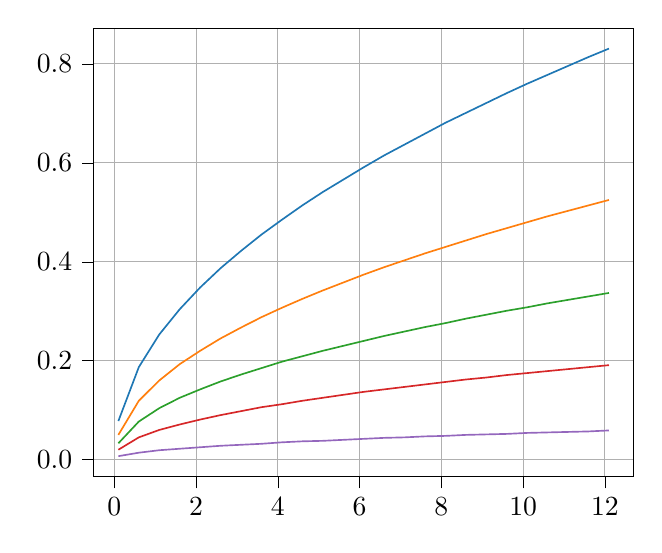
\begin{tikzpicture}

\definecolor{crimson2143940}{RGB}{214,39,40}
\definecolor{darkgray176}{RGB}{176,176,176}
\definecolor{darkorange25512714}{RGB}{255,127,14}
\definecolor{forestgreen4416044}{RGB}{44,160,44}
\definecolor{mediumpurple148103189}{RGB}{148,103,189}
\definecolor{steelblue31119180}{RGB}{31,119,180}

\begin{axis}[
tick align=outside,
tick pos=left,
x grid style={darkgray176},
xmajorgrids,
xmin=-0.5, xmax=12.7,
xtick style={color=black},
xtick={-2,0,2,4,6,8,10,12,14},
xticklabels={
  \(\displaystyle {\ensuremath{-}2}\),
  \(\displaystyle {0}\),
  \(\displaystyle {2}\),
  \(\displaystyle {4}\),
  \(\displaystyle {6}\),
  \(\displaystyle {8}\),
  \(\displaystyle {10}\),
  \(\displaystyle {12}\),
  \(\displaystyle {14}\)
},
y grid style={darkgray176},
ymajorgrids,
ymin=-0.0342, ymax=0.8722,
ytick style={color=black},
ytick={-0.2,0,0.2,0.4,0.6,0.8,1},
yticklabels={
  \(\displaystyle {\ensuremath{-}0.2}\),
  \(\displaystyle {0.0}\),
  \(\displaystyle {0.2}\),
  \(\displaystyle {0.4}\),
  \(\displaystyle {0.6}\),
  \(\displaystyle {0.8}\),
  \(\displaystyle {1.0}\)
}
]
\addplot [semithick, steelblue31119180]
table {%
0.1 0.078
0.6 0.187
1.1 0.253
1.6 0.304
2.1 0.348
2.6 0.387
3.1 0.422
3.6 0.455
4.1 0.485
4.6 0.514
5.1 0.541
5.6 0.566
6.1 0.591
6.6 0.615
7.1 0.637
7.6 0.659
8.1 0.681
8.6 0.701
9.1 0.721
9.6 0.741
10.1 0.76
10.6 0.778
11.1 0.796
11.6 0.814
12.1 0.831
};
\addplot [semithick, darkorange25512714]
table {%
0.1 0.05
0.6 0.119
1.1 0.16
1.6 0.193
2.1 0.22
2.6 0.245
3.1 0.267
3.6 0.288
4.1 0.307
4.6 0.325
5.1 0.342
5.6 0.358
6.1 0.374
6.6 0.389
7.1 0.403
7.6 0.417
8.1 0.43
8.6 0.443
9.1 0.456
9.6 0.468
10.1 0.48
10.6 0.492
11.1 0.503
11.6 0.514
12.1 0.525
};
\addplot [semithick, forestgreen4416044]
table {%
0.1 0.033
0.6 0.077
1.1 0.104
1.6 0.125
2.1 0.142
2.6 0.158
3.1 0.172
3.6 0.185
4.1 0.198
4.6 0.209
5.1 0.22
5.6 0.23
6.1 0.24
6.6 0.25
7.1 0.259
7.6 0.268
8.1 0.276
8.6 0.285
9.1 0.293
9.6 0.301
10.1 0.308
10.6 0.316
11.1 0.323
11.6 0.33
12.1 0.337
};
\addplot [semithick, crimson2143940]
table {%
0.1 0.02
0.6 0.045
1.1 0.06
1.6 0.071
2.1 0.081
2.6 0.09
3.1 0.098
3.6 0.106
4.1 0.112
4.6 0.119
5.1 0.125
5.6 0.131
6.1 0.137
6.6 0.142
7.1 0.147
7.6 0.152
8.1 0.157
8.6 0.162
9.1 0.166
9.6 0.171
10.1 0.175
10.6 0.179
11.1 0.183
11.6 0.187
12.1 0.191
};
\addplot [semithick, mediumpurple148103189]
table {%
0.1 0.007
0.6 0.014
1.1 0.019
1.6 0.022
2.1 0.025
2.6 0.028
3.1 0.03
3.6 0.032
4.1 0.035
4.6 0.037
5.1 0.038
5.6 0.04
6.1 0.042
6.6 0.044
7.1 0.045
7.6 0.047
8.1 0.048
8.6 0.05
9.1 0.051
9.6 0.052
10.1 0.054
10.6 0.055
11.1 0.056
11.6 0.057
12.1 0.059
};
\end{axis}

\end{tikzpicture}

        %% Creator: Matplotlib, PGF backend
%%
%% To include the figure in your LaTeX document, write
%%   \input{<filename>.pgf}
%%
%% Make sure the required packages are loaded in your preamble
%%   \usepackage{pgf}
%%
%% Also ensure that all the required font packages are loaded; for instance,
%% the lmodern package is sometimes necessary when using math font.
%%   \usepackage{lmodern}
%%
%% Figures using additional raster images can only be included by \input if
%% they are in the same directory as the main LaTeX file. For loading figures
%% from other directories you can use the `import` package
%%   \usepackage{import}
%%
%% and then include the figures with
%%   \import{<path to file>}{<filename>.pgf}
%%
%% Matplotlib used the following preamble
%%   
%%   \usepackage{fontspec}
%%   \setmainfont{Charter.ttc}[Path=\detokenize{/System/Library/Fonts/Supplemental/}]
%%   \setsansfont{DejaVuSans.ttf}[Path=\detokenize{/opt/homebrew/lib/python3.10/site-packages/matplotlib/mpl-data/fonts/ttf/}]
%%   \setmonofont{DejaVuSansMono.ttf}[Path=\detokenize{/opt/homebrew/lib/python3.10/site-packages/matplotlib/mpl-data/fonts/ttf/}]
%%   \makeatletter\@ifpackageloaded{underscore}{}{\usepackage[strings]{underscore}}\makeatother
%%
\begingroup%
\makeatletter%
\begin{pgfpicture}%
\pgfpathrectangle{\pgfpointorigin}{\pgfqpoint{6.400000in}{4.800000in}}%
\pgfusepath{use as bounding box, clip}%
\begin{pgfscope}%
\pgfsetbuttcap%
\pgfsetmiterjoin%
\definecolor{currentfill}{rgb}{1.000000,1.000000,1.000000}%
\pgfsetfillcolor{currentfill}%
\pgfsetlinewidth{0.000000pt}%
\definecolor{currentstroke}{rgb}{1.000000,1.000000,1.000000}%
\pgfsetstrokecolor{currentstroke}%
\pgfsetdash{}{0pt}%
\pgfpathmoveto{\pgfqpoint{0.000000in}{0.000000in}}%
\pgfpathlineto{\pgfqpoint{6.400000in}{0.000000in}}%
\pgfpathlineto{\pgfqpoint{6.400000in}{4.800000in}}%
\pgfpathlineto{\pgfqpoint{0.000000in}{4.800000in}}%
\pgfpathlineto{\pgfqpoint{0.000000in}{0.000000in}}%
\pgfpathclose%
\pgfusepath{fill}%
\end{pgfscope}%
\begin{pgfscope}%
\pgfsetbuttcap%
\pgfsetmiterjoin%
\definecolor{currentfill}{rgb}{1.000000,1.000000,1.000000}%
\pgfsetfillcolor{currentfill}%
\pgfsetlinewidth{0.000000pt}%
\definecolor{currentstroke}{rgb}{0.000000,0.000000,0.000000}%
\pgfsetstrokecolor{currentstroke}%
\pgfsetstrokeopacity{0.000000}%
\pgfsetdash{}{0pt}%
\pgfpathmoveto{\pgfqpoint{0.800000in}{0.528000in}}%
\pgfpathlineto{\pgfqpoint{5.760000in}{0.528000in}}%
\pgfpathlineto{\pgfqpoint{5.760000in}{4.224000in}}%
\pgfpathlineto{\pgfqpoint{0.800000in}{4.224000in}}%
\pgfpathlineto{\pgfqpoint{0.800000in}{0.528000in}}%
\pgfpathclose%
\pgfusepath{fill}%
\end{pgfscope}%
\begin{pgfscope}%
\pgfpathrectangle{\pgfqpoint{0.800000in}{0.528000in}}{\pgfqpoint{4.960000in}{3.696000in}}%
\pgfusepath{clip}%
\pgfsetrectcap%
\pgfsetroundjoin%
\pgfsetlinewidth{0.803000pt}%
\definecolor{currentstroke}{rgb}{0.690196,0.690196,0.690196}%
\pgfsetstrokecolor{currentstroke}%
\pgfsetdash{}{0pt}%
\pgfpathmoveto{\pgfqpoint{0.987879in}{0.528000in}}%
\pgfpathlineto{\pgfqpoint{0.987879in}{4.224000in}}%
\pgfusepath{stroke}%
\end{pgfscope}%
\begin{pgfscope}%
\pgfsetbuttcap%
\pgfsetroundjoin%
\definecolor{currentfill}{rgb}{0.000000,0.000000,0.000000}%
\pgfsetfillcolor{currentfill}%
\pgfsetlinewidth{0.803000pt}%
\definecolor{currentstroke}{rgb}{0.000000,0.000000,0.000000}%
\pgfsetstrokecolor{currentstroke}%
\pgfsetdash{}{0pt}%
\pgfsys@defobject{currentmarker}{\pgfqpoint{0.000000in}{-0.048611in}}{\pgfqpoint{0.000000in}{0.000000in}}{%
\pgfpathmoveto{\pgfqpoint{0.000000in}{0.000000in}}%
\pgfpathlineto{\pgfqpoint{0.000000in}{-0.048611in}}%
\pgfusepath{stroke,fill}%
}%
\begin{pgfscope}%
\pgfsys@transformshift{0.987879in}{0.528000in}%
\pgfsys@useobject{currentmarker}{}%
\end{pgfscope}%
\end{pgfscope}%
\begin{pgfscope}%
\definecolor{textcolor}{rgb}{0.000000,0.000000,0.000000}%
\pgfsetstrokecolor{textcolor}%
\pgfsetfillcolor{textcolor}%
\pgftext[x=0.987879in,y=0.430778in,,top]{\color{textcolor}\rmfamily\fontsize{12.000000}{14.400000}\selectfont \(\displaystyle {0}\)}%
\end{pgfscope}%
\begin{pgfscope}%
\pgfpathrectangle{\pgfqpoint{0.800000in}{0.528000in}}{\pgfqpoint{4.960000in}{3.696000in}}%
\pgfusepath{clip}%
\pgfsetrectcap%
\pgfsetroundjoin%
\pgfsetlinewidth{0.803000pt}%
\definecolor{currentstroke}{rgb}{0.690196,0.690196,0.690196}%
\pgfsetstrokecolor{currentstroke}%
\pgfsetdash{}{0pt}%
\pgfpathmoveto{\pgfqpoint{1.739394in}{0.528000in}}%
\pgfpathlineto{\pgfqpoint{1.739394in}{4.224000in}}%
\pgfusepath{stroke}%
\end{pgfscope}%
\begin{pgfscope}%
\pgfsetbuttcap%
\pgfsetroundjoin%
\definecolor{currentfill}{rgb}{0.000000,0.000000,0.000000}%
\pgfsetfillcolor{currentfill}%
\pgfsetlinewidth{0.803000pt}%
\definecolor{currentstroke}{rgb}{0.000000,0.000000,0.000000}%
\pgfsetstrokecolor{currentstroke}%
\pgfsetdash{}{0pt}%
\pgfsys@defobject{currentmarker}{\pgfqpoint{0.000000in}{-0.048611in}}{\pgfqpoint{0.000000in}{0.000000in}}{%
\pgfpathmoveto{\pgfqpoint{0.000000in}{0.000000in}}%
\pgfpathlineto{\pgfqpoint{0.000000in}{-0.048611in}}%
\pgfusepath{stroke,fill}%
}%
\begin{pgfscope}%
\pgfsys@transformshift{1.739394in}{0.528000in}%
\pgfsys@useobject{currentmarker}{}%
\end{pgfscope}%
\end{pgfscope}%
\begin{pgfscope}%
\definecolor{textcolor}{rgb}{0.000000,0.000000,0.000000}%
\pgfsetstrokecolor{textcolor}%
\pgfsetfillcolor{textcolor}%
\pgftext[x=1.739394in,y=0.430778in,,top]{\color{textcolor}\rmfamily\fontsize{12.000000}{14.400000}\selectfont \(\displaystyle {2}\)}%
\end{pgfscope}%
\begin{pgfscope}%
\pgfpathrectangle{\pgfqpoint{0.800000in}{0.528000in}}{\pgfqpoint{4.960000in}{3.696000in}}%
\pgfusepath{clip}%
\pgfsetrectcap%
\pgfsetroundjoin%
\pgfsetlinewidth{0.803000pt}%
\definecolor{currentstroke}{rgb}{0.690196,0.690196,0.690196}%
\pgfsetstrokecolor{currentstroke}%
\pgfsetdash{}{0pt}%
\pgfpathmoveto{\pgfqpoint{2.490909in}{0.528000in}}%
\pgfpathlineto{\pgfqpoint{2.490909in}{4.224000in}}%
\pgfusepath{stroke}%
\end{pgfscope}%
\begin{pgfscope}%
\pgfsetbuttcap%
\pgfsetroundjoin%
\definecolor{currentfill}{rgb}{0.000000,0.000000,0.000000}%
\pgfsetfillcolor{currentfill}%
\pgfsetlinewidth{0.803000pt}%
\definecolor{currentstroke}{rgb}{0.000000,0.000000,0.000000}%
\pgfsetstrokecolor{currentstroke}%
\pgfsetdash{}{0pt}%
\pgfsys@defobject{currentmarker}{\pgfqpoint{0.000000in}{-0.048611in}}{\pgfqpoint{0.000000in}{0.000000in}}{%
\pgfpathmoveto{\pgfqpoint{0.000000in}{0.000000in}}%
\pgfpathlineto{\pgfqpoint{0.000000in}{-0.048611in}}%
\pgfusepath{stroke,fill}%
}%
\begin{pgfscope}%
\pgfsys@transformshift{2.490909in}{0.528000in}%
\pgfsys@useobject{currentmarker}{}%
\end{pgfscope}%
\end{pgfscope}%
\begin{pgfscope}%
\definecolor{textcolor}{rgb}{0.000000,0.000000,0.000000}%
\pgfsetstrokecolor{textcolor}%
\pgfsetfillcolor{textcolor}%
\pgftext[x=2.490909in,y=0.430778in,,top]{\color{textcolor}\rmfamily\fontsize{12.000000}{14.400000}\selectfont \(\displaystyle {4}\)}%
\end{pgfscope}%
\begin{pgfscope}%
\pgfpathrectangle{\pgfqpoint{0.800000in}{0.528000in}}{\pgfqpoint{4.960000in}{3.696000in}}%
\pgfusepath{clip}%
\pgfsetrectcap%
\pgfsetroundjoin%
\pgfsetlinewidth{0.803000pt}%
\definecolor{currentstroke}{rgb}{0.690196,0.690196,0.690196}%
\pgfsetstrokecolor{currentstroke}%
\pgfsetdash{}{0pt}%
\pgfpathmoveto{\pgfqpoint{3.242424in}{0.528000in}}%
\pgfpathlineto{\pgfqpoint{3.242424in}{4.224000in}}%
\pgfusepath{stroke}%
\end{pgfscope}%
\begin{pgfscope}%
\pgfsetbuttcap%
\pgfsetroundjoin%
\definecolor{currentfill}{rgb}{0.000000,0.000000,0.000000}%
\pgfsetfillcolor{currentfill}%
\pgfsetlinewidth{0.803000pt}%
\definecolor{currentstroke}{rgb}{0.000000,0.000000,0.000000}%
\pgfsetstrokecolor{currentstroke}%
\pgfsetdash{}{0pt}%
\pgfsys@defobject{currentmarker}{\pgfqpoint{0.000000in}{-0.048611in}}{\pgfqpoint{0.000000in}{0.000000in}}{%
\pgfpathmoveto{\pgfqpoint{0.000000in}{0.000000in}}%
\pgfpathlineto{\pgfqpoint{0.000000in}{-0.048611in}}%
\pgfusepath{stroke,fill}%
}%
\begin{pgfscope}%
\pgfsys@transformshift{3.242424in}{0.528000in}%
\pgfsys@useobject{currentmarker}{}%
\end{pgfscope}%
\end{pgfscope}%
\begin{pgfscope}%
\definecolor{textcolor}{rgb}{0.000000,0.000000,0.000000}%
\pgfsetstrokecolor{textcolor}%
\pgfsetfillcolor{textcolor}%
\pgftext[x=3.242424in,y=0.430778in,,top]{\color{textcolor}\rmfamily\fontsize{12.000000}{14.400000}\selectfont \(\displaystyle {6}\)}%
\end{pgfscope}%
\begin{pgfscope}%
\pgfpathrectangle{\pgfqpoint{0.800000in}{0.528000in}}{\pgfqpoint{4.960000in}{3.696000in}}%
\pgfusepath{clip}%
\pgfsetrectcap%
\pgfsetroundjoin%
\pgfsetlinewidth{0.803000pt}%
\definecolor{currentstroke}{rgb}{0.690196,0.690196,0.690196}%
\pgfsetstrokecolor{currentstroke}%
\pgfsetdash{}{0pt}%
\pgfpathmoveto{\pgfqpoint{3.993939in}{0.528000in}}%
\pgfpathlineto{\pgfqpoint{3.993939in}{4.224000in}}%
\pgfusepath{stroke}%
\end{pgfscope}%
\begin{pgfscope}%
\pgfsetbuttcap%
\pgfsetroundjoin%
\definecolor{currentfill}{rgb}{0.000000,0.000000,0.000000}%
\pgfsetfillcolor{currentfill}%
\pgfsetlinewidth{0.803000pt}%
\definecolor{currentstroke}{rgb}{0.000000,0.000000,0.000000}%
\pgfsetstrokecolor{currentstroke}%
\pgfsetdash{}{0pt}%
\pgfsys@defobject{currentmarker}{\pgfqpoint{0.000000in}{-0.048611in}}{\pgfqpoint{0.000000in}{0.000000in}}{%
\pgfpathmoveto{\pgfqpoint{0.000000in}{0.000000in}}%
\pgfpathlineto{\pgfqpoint{0.000000in}{-0.048611in}}%
\pgfusepath{stroke,fill}%
}%
\begin{pgfscope}%
\pgfsys@transformshift{3.993939in}{0.528000in}%
\pgfsys@useobject{currentmarker}{}%
\end{pgfscope}%
\end{pgfscope}%
\begin{pgfscope}%
\definecolor{textcolor}{rgb}{0.000000,0.000000,0.000000}%
\pgfsetstrokecolor{textcolor}%
\pgfsetfillcolor{textcolor}%
\pgftext[x=3.993939in,y=0.430778in,,top]{\color{textcolor}\rmfamily\fontsize{12.000000}{14.400000}\selectfont \(\displaystyle {8}\)}%
\end{pgfscope}%
\begin{pgfscope}%
\pgfpathrectangle{\pgfqpoint{0.800000in}{0.528000in}}{\pgfqpoint{4.960000in}{3.696000in}}%
\pgfusepath{clip}%
\pgfsetrectcap%
\pgfsetroundjoin%
\pgfsetlinewidth{0.803000pt}%
\definecolor{currentstroke}{rgb}{0.690196,0.690196,0.690196}%
\pgfsetstrokecolor{currentstroke}%
\pgfsetdash{}{0pt}%
\pgfpathmoveto{\pgfqpoint{4.745455in}{0.528000in}}%
\pgfpathlineto{\pgfqpoint{4.745455in}{4.224000in}}%
\pgfusepath{stroke}%
\end{pgfscope}%
\begin{pgfscope}%
\pgfsetbuttcap%
\pgfsetroundjoin%
\definecolor{currentfill}{rgb}{0.000000,0.000000,0.000000}%
\pgfsetfillcolor{currentfill}%
\pgfsetlinewidth{0.803000pt}%
\definecolor{currentstroke}{rgb}{0.000000,0.000000,0.000000}%
\pgfsetstrokecolor{currentstroke}%
\pgfsetdash{}{0pt}%
\pgfsys@defobject{currentmarker}{\pgfqpoint{0.000000in}{-0.048611in}}{\pgfqpoint{0.000000in}{0.000000in}}{%
\pgfpathmoveto{\pgfqpoint{0.000000in}{0.000000in}}%
\pgfpathlineto{\pgfqpoint{0.000000in}{-0.048611in}}%
\pgfusepath{stroke,fill}%
}%
\begin{pgfscope}%
\pgfsys@transformshift{4.745455in}{0.528000in}%
\pgfsys@useobject{currentmarker}{}%
\end{pgfscope}%
\end{pgfscope}%
\begin{pgfscope}%
\definecolor{textcolor}{rgb}{0.000000,0.000000,0.000000}%
\pgfsetstrokecolor{textcolor}%
\pgfsetfillcolor{textcolor}%
\pgftext[x=4.745455in,y=0.430778in,,top]{\color{textcolor}\rmfamily\fontsize{12.000000}{14.400000}\selectfont \(\displaystyle {10}\)}%
\end{pgfscope}%
\begin{pgfscope}%
\pgfpathrectangle{\pgfqpoint{0.800000in}{0.528000in}}{\pgfqpoint{4.960000in}{3.696000in}}%
\pgfusepath{clip}%
\pgfsetrectcap%
\pgfsetroundjoin%
\pgfsetlinewidth{0.803000pt}%
\definecolor{currentstroke}{rgb}{0.690196,0.690196,0.690196}%
\pgfsetstrokecolor{currentstroke}%
\pgfsetdash{}{0pt}%
\pgfpathmoveto{\pgfqpoint{5.496970in}{0.528000in}}%
\pgfpathlineto{\pgfqpoint{5.496970in}{4.224000in}}%
\pgfusepath{stroke}%
\end{pgfscope}%
\begin{pgfscope}%
\pgfsetbuttcap%
\pgfsetroundjoin%
\definecolor{currentfill}{rgb}{0.000000,0.000000,0.000000}%
\pgfsetfillcolor{currentfill}%
\pgfsetlinewidth{0.803000pt}%
\definecolor{currentstroke}{rgb}{0.000000,0.000000,0.000000}%
\pgfsetstrokecolor{currentstroke}%
\pgfsetdash{}{0pt}%
\pgfsys@defobject{currentmarker}{\pgfqpoint{0.000000in}{-0.048611in}}{\pgfqpoint{0.000000in}{0.000000in}}{%
\pgfpathmoveto{\pgfqpoint{0.000000in}{0.000000in}}%
\pgfpathlineto{\pgfqpoint{0.000000in}{-0.048611in}}%
\pgfusepath{stroke,fill}%
}%
\begin{pgfscope}%
\pgfsys@transformshift{5.496970in}{0.528000in}%
\pgfsys@useobject{currentmarker}{}%
\end{pgfscope}%
\end{pgfscope}%
\begin{pgfscope}%
\definecolor{textcolor}{rgb}{0.000000,0.000000,0.000000}%
\pgfsetstrokecolor{textcolor}%
\pgfsetfillcolor{textcolor}%
\pgftext[x=5.496970in,y=0.430778in,,top]{\color{textcolor}\rmfamily\fontsize{12.000000}{14.400000}\selectfont \(\displaystyle {12}\)}%
\end{pgfscope}%
\begin{pgfscope}%
\definecolor{textcolor}{rgb}{0.000000,0.000000,0.000000}%
\pgfsetstrokecolor{textcolor}%
\pgfsetfillcolor{textcolor}%
\pgftext[x=3.280000in,y=0.216287in,,top]{\color{textcolor}\rmfamily\fontsize{12.000000}{14.400000}\selectfont \(\displaystyle H_\mathrm{gen}\) in \(\displaystyle \mathrm{s}\)}%
\end{pgfscope}%
\begin{pgfscope}%
\pgfpathrectangle{\pgfqpoint{0.800000in}{0.528000in}}{\pgfqpoint{4.960000in}{3.696000in}}%
\pgfusepath{clip}%
\pgfsetrectcap%
\pgfsetroundjoin%
\pgfsetlinewidth{0.803000pt}%
\definecolor{currentstroke}{rgb}{0.690196,0.690196,0.690196}%
\pgfsetstrokecolor{currentstroke}%
\pgfsetdash{}{0pt}%
\pgfpathmoveto{\pgfqpoint{0.800000in}{0.667456in}}%
\pgfpathlineto{\pgfqpoint{5.760000in}{0.667456in}}%
\pgfusepath{stroke}%
\end{pgfscope}%
\begin{pgfscope}%
\pgfsetbuttcap%
\pgfsetroundjoin%
\definecolor{currentfill}{rgb}{0.000000,0.000000,0.000000}%
\pgfsetfillcolor{currentfill}%
\pgfsetlinewidth{0.803000pt}%
\definecolor{currentstroke}{rgb}{0.000000,0.000000,0.000000}%
\pgfsetstrokecolor{currentstroke}%
\pgfsetdash{}{0pt}%
\pgfsys@defobject{currentmarker}{\pgfqpoint{-0.048611in}{0.000000in}}{\pgfqpoint{-0.000000in}{0.000000in}}{%
\pgfpathmoveto{\pgfqpoint{-0.000000in}{0.000000in}}%
\pgfpathlineto{\pgfqpoint{-0.048611in}{0.000000in}}%
\pgfusepath{stroke,fill}%
}%
\begin{pgfscope}%
\pgfsys@transformshift{0.800000in}{0.667456in}%
\pgfsys@useobject{currentmarker}{}%
\end{pgfscope}%
\end{pgfscope}%
\begin{pgfscope}%
\definecolor{textcolor}{rgb}{0.000000,0.000000,0.000000}%
\pgfsetstrokecolor{textcolor}%
\pgfsetfillcolor{textcolor}%
\pgftext[x=0.494254in, y=0.606136in, left, base]{\color{textcolor}\rmfamily\fontsize{12.000000}{14.400000}\selectfont \(\displaystyle {0.0}\)}%
\end{pgfscope}%
\begin{pgfscope}%
\pgfpathrectangle{\pgfqpoint{0.800000in}{0.528000in}}{\pgfqpoint{4.960000in}{3.696000in}}%
\pgfusepath{clip}%
\pgfsetrectcap%
\pgfsetroundjoin%
\pgfsetlinewidth{0.803000pt}%
\definecolor{currentstroke}{rgb}{0.690196,0.690196,0.690196}%
\pgfsetstrokecolor{currentstroke}%
\pgfsetdash{}{0pt}%
\pgfpathmoveto{\pgfqpoint{0.800000in}{1.482990in}}%
\pgfpathlineto{\pgfqpoint{5.760000in}{1.482990in}}%
\pgfusepath{stroke}%
\end{pgfscope}%
\begin{pgfscope}%
\pgfsetbuttcap%
\pgfsetroundjoin%
\definecolor{currentfill}{rgb}{0.000000,0.000000,0.000000}%
\pgfsetfillcolor{currentfill}%
\pgfsetlinewidth{0.803000pt}%
\definecolor{currentstroke}{rgb}{0.000000,0.000000,0.000000}%
\pgfsetstrokecolor{currentstroke}%
\pgfsetdash{}{0pt}%
\pgfsys@defobject{currentmarker}{\pgfqpoint{-0.048611in}{0.000000in}}{\pgfqpoint{-0.000000in}{0.000000in}}{%
\pgfpathmoveto{\pgfqpoint{-0.000000in}{0.000000in}}%
\pgfpathlineto{\pgfqpoint{-0.048611in}{0.000000in}}%
\pgfusepath{stroke,fill}%
}%
\begin{pgfscope}%
\pgfsys@transformshift{0.800000in}{1.482990in}%
\pgfsys@useobject{currentmarker}{}%
\end{pgfscope}%
\end{pgfscope}%
\begin{pgfscope}%
\definecolor{textcolor}{rgb}{0.000000,0.000000,0.000000}%
\pgfsetstrokecolor{textcolor}%
\pgfsetfillcolor{textcolor}%
\pgftext[x=0.494254in, y=1.421670in, left, base]{\color{textcolor}\rmfamily\fontsize{12.000000}{14.400000}\selectfont \(\displaystyle {0.2}\)}%
\end{pgfscope}%
\begin{pgfscope}%
\pgfpathrectangle{\pgfqpoint{0.800000in}{0.528000in}}{\pgfqpoint{4.960000in}{3.696000in}}%
\pgfusepath{clip}%
\pgfsetrectcap%
\pgfsetroundjoin%
\pgfsetlinewidth{0.803000pt}%
\definecolor{currentstroke}{rgb}{0.690196,0.690196,0.690196}%
\pgfsetstrokecolor{currentstroke}%
\pgfsetdash{}{0pt}%
\pgfpathmoveto{\pgfqpoint{0.800000in}{2.298524in}}%
\pgfpathlineto{\pgfqpoint{5.760000in}{2.298524in}}%
\pgfusepath{stroke}%
\end{pgfscope}%
\begin{pgfscope}%
\pgfsetbuttcap%
\pgfsetroundjoin%
\definecolor{currentfill}{rgb}{0.000000,0.000000,0.000000}%
\pgfsetfillcolor{currentfill}%
\pgfsetlinewidth{0.803000pt}%
\definecolor{currentstroke}{rgb}{0.000000,0.000000,0.000000}%
\pgfsetstrokecolor{currentstroke}%
\pgfsetdash{}{0pt}%
\pgfsys@defobject{currentmarker}{\pgfqpoint{-0.048611in}{0.000000in}}{\pgfqpoint{-0.000000in}{0.000000in}}{%
\pgfpathmoveto{\pgfqpoint{-0.000000in}{0.000000in}}%
\pgfpathlineto{\pgfqpoint{-0.048611in}{0.000000in}}%
\pgfusepath{stroke,fill}%
}%
\begin{pgfscope}%
\pgfsys@transformshift{0.800000in}{2.298524in}%
\pgfsys@useobject{currentmarker}{}%
\end{pgfscope}%
\end{pgfscope}%
\begin{pgfscope}%
\definecolor{textcolor}{rgb}{0.000000,0.000000,0.000000}%
\pgfsetstrokecolor{textcolor}%
\pgfsetfillcolor{textcolor}%
\pgftext[x=0.494254in, y=2.237204in, left, base]{\color{textcolor}\rmfamily\fontsize{12.000000}{14.400000}\selectfont \(\displaystyle {0.4}\)}%
\end{pgfscope}%
\begin{pgfscope}%
\pgfpathrectangle{\pgfqpoint{0.800000in}{0.528000in}}{\pgfqpoint{4.960000in}{3.696000in}}%
\pgfusepath{clip}%
\pgfsetrectcap%
\pgfsetroundjoin%
\pgfsetlinewidth{0.803000pt}%
\definecolor{currentstroke}{rgb}{0.690196,0.690196,0.690196}%
\pgfsetstrokecolor{currentstroke}%
\pgfsetdash{}{0pt}%
\pgfpathmoveto{\pgfqpoint{0.800000in}{3.114058in}}%
\pgfpathlineto{\pgfqpoint{5.760000in}{3.114058in}}%
\pgfusepath{stroke}%
\end{pgfscope}%
\begin{pgfscope}%
\pgfsetbuttcap%
\pgfsetroundjoin%
\definecolor{currentfill}{rgb}{0.000000,0.000000,0.000000}%
\pgfsetfillcolor{currentfill}%
\pgfsetlinewidth{0.803000pt}%
\definecolor{currentstroke}{rgb}{0.000000,0.000000,0.000000}%
\pgfsetstrokecolor{currentstroke}%
\pgfsetdash{}{0pt}%
\pgfsys@defobject{currentmarker}{\pgfqpoint{-0.048611in}{0.000000in}}{\pgfqpoint{-0.000000in}{0.000000in}}{%
\pgfpathmoveto{\pgfqpoint{-0.000000in}{0.000000in}}%
\pgfpathlineto{\pgfqpoint{-0.048611in}{0.000000in}}%
\pgfusepath{stroke,fill}%
}%
\begin{pgfscope}%
\pgfsys@transformshift{0.800000in}{3.114058in}%
\pgfsys@useobject{currentmarker}{}%
\end{pgfscope}%
\end{pgfscope}%
\begin{pgfscope}%
\definecolor{textcolor}{rgb}{0.000000,0.000000,0.000000}%
\pgfsetstrokecolor{textcolor}%
\pgfsetfillcolor{textcolor}%
\pgftext[x=0.494254in, y=3.052738in, left, base]{\color{textcolor}\rmfamily\fontsize{12.000000}{14.400000}\selectfont \(\displaystyle {0.6}\)}%
\end{pgfscope}%
\begin{pgfscope}%
\pgfpathrectangle{\pgfqpoint{0.800000in}{0.528000in}}{\pgfqpoint{4.960000in}{3.696000in}}%
\pgfusepath{clip}%
\pgfsetrectcap%
\pgfsetroundjoin%
\pgfsetlinewidth{0.803000pt}%
\definecolor{currentstroke}{rgb}{0.690196,0.690196,0.690196}%
\pgfsetstrokecolor{currentstroke}%
\pgfsetdash{}{0pt}%
\pgfpathmoveto{\pgfqpoint{0.800000in}{3.929592in}}%
\pgfpathlineto{\pgfqpoint{5.760000in}{3.929592in}}%
\pgfusepath{stroke}%
\end{pgfscope}%
\begin{pgfscope}%
\pgfsetbuttcap%
\pgfsetroundjoin%
\definecolor{currentfill}{rgb}{0.000000,0.000000,0.000000}%
\pgfsetfillcolor{currentfill}%
\pgfsetlinewidth{0.803000pt}%
\definecolor{currentstroke}{rgb}{0.000000,0.000000,0.000000}%
\pgfsetstrokecolor{currentstroke}%
\pgfsetdash{}{0pt}%
\pgfsys@defobject{currentmarker}{\pgfqpoint{-0.048611in}{0.000000in}}{\pgfqpoint{-0.000000in}{0.000000in}}{%
\pgfpathmoveto{\pgfqpoint{-0.000000in}{0.000000in}}%
\pgfpathlineto{\pgfqpoint{-0.048611in}{0.000000in}}%
\pgfusepath{stroke,fill}%
}%
\begin{pgfscope}%
\pgfsys@transformshift{0.800000in}{3.929592in}%
\pgfsys@useobject{currentmarker}{}%
\end{pgfscope}%
\end{pgfscope}%
\begin{pgfscope}%
\definecolor{textcolor}{rgb}{0.000000,0.000000,0.000000}%
\pgfsetstrokecolor{textcolor}%
\pgfsetfillcolor{textcolor}%
\pgftext[x=0.494254in, y=3.868272in, left, base]{\color{textcolor}\rmfamily\fontsize{12.000000}{14.400000}\selectfont \(\displaystyle {0.8}\)}%
\end{pgfscope}%
\begin{pgfscope}%
\definecolor{textcolor}{rgb}{0.000000,0.000000,0.000000}%
\pgfsetstrokecolor{textcolor}%
\pgfsetfillcolor{textcolor}%
\pgftext[x=0.438698in,y=2.376000in,,bottom,rotate=90.000000]{\color{textcolor}\rmfamily\fontsize{12.000000}{14.400000}\selectfont \(\displaystyle CCT\) in \(\displaystyle \mathrm{s}\)}%
\end{pgfscope}%
\begin{pgfscope}%
\pgfpathrectangle{\pgfqpoint{0.800000in}{0.528000in}}{\pgfqpoint{4.960000in}{3.696000in}}%
\pgfusepath{clip}%
\pgfsetrectcap%
\pgfsetroundjoin%
\pgfsetlinewidth{1.505625pt}%
\definecolor{currentstroke}{rgb}{0.121569,0.466667,0.705882}%
\pgfsetstrokecolor{currentstroke}%
\pgfsetdash{}{0pt}%
\pgfpathmoveto{\pgfqpoint{1.025455in}{0.985515in}}%
\pgfpathlineto{\pgfqpoint{1.213333in}{1.429981in}}%
\pgfpathlineto{\pgfqpoint{1.401212in}{1.699107in}}%
\pgfpathlineto{\pgfqpoint{1.589091in}{1.907068in}}%
\pgfpathlineto{\pgfqpoint{1.776970in}{2.086485in}}%
\pgfpathlineto{\pgfqpoint{1.964848in}{2.245515in}}%
\pgfpathlineto{\pgfqpoint{2.152727in}{2.388233in}}%
\pgfpathlineto{\pgfqpoint{2.340606in}{2.522796in}}%
\pgfpathlineto{\pgfqpoint{2.528485in}{2.645126in}}%
\pgfpathlineto{\pgfqpoint{2.716364in}{2.763379in}}%
\pgfpathlineto{\pgfqpoint{2.904242in}{2.873476in}}%
\pgfpathlineto{\pgfqpoint{3.092121in}{2.975417in}}%
\pgfpathlineto{\pgfqpoint{3.280000in}{3.077359in}}%
\pgfpathlineto{\pgfqpoint{3.467879in}{3.175223in}}%
\pgfpathlineto{\pgfqpoint{3.655758in}{3.264932in}}%
\pgfpathlineto{\pgfqpoint{3.843636in}{3.354641in}}%
\pgfpathlineto{\pgfqpoint{4.031515in}{3.444350in}}%
\pgfpathlineto{\pgfqpoint{4.219394in}{3.525903in}}%
\pgfpathlineto{\pgfqpoint{4.407273in}{3.607456in}}%
\pgfpathlineto{\pgfqpoint{4.595152in}{3.689010in}}%
\pgfpathlineto{\pgfqpoint{4.783030in}{3.766485in}}%
\pgfpathlineto{\pgfqpoint{4.970909in}{3.839883in}}%
\pgfpathlineto{\pgfqpoint{5.158788in}{3.913282in}}%
\pgfpathlineto{\pgfqpoint{5.346667in}{3.986680in}}%
\pgfpathlineto{\pgfqpoint{5.534545in}{4.056000in}}%
\pgfusepath{stroke}%
\end{pgfscope}%
\begin{pgfscope}%
\pgfpathrectangle{\pgfqpoint{0.800000in}{0.528000in}}{\pgfqpoint{4.960000in}{3.696000in}}%
\pgfusepath{clip}%
\pgfsetrectcap%
\pgfsetroundjoin%
\pgfsetlinewidth{1.505625pt}%
\definecolor{currentstroke}{rgb}{1.000000,0.498039,0.054902}%
\pgfsetstrokecolor{currentstroke}%
\pgfsetdash{}{0pt}%
\pgfpathmoveto{\pgfqpoint{1.025455in}{0.871340in}}%
\pgfpathlineto{\pgfqpoint{1.213333in}{1.152699in}}%
\pgfpathlineto{\pgfqpoint{1.401212in}{1.319883in}}%
\pgfpathlineto{\pgfqpoint{1.589091in}{1.454447in}}%
\pgfpathlineto{\pgfqpoint{1.776970in}{1.564544in}}%
\pgfpathlineto{\pgfqpoint{1.964848in}{1.666485in}}%
\pgfpathlineto{\pgfqpoint{2.152727in}{1.756194in}}%
\pgfpathlineto{\pgfqpoint{2.340606in}{1.841825in}}%
\pgfpathlineto{\pgfqpoint{2.528485in}{1.919301in}}%
\pgfpathlineto{\pgfqpoint{2.716364in}{1.992699in}}%
\pgfpathlineto{\pgfqpoint{2.904242in}{2.062019in}}%
\pgfpathlineto{\pgfqpoint{3.092121in}{2.127262in}}%
\pgfpathlineto{\pgfqpoint{3.280000in}{2.192505in}}%
\pgfpathlineto{\pgfqpoint{3.467879in}{2.253670in}}%
\pgfpathlineto{\pgfqpoint{3.655758in}{2.310757in}}%
\pgfpathlineto{\pgfqpoint{3.843636in}{2.367845in}}%
\pgfpathlineto{\pgfqpoint{4.031515in}{2.420854in}}%
\pgfpathlineto{\pgfqpoint{4.219394in}{2.473864in}}%
\pgfpathlineto{\pgfqpoint{4.407273in}{2.526874in}}%
\pgfpathlineto{\pgfqpoint{4.595152in}{2.575806in}}%
\pgfpathlineto{\pgfqpoint{4.783030in}{2.624738in}}%
\pgfpathlineto{\pgfqpoint{4.970909in}{2.673670in}}%
\pgfpathlineto{\pgfqpoint{5.158788in}{2.718524in}}%
\pgfpathlineto{\pgfqpoint{5.346667in}{2.763379in}}%
\pgfpathlineto{\pgfqpoint{5.534545in}{2.808233in}}%
\pgfusepath{stroke}%
\end{pgfscope}%
\begin{pgfscope}%
\pgfpathrectangle{\pgfqpoint{0.800000in}{0.528000in}}{\pgfqpoint{4.960000in}{3.696000in}}%
\pgfusepath{clip}%
\pgfsetrectcap%
\pgfsetroundjoin%
\pgfsetlinewidth{1.505625pt}%
\definecolor{currentstroke}{rgb}{0.172549,0.627451,0.172549}%
\pgfsetstrokecolor{currentstroke}%
\pgfsetdash{}{0pt}%
\pgfpathmoveto{\pgfqpoint{1.025455in}{0.802019in}}%
\pgfpathlineto{\pgfqpoint{1.213333in}{0.981437in}}%
\pgfpathlineto{\pgfqpoint{1.401212in}{1.091534in}}%
\pgfpathlineto{\pgfqpoint{1.589091in}{1.177165in}}%
\pgfpathlineto{\pgfqpoint{1.776970in}{1.246485in}}%
\pgfpathlineto{\pgfqpoint{1.964848in}{1.311728in}}%
\pgfpathlineto{\pgfqpoint{2.152727in}{1.368816in}}%
\pgfpathlineto{\pgfqpoint{2.340606in}{1.421825in}}%
\pgfpathlineto{\pgfqpoint{2.528485in}{1.474835in}}%
\pgfpathlineto{\pgfqpoint{2.716364in}{1.519689in}}%
\pgfpathlineto{\pgfqpoint{2.904242in}{1.564544in}}%
\pgfpathlineto{\pgfqpoint{3.092121in}{1.605320in}}%
\pgfpathlineto{\pgfqpoint{3.280000in}{1.646097in}}%
\pgfpathlineto{\pgfqpoint{3.467879in}{1.686874in}}%
\pgfpathlineto{\pgfqpoint{3.655758in}{1.723573in}}%
\pgfpathlineto{\pgfqpoint{3.843636in}{1.760272in}}%
\pgfpathlineto{\pgfqpoint{4.031515in}{1.792893in}}%
\pgfpathlineto{\pgfqpoint{4.219394in}{1.829592in}}%
\pgfpathlineto{\pgfqpoint{4.407273in}{1.862214in}}%
\pgfpathlineto{\pgfqpoint{4.595152in}{1.894835in}}%
\pgfpathlineto{\pgfqpoint{4.783030in}{1.923379in}}%
\pgfpathlineto{\pgfqpoint{4.970909in}{1.956000in}}%
\pgfpathlineto{\pgfqpoint{5.158788in}{1.984544in}}%
\pgfpathlineto{\pgfqpoint{5.346667in}{2.013087in}}%
\pgfpathlineto{\pgfqpoint{5.534545in}{2.041631in}}%
\pgfusepath{stroke}%
\end{pgfscope}%
\begin{pgfscope}%
\pgfpathrectangle{\pgfqpoint{0.800000in}{0.528000in}}{\pgfqpoint{4.960000in}{3.696000in}}%
\pgfusepath{clip}%
\pgfsetrectcap%
\pgfsetroundjoin%
\pgfsetlinewidth{1.505625pt}%
\definecolor{currentstroke}{rgb}{0.839216,0.152941,0.156863}%
\pgfsetstrokecolor{currentstroke}%
\pgfsetdash{}{0pt}%
\pgfpathmoveto{\pgfqpoint{1.025455in}{0.749010in}}%
\pgfpathlineto{\pgfqpoint{1.213333in}{0.850951in}}%
\pgfpathlineto{\pgfqpoint{1.401212in}{0.912117in}}%
\pgfpathlineto{\pgfqpoint{1.589091in}{0.956971in}}%
\pgfpathlineto{\pgfqpoint{1.776970in}{0.997748in}}%
\pgfpathlineto{\pgfqpoint{1.964848in}{1.034447in}}%
\pgfpathlineto{\pgfqpoint{2.152727in}{1.067068in}}%
\pgfpathlineto{\pgfqpoint{2.340606in}{1.099689in}}%
\pgfpathlineto{\pgfqpoint{2.528485in}{1.124155in}}%
\pgfpathlineto{\pgfqpoint{2.716364in}{1.152699in}}%
\pgfpathlineto{\pgfqpoint{2.904242in}{1.177165in}}%
\pgfpathlineto{\pgfqpoint{3.092121in}{1.201631in}}%
\pgfpathlineto{\pgfqpoint{3.280000in}{1.226097in}}%
\pgfpathlineto{\pgfqpoint{3.467879in}{1.246485in}}%
\pgfpathlineto{\pgfqpoint{3.655758in}{1.266874in}}%
\pgfpathlineto{\pgfqpoint{3.843636in}{1.287262in}}%
\pgfpathlineto{\pgfqpoint{4.031515in}{1.307650in}}%
\pgfpathlineto{\pgfqpoint{4.219394in}{1.328039in}}%
\pgfpathlineto{\pgfqpoint{4.407273in}{1.344350in}}%
\pgfpathlineto{\pgfqpoint{4.595152in}{1.364738in}}%
\pgfpathlineto{\pgfqpoint{4.783030in}{1.381049in}}%
\pgfpathlineto{\pgfqpoint{4.970909in}{1.397359in}}%
\pgfpathlineto{\pgfqpoint{5.158788in}{1.413670in}}%
\pgfpathlineto{\pgfqpoint{5.346667in}{1.429981in}}%
\pgfpathlineto{\pgfqpoint{5.534545in}{1.446291in}}%
\pgfusepath{stroke}%
\end{pgfscope}%
\begin{pgfscope}%
\pgfpathrectangle{\pgfqpoint{0.800000in}{0.528000in}}{\pgfqpoint{4.960000in}{3.696000in}}%
\pgfusepath{clip}%
\pgfsetrectcap%
\pgfsetroundjoin%
\pgfsetlinewidth{1.505625pt}%
\definecolor{currentstroke}{rgb}{0.580392,0.403922,0.741176}%
\pgfsetstrokecolor{currentstroke}%
\pgfsetdash{}{0pt}%
\pgfpathmoveto{\pgfqpoint{1.025455in}{0.696000in}}%
\pgfpathlineto{\pgfqpoint{1.213333in}{0.724544in}}%
\pgfpathlineto{\pgfqpoint{1.401212in}{0.744932in}}%
\pgfpathlineto{\pgfqpoint{1.589091in}{0.757165in}}%
\pgfpathlineto{\pgfqpoint{1.776970in}{0.769398in}}%
\pgfpathlineto{\pgfqpoint{1.964848in}{0.781631in}}%
\pgfpathlineto{\pgfqpoint{2.152727in}{0.789786in}}%
\pgfpathlineto{\pgfqpoint{2.340606in}{0.797942in}}%
\pgfpathlineto{\pgfqpoint{2.528485in}{0.810175in}}%
\pgfpathlineto{\pgfqpoint{2.716364in}{0.818330in}}%
\pgfpathlineto{\pgfqpoint{2.904242in}{0.822408in}}%
\pgfpathlineto{\pgfqpoint{3.092121in}{0.830563in}}%
\pgfpathlineto{\pgfqpoint{3.280000in}{0.838718in}}%
\pgfpathlineto{\pgfqpoint{3.467879in}{0.846874in}}%
\pgfpathlineto{\pgfqpoint{3.655758in}{0.850951in}}%
\pgfpathlineto{\pgfqpoint{3.843636in}{0.859107in}}%
\pgfpathlineto{\pgfqpoint{4.031515in}{0.863184in}}%
\pgfpathlineto{\pgfqpoint{4.219394in}{0.871340in}}%
\pgfpathlineto{\pgfqpoint{4.407273in}{0.875417in}}%
\pgfpathlineto{\pgfqpoint{4.595152in}{0.879495in}}%
\pgfpathlineto{\pgfqpoint{4.783030in}{0.887650in}}%
\pgfpathlineto{\pgfqpoint{4.970909in}{0.891728in}}%
\pgfpathlineto{\pgfqpoint{5.158788in}{0.895806in}}%
\pgfpathlineto{\pgfqpoint{5.346667in}{0.899883in}}%
\pgfpathlineto{\pgfqpoint{5.534545in}{0.908039in}}%
\pgfusepath{stroke}%
\end{pgfscope}%
\begin{pgfscope}%
\pgfsetrectcap%
\pgfsetmiterjoin%
\pgfsetlinewidth{0.803000pt}%
\definecolor{currentstroke}{rgb}{0.000000,0.000000,0.000000}%
\pgfsetstrokecolor{currentstroke}%
\pgfsetdash{}{0pt}%
\pgfpathmoveto{\pgfqpoint{0.800000in}{0.528000in}}%
\pgfpathlineto{\pgfqpoint{0.800000in}{4.224000in}}%
\pgfusepath{stroke}%
\end{pgfscope}%
\begin{pgfscope}%
\pgfsetrectcap%
\pgfsetmiterjoin%
\pgfsetlinewidth{0.803000pt}%
\definecolor{currentstroke}{rgb}{0.000000,0.000000,0.000000}%
\pgfsetstrokecolor{currentstroke}%
\pgfsetdash{}{0pt}%
\pgfpathmoveto{\pgfqpoint{5.760000in}{0.528000in}}%
\pgfpathlineto{\pgfqpoint{5.760000in}{4.224000in}}%
\pgfusepath{stroke}%
\end{pgfscope}%
\begin{pgfscope}%
\pgfsetrectcap%
\pgfsetmiterjoin%
\pgfsetlinewidth{0.803000pt}%
\definecolor{currentstroke}{rgb}{0.000000,0.000000,0.000000}%
\pgfsetstrokecolor{currentstroke}%
\pgfsetdash{}{0pt}%
\pgfpathmoveto{\pgfqpoint{0.800000in}{0.528000in}}%
\pgfpathlineto{\pgfqpoint{5.760000in}{0.528000in}}%
\pgfusepath{stroke}%
\end{pgfscope}%
\begin{pgfscope}%
\pgfsetrectcap%
\pgfsetmiterjoin%
\pgfsetlinewidth{0.803000pt}%
\definecolor{currentstroke}{rgb}{0.000000,0.000000,0.000000}%
\pgfsetstrokecolor{currentstroke}%
\pgfsetdash{}{0pt}%
\pgfpathmoveto{\pgfqpoint{0.800000in}{4.224000in}}%
\pgfpathlineto{\pgfqpoint{5.760000in}{4.224000in}}%
\pgfusepath{stroke}%
\end{pgfscope}%
\begin{pgfscope}%
\pgfsetbuttcap%
\pgfsetmiterjoin%
\definecolor{currentfill}{rgb}{1.000000,1.000000,1.000000}%
\pgfsetfillcolor{currentfill}%
\pgfsetfillopacity{0.800000}%
\pgfsetlinewidth{1.003750pt}%
\definecolor{currentstroke}{rgb}{0.800000,0.800000,0.800000}%
\pgfsetstrokecolor{currentstroke}%
\pgfsetstrokeopacity{0.800000}%
\pgfsetdash{}{0pt}%
\pgfpathmoveto{\pgfqpoint{0.916667in}{2.879323in}}%
\pgfpathlineto{\pgfqpoint{2.446072in}{2.879323in}}%
\pgfpathquadraticcurveto{\pgfqpoint{2.479405in}{2.879323in}}{\pgfqpoint{2.479405in}{2.912656in}}%
\pgfpathlineto{\pgfqpoint{2.479405in}{4.107333in}}%
\pgfpathquadraticcurveto{\pgfqpoint{2.479405in}{4.140667in}}{\pgfqpoint{2.446072in}{4.140667in}}%
\pgfpathlineto{\pgfqpoint{0.916667in}{4.140667in}}%
\pgfpathquadraticcurveto{\pgfqpoint{0.883333in}{4.140667in}}{\pgfqpoint{0.883333in}{4.107333in}}%
\pgfpathlineto{\pgfqpoint{0.883333in}{2.912656in}}%
\pgfpathquadraticcurveto{\pgfqpoint{0.883333in}{2.879323in}}{\pgfqpoint{0.916667in}{2.879323in}}%
\pgfpathlineto{\pgfqpoint{0.916667in}{2.879323in}}%
\pgfpathclose%
\pgfusepath{stroke,fill}%
\end{pgfscope}%
\begin{pgfscope}%
\pgfsetrectcap%
\pgfsetroundjoin%
\pgfsetlinewidth{1.505625pt}%
\definecolor{currentstroke}{rgb}{0.121569,0.466667,0.705882}%
\pgfsetstrokecolor{currentstroke}%
\pgfsetdash{}{0pt}%
\pgfpathmoveto{\pgfqpoint{0.950000in}{4.009693in}}%
\pgfpathlineto{\pgfqpoint{1.116667in}{4.009693in}}%
\pgfpathlineto{\pgfqpoint{1.283333in}{4.009693in}}%
\pgfusepath{stroke}%
\end{pgfscope}%
\begin{pgfscope}%
\definecolor{textcolor}{rgb}{0.000000,0.000000,0.000000}%
\pgfsetstrokecolor{textcolor}%
\pgfsetfillcolor{textcolor}%
\pgftext[x=1.416667in,y=3.951360in,left,base]{\color{textcolor}\rmfamily\fontsize{12.000000}{14.400000}\selectfont \(\displaystyle \Delta P =\) 25.7 \(\displaystyle \%\)}%
\end{pgfscope}%
\begin{pgfscope}%
\pgfsetrectcap%
\pgfsetroundjoin%
\pgfsetlinewidth{1.505625pt}%
\definecolor{currentstroke}{rgb}{1.000000,0.498039,0.054902}%
\pgfsetstrokecolor{currentstroke}%
\pgfsetdash{}{0pt}%
\pgfpathmoveto{\pgfqpoint{0.950000in}{3.767425in}}%
\pgfpathlineto{\pgfqpoint{1.116667in}{3.767425in}}%
\pgfpathlineto{\pgfqpoint{1.283333in}{3.767425in}}%
\pgfusepath{stroke}%
\end{pgfscope}%
\begin{pgfscope}%
\definecolor{textcolor}{rgb}{0.000000,0.000000,0.000000}%
\pgfsetstrokecolor{textcolor}%
\pgfsetfillcolor{textcolor}%
\pgftext[x=1.416667in,y=3.709091in,left,base]{\color{textcolor}\rmfamily\fontsize{12.000000}{14.400000}\selectfont \(\displaystyle \Delta P =\) 42.8 \(\displaystyle \%\)}%
\end{pgfscope}%
\begin{pgfscope}%
\pgfsetrectcap%
\pgfsetroundjoin%
\pgfsetlinewidth{1.505625pt}%
\definecolor{currentstroke}{rgb}{0.172549,0.627451,0.172549}%
\pgfsetstrokecolor{currentstroke}%
\pgfsetdash{}{0pt}%
\pgfpathmoveto{\pgfqpoint{0.950000in}{3.525156in}}%
\pgfpathlineto{\pgfqpoint{1.116667in}{3.525156in}}%
\pgfpathlineto{\pgfqpoint{1.283333in}{3.525156in}}%
\pgfusepath{stroke}%
\end{pgfscope}%
\begin{pgfscope}%
\definecolor{textcolor}{rgb}{0.000000,0.000000,0.000000}%
\pgfsetstrokecolor{textcolor}%
\pgfsetfillcolor{textcolor}%
\pgftext[x=1.416667in,y=3.466823in,left,base]{\color{textcolor}\rmfamily\fontsize{12.000000}{14.400000}\selectfont \(\displaystyle \Delta P =\) 59.9 \(\displaystyle \%\)}%
\end{pgfscope}%
\begin{pgfscope}%
\pgfsetrectcap%
\pgfsetroundjoin%
\pgfsetlinewidth{1.505625pt}%
\definecolor{currentstroke}{rgb}{0.839216,0.152941,0.156863}%
\pgfsetstrokecolor{currentstroke}%
\pgfsetdash{}{0pt}%
\pgfpathmoveto{\pgfqpoint{0.950000in}{3.282887in}}%
\pgfpathlineto{\pgfqpoint{1.116667in}{3.282887in}}%
\pgfpathlineto{\pgfqpoint{1.283333in}{3.282887in}}%
\pgfusepath{stroke}%
\end{pgfscope}%
\begin{pgfscope}%
\definecolor{textcolor}{rgb}{0.000000,0.000000,0.000000}%
\pgfsetstrokecolor{textcolor}%
\pgfsetfillcolor{textcolor}%
\pgftext[x=1.416667in,y=3.224554in,left,base]{\color{textcolor}\rmfamily\fontsize{12.000000}{14.400000}\selectfont \(\displaystyle \Delta P =\) 77.0 \(\displaystyle \%\)}%
\end{pgfscope}%
\begin{pgfscope}%
\pgfsetrectcap%
\pgfsetroundjoin%
\pgfsetlinewidth{1.505625pt}%
\definecolor{currentstroke}{rgb}{0.580392,0.403922,0.741176}%
\pgfsetstrokecolor{currentstroke}%
\pgfsetdash{}{0pt}%
\pgfpathmoveto{\pgfqpoint{0.950000in}{3.040618in}}%
\pgfpathlineto{\pgfqpoint{1.116667in}{3.040618in}}%
\pgfpathlineto{\pgfqpoint{1.283333in}{3.040618in}}%
\pgfusepath{stroke}%
\end{pgfscope}%
\begin{pgfscope}%
\definecolor{textcolor}{rgb}{0.000000,0.000000,0.000000}%
\pgfsetstrokecolor{textcolor}%
\pgfsetfillcolor{textcolor}%
\pgftext[x=1.416667in,y=2.982285in,left,base]{\color{textcolor}\rmfamily\fontsize{12.000000}{14.400000}\selectfont \(\displaystyle \Delta P =\) 94.1 \(\displaystyle \%\)}%
\end{pgfscope}%
\end{pgfpicture}%
\makeatother%
\endgroup%

        \caption[Parameter comparison]{Parameter comparison}
        \label{fig:parameter-comp}
\end{figure}

%%%%%%%%%%%%%%%%%%%%%%%%%%%%%%%
\section{Discussion}
\label{sec:discussion}



\section{Limitations}

\commenting{
        \begin{itemize}
                \item Just stable or unstable, not metastable (first swing ok, after that unstable development)
                \item No damping
                \item Simplified generator model, only one generator. No machine interaction considered
                \item
        \end{itemize}
}